\renewcommand{\algorithmicrequire}{\textbf{Input:}}
\newcommand{\deflet}{\textbf{let}}
\newcommand{\mystate}[1]{\STATE \textbf{let} {{}#1}}
\newcommand{\mystop}[1]{\STATE \textbf{stop} \myss{\myangle{{{}#1}}, s'}}
\newcommand{\mystopp}[1]{\STATE \textbf{stop} \myss{\myangle{{{}#1}}}}
\newcommand{\myss}[1]{${{}#1}$}
\newcommand{\myangle}[1]{\langle {{}#1} \rangle}
\newcommand{\myif}[1]{\IF{\myss{{{}#1}}}}
\newcommand{\myelse}[1]{\ELSIF{\myss{{{}#1}}}}

\newcommand{\aaa}[1]{\STATE \textbf{if} #1 \textbf{then} \begin{ALC@g}}
\newcommand{\bbb}[1]{\end{ALC@g} \STATE \textbf{else if} #1 \textbf{then} \begin{ALC@g}}
\newcommand{\ccc}{\end{ALC@g} \STATE \textbf{else} \textbf{then} \begin{ALC@g}}
\newcommand{\ddd}{\end{ALC@g} \STATE \textbf{endif}}

\newcommand{\SWITCH}[1]{\STATE \textbf{switch} #1\ \textbf{do} \begin{ALC@g}}
\newcommand{\ENDSWITCH}{\end{ALC@g}\STATE \textbf{end switch}}
\newcommand{\CASE}[1]{\STATE \textbf{case} #1\textbf{:} \begin{ALC@g}}
\newcommand{\ENDCASE}{\end{ALC@g}}
\newcommand{\CASELINE}[1]{\STATE \textbf{case} #1\textbf{:} }
\newcommand{\DEFAULT}{\STATE \textbf{default:} \begin{ALC@g}}
\newcommand{\ENDDEFAULT}{\end{ALC@g}}
\newcommand{\DEFAULTLINE}[1]{\STATE \textbf{default:} }

\setcounter{section}{0}
\renewcommand{\thesection}{\Alph{section}}

\section{Preparation}

%所有和SPRESSO的不同点放在同一个章节中一起说明。

Our formal security analysis of UPPRESSO is based on 
the general Dolev-Yao web model in SPRESSO. 
To facilitate the definition of UPPRESSO, however, 
we have some difference from SPRESSO. 
In particular, we remove some processes and 
add some function symbols for asymmetric encryption/decryption.

\subsection{Functions Symbols}

Since our model is using ECC(Elliptic Curve Cryptography) to encrypt/decrypt the data,
we add the following symbols to the signature $\Sigma$ for the terms and messages:

\begin{itemize}
  \item $\mathbb{E}$ is an elliptic curve over a finite field $\mathbb{F}_q$, $G$ is a base point(or generator) of $\mathbb{E}$ and the order of $G$ is a prime number n.
  \item $[t]P$ means using asymmetric key $t$ to encrypt the point $P=[p]G$ on the elliptic curve where $p$ is the actual plaintext.
  \item $[t^{-1}]C$ means using the reverse of $t$ to decrypt the point $C=[c]G=[tm]G$ on the elliptic curve where $c$ is the cipertext.  
  \item $\str{isValid}(P)$ checks whether $P$ is a valid point on the elliptic curve. That is to say whether $P=[m]G$ for the base point $G$ and some nonce $m$.
\end{itemize}

\subsection{DNS servers}

%如果是自己编写的脚本引入了DNS请求,那就需要在模型中考虑DNS服务器,UPPRESSO可以不需要考虑。

In SPRESSO, when receiving an e-mail address, 
RP needs to send DNS requests to DNS servers manually 
to fetch the information of the IdP server. 
Since there may be various DNS servers in SPRESSO, 
DNS server security issues need to be given special consideration.
As a result, DNS servers are added into the formal model of SPRESSO.

In UPPRESSO, however, we only have one centralized IdP server, and 
all RPs know the relevant information of the IdP in advance.
So all DNS requests are generated spontaneously by the browser, 
not introduced by our scripts.
Therefore, we remove DNS servers from the formal model of UPPRESSO.

\section{Formal Model of UPPRESSO}
\label{app:model-uppresso}
We here present the full details of our formal model of UPPRESSO. For our analysis regarding our authentication and privacy properties below, we will further restrict this generic model to suit the setting of respective analysis.\par
We model UPPRESSO as a web system. We call a web system $\uppressowebsystem=(\bidsystem, \scriptset, \mathsf{script}, E^0)$ an UPPRESSO web system if it is of the form described in what follows.

\subsection{Outline}\label{app:outlineuppressomodel}
The system $\bidsystem=\mathsf{Hon}\cup \mathsf{Web} \cup \mathsf{Net}$ consists of 
web attacker processes (in $\mathsf{Web}$), network attacker processes (in $\mathsf{Net}$), 
a finite set $\fAP{B}$ of web browsers, 
a finite set $\fAP{RP}$ of web servers for the relying parties, 
a finite set $\fAP{IDP}$ of web servers containing only one identity provider 
with $\mathsf{Hon} := \fAP{B} \cup \fAP{RP} \cup \fAP{IDP}$. 
More details on the processes in $\mathpzc{W}$ are provided below. 
%
Figure~\ref{fig:scripts-in-w} shows the set of scripts $\scriptset$ 
and their respectice string representations that are defined by the 
mapping $\mathsf{script}$. 
%
The set $E^0$ contains only the trigger events.

\begin{figure}[htb]
    \centering
    \begin{tabular}{|@{\hspace{1ex}}l@{\hspace{1ex}}|@{\hspace{1ex}}l@{\hspace{1ex}}|}\hline 
      \hfill $s \in \scriptset$\hfill  &\hfill $\mathsf{script}(s)$\hfill  \\\hline\hline
      $\Rasp$ & $\str{att\_script}$  \\\hline
      $\mi{script\_rp}$ & $\str{script\_rp}$  \\\hline
      $\mi{script\_idp}$ &  $\str{script\_idp}$  \\\hline
    \end{tabular}
    
    \caption{List of scripts in $\scriptset$ and their respective string
      representations.}
    \label{fig:scripts-in-w}
  \end{figure}
  
  This outlines $\uppressowebsystem$. We will define the DY processes in 
  $\uppressowebsystem$ and their addresses, domain names, and secrets in more detail. 
  The scripts are defined in detail in Appendix~\ref{app:uppresso-scripts}
  
  \subsection{Addresses and Domain Names}
  The set $\addresses$ contains for every web attacker in $\fAP{Web}$, 
  every network attacker in $\fAP{Net}$, 
  every relying party in $\fAP{RP}$, 
  the only one identity provider in $\fAP{IDP}$, 
  and every browser in $\fAP{B}$ a finite set of addresses each. 
  By $\mapAddresstoAP$ we denote the corresponding
  assignment from a process to its address. 
  The set $\dns$ contains a finite set of domains for 
  every relying party in $\fAP{RP}$, 
  the only one identity provider in $\fAP{IDP}$, 
  every web attacker in $\fAP{Web}$, and 
  every network attacker in $\fAP{Net}$. 
  Browsers (in $\fAP{B})$ do not have a domain.
  
  By $\mapAddresstoAP$ and $\mapDomain$ we denote the assignments from
  atomic processes to sets of $\addresses$ and $\dns$, respectively.
  
  %需不需要为椭圆曲线的点单独设立一个集合?
  \subsection{Keys and Secrets} 
  The set $\nonces$ of nonces is partitioned into four sets, 
  an infinite sequence $N$, 
  an infinite set $K_\text{SSL}$, 
  an infinite set $K_\text{sign}$, 
  an infinite set $K_\text{id}$, 
  an infinite set $K_\text{point}$, 
  and a finite set $\RPSecrets$. 
  We thus have
  \begin{align*}
  \def\hereMaxHeightPhantom{\vphantom{K_{\text{p}}^\bidsystem}}
  \nonces = 
  \underbrace{N\hereMaxHeightPhantom}_{\text{infinite sequence}} 
  \dot\cup \underbrace{K_{\text{SSL}}\hereMaxHeightPhantom}_{\text{finite}} 
  \dot\cup \underbrace{K_{\text{sign}}\hereMaxHeightPhantom}_{\text{finite}}
  \dot\cup \underbrace{K_{\text{point}}\hereMaxHeightPhantom}_{\text{finite}}  
  \dot\cup \underbrace{\RPSecrets\hereMaxHeightPhantom}_{\text{finite}}\ .
  \end{align*}
  The set $N$ contains the nonces that are available for each DY process
  in $\bidsystem$ (it can be used to create a run of $\bidsystem$). 
  
  The set $K_\text{SSL}$ contains the keys that will be used for SSL
  encryption. Let $\mapTLSKey\colon \dns \to K_\text{SSL}$ be an injective
  mapping that assigns a (different) private key to every domain.
  
  The set $K_\text{sign}$ contains the keys that will be used by IdPs
  for signing IDToken. Let $\mapSignKey\colon \fAP{IdPs} \to K_\text{sign}$
  be an injective mapping that assigns a (different) private key to every identity
  provider.
  
  The set $K_\text{point}$ contains all valid points on the curve. 
  The set $K_\text{point}$ will be used to generate identities of $\fAP{B}$ and $\fAP{RP}$.
  
  The set $\RPSecrets$ is the set of passwords (secrets) 
  the browsers share with the identity providers. 
  
  %用户的id表示:<id, username, idp-domain, <acct1, rp1-domain>, <acct2, rp2-domain>, <acct3, rp3-domain>, ...>
  %RP的id表示:,<id, rp-commonname, idp-domain>
  
  %def1.用户的id表示:<id, username, idp-domain>
  %def2.用户的account:<<acct1, rp1-domain>, <acct2, rp2-domain>, <acct3, rp3-domain>, ...>
  %def3.RP的id表示,<id, rp-commonname, idp-domain>
  
  %直接使用password
  \subsection{Identities}\label{app:uppresso-identities}
  There are many different types of identities in UPPRESSO. 
  The first is browsers' identities at the IdP. Browsers share
  a $username\in\mathbb{S}$ with IdP to identify an user 
  uniquely, and not like SPRESSO, UPPRESSO doesn't need a 
  domain to identify the IdP.
  
  By $\NToS:\mathbb{S} \to \RPSecrets$ we denote the bijective 
  mapping that assigns secrets to all usernames. 
  
  Let $\mapPLItoOwner: \RPSecrets \to \fAP{B}$ denote the 
  mapping that assigns to each secret a browser that 
  \emph{owns} this secret. Now, we define the mapping 
  $\mapIDtoOwner: \mathbb{S} \to \fAP{B}$, $username \mapsto
  \mapPLItoOwner(\NToS(username))$, which assigns to each 
  identity the browser that owns this identity (we say that the 
  identity belongs to the browser).
  
  Besides, the browsers' identities also have IDs 
  $\mi{ID_u}:=u\in[1,n)$ which is only known to the IdP. By $\NToID:\mathbb{S} \to N$ we denote 
  the bijective mapping that assigns IDs to all usernames. 
  
  The second type of identities is relying parties' identities 
  at the IdP, which are IDs 
  $\mi{ID_{rp}}:=[r]G \in K_{\text{point}}$ in which $r\in[1,n)$ 
  is unknown to any party.
  
  The third type of identities is browsers' identities at the
  Relying Parties which is called $\mi{Acct} := [\mi{ID_u}]
  \mi{ID_{rp}} = [ur]G \in K_{\text{point}}$. 
  
  \subsection{Tags, Identity Tokens and Service Tokens}\label{app:identity-assertions}
  
  \begin{definition}\label{def:tag}
    A \emph{tag} is a term of the form $\mi{PID_{rp}}=[t]ID_{rp}=[tr]G$ for a nonce 
    (here used as a asymmetric key) $t$.
  \end{definition}
  \begin{definition}
    An \emph{identity Tokens (IDToken)} is a term of the form 
    $\an{PID_{rp}, PID_u, ver}$ for a tag $PID_{rp}$, an encrypted identity 
    $PID_u=[u]PID_{rp}=[utr]G$ and a signature $ver=\sig{\an{PID_{rp},PID_u}}{k}$ 
    for a nonce $k\in K_{\text{sign}}$.
  \end{definition}
  %使用<n,i>来定义 service token;Acct or pidu?
  \begin{definition}
    A \emph{service token} is a term of the form 
    $\myangle{\mi{nonce}, \mi{Acct}}$ with 
    $\mi{Acct} = [t^{-1}]PID_u=[t^{-1}][utr]G=[ur]G$ 
    for a nonce $t$.
  \end{definition}
  
  %是否足够描述semi-honest的状态?
  %\subsection{Curiosity}
  %同样,也会有人给idp发送命令,让他进入curiosity状态
  %进入curiosity状态之后,就可以开始把历史上所有的信息,开始用来推导各种事情。
  %或者IdP始终honest-but-curious的状态,在安全性证明时不考虑curious的状态。
  
  \subsection{Corruption}
  RPs can become corrupted: If they receive the message
  $\corrupt$, they start collecting all incoming messages in their state
  and (upon triggering) send out all messages that are derivable from
  their state and collected input messages, just like the attacker
  process. We say that an RP is \emph{honest} if the according
  part of their state ($s.\str{corrupt}$) is $\bot$, and that they are
  corrupted otherwise. IdP is always honest-but-curious and never corrupted.
  
  We are now ready to define the processes in $\websystem$ as well as
  the scripts in $\scriptset$ in more detail. 
  
  \subsection{Processes in $\bidsystem$ (Overview)}
  
  We first provide an overview of the processes in $\bidsystem$. All
  processes in $\websystem$ contain in their initial states all public
  keys and the private keys of their respective domains (if any). We
  define $I^p=\mapAddresstoAP(p)$ for all $p\in \mathsf{Hon} \cup \mathsf{Web}$.
  
  %两个attacker是否足够描述corrupt的程度?
  \subsubsection{Web Attackers.}  Each $\mi{wa} \in \mathsf{Web}$  is a
  web attacker who uses only his own addresses for sending and listening. 
  
  \subsubsection{Network Attackers.}  Each $\mi{na} \in \mathsf{Net}$  is a
  network attacker who uses all addresses for sending and listening. 
  
  \subsubsection{Browsers.} Each $b \in \fAP{B}$ is a web browser. 
  The initial state contains all secrets owned by $b$, stored under the origin of the
  respective IdP. See Appendix~\ref{app:browsers-uppresso} for details.
  
  \subsubsection{Relying Parties.} 
  A relying party $r \in \fAP{RP}$ is a web server. RP knows four distinct paths: 
  $\mathtt{/script}$, where it serves $\str{script\_rp}$ to open a new window 
  and facilitate the login flow.
  $\mathtt{/loginSSO}$, where it only accepts GET requests and sends 
  redirect response to redirect the browser to the IdP to download $\str{script\_IdP}$
  $\mathtt{/startNegotiation}$, where it only accepts POST requests logically sent 
  from $\str{script\_rp}$ using postMessge and checks whether the data $t\in K_\text{id}$.
  If the request valid, it send back a certificate.
  $\mathtt{/uploadToken}$ running in the browser. It checks the ID token and, 
  if the data is deemed ``valid'', it issues a service token (again, for details, see below). 
  Intuitively, a client having such a token can use the service of the RP 
  (for a specific identity record along with the token). 
  Just like IdPs, RPs can become corrupted.
  
  \subsubsection{Identity Providers.} Each IdP is a web server, 
  users can authenticate to the IdP with their credentials. 
  IdP tracks the state of the users with sessions. 
  Authenticated users can receive IDTokens from the IdP. 
  %When receiving a special message ($\corrupt$) IdPs can become corrupted. 
  %Similar to the definition of corruption for the browser,
  %IdPs then start sending out all messages that are derivable from their state.
  
  %\subsubsection{DNS.} Each $\mi{dns} \in \fAP{DNS}$ is a DNS server.
  %Their state contains the allocation of domain names to IP addresses.
  
  \subsection{TLS Key Mapping}\label{app:common-data-structures}
  Before we define the atomic DY processes in more detail, we first
  define the common data structure that holds the mapping of domain
  names to public TLS keys: For an atomic DY process $p$ we define
  \[\mi{tlskeys}^p = \an{\left\{\an{d, \mapTLSKey(d)} \mid d \in \mapDomain(p)\right\}}.\]
  %ssl改成tls
  
  \subsection{Web Attackers}\label{app:webattackers-uppresso}
  Each $\mi{wa} \in \fAP{Web}$ is a web attacker. 
  The initial state of each $\mi{wa}$ is 
  $s_0^\mi{wa} = \an{\mi{attdoms}, \mi{tlskeys}, \mi{signkeys}}$, 
  where $\mi{attdoms}$ is a sequence of all domains along with 
  the corresponding private keys owned by $\mi{wa}$, 
  $\mi{tlskeys}$ is a sequence of all domains and 
  the corresponding public keys, and 
  $\mi{signkeys}$ contains the public signing key for the IdP. 
  %All other parties use the attacker as a DNS server.
  
  \subsection{Network Attackers}\label{app:networkattackers-uppresso}
  As mentioned, each network attacker $\mi{na}$ is modeled to 
  be a network attacker. We allow it to listen to/spoof all 
  available IP addresses, and hence, define 
  $I^\mi{na} = \addresses$. 
  The initial state is $s_0^\mi{na} = 
  \an{\mi{attdoms}, \mi{tlskeys}, \mi{signkeys}}$, 
  where $\mi{attdoms}$ is a sequence of all domains along with 
  the corresponding private keys owned by the attacker 
  $\mi{na}$, $\mi{tlskeys}$ is a sequence of all domains 
  and the corresponding public keys, and 
  $\mi{signkeys}$ contains the public signing key for the IdP. 
  
  \subsection{Browsers}\label{app:browsers-uppresso} 
  Each $b \in \fAP{B}$ is a web browser with 
  $I^b := \mapAddresstoAP(b)$ being its addresses.
  
  To define the inital state, first let $U^b := 
  \mapIDtoOwner^{-1}(b)$ be the set of all usernames of $b$, 
  %$\mi{ID}^{b,d} := \{i \mid \exists\, x,n:\ i = \an{id, n, d} \in \mi{ID}^b\}$ 
  %be the set of IDs of $b$ for a domain $d$, and 
  %$\mi{SecretDomains}^b := \{d \mid \mi{ID}^{b,d} \neq \emptyset \}$ 
  %be the set of all domains that $b$ owns identities for.
  Then, the initial state $s_0^b$ is defined as follows: the key mapping
  maps every domain to its public (tls) key, according to the mapping
  $\mapTLSKey$; the DNS address is $\mapAddresstoAP(p)$ with $p \in \bidsystem$;
  $\mi{ids}$ is $\an{U^b}$; $\mi{sts}$ is empty.
  
  \subsection{Relying Parties} \label{app:relying-parties-uppresso}
  
  A relying party $r \in \fAP{RP}$ is a web server modeled as an atomic
  DY process $(I^r, Z^r, R^r, s^r_0)$ with the addresses $I^r :=
  \mapAddresstoAP(r)$. Its initial state $s^r_0$ contains its domains,
  the private keys associated with its domains.
  The full state additionally contains the sets of service tokens and login 
  session identifiers the RP has issued. RP only accepts HTTPS requests.
  
  RP manages two kinds of sessions: The \emph{login sessions}, which are
  only used during the login phase of a user, and the \emph{service
    sessions} (we call the session identifier of a service session a
  \emph{service token}). Service sessions allow a user to use RP's
  services. The ultimate goal of a login flow is to establish such a
  service session.
  
  In a typical flow with one client, $r$ will first receive an HTTP GET
  request for the path $\str{/script}$. In this case, $r$ returns the script
  $\str{script\_rp}$ (see below).
  
  After the user loaded the script in his browser, $r$ will receive an 
  HTTP GET request for the path $\str{/loginSSO}$ sent from the new window opened
  by $\str{script\_rp}$. In this request, $r$ will send back a redirect response  
  for downloading $\str{script\_IdP}$ from IdP.
  
  When the IdP document in the browser generates a number $t$,
  $r$ will receive the third request for the path $\str{/startNegotiate}$.
  $r$ will verify $t$ and if valid, $r$ will create the corresponding 
  login session with a $\mi{loginSessionToken}$ as the identifier. After that,
  $r$ will use $t$ to generate $PID_{rp}$ and bind it with the login session.
  After all these are down, $r$ send its certificate signed by the specific IdP that browser selected.
  
  Finally, $r$ receives a last request in the login flow. This POST request 
  contains the IDToken. To conclude the login, $r$ looks up the user's login session, 
  compare the $\mi{IDToken}.\str{PID_{rp}}$ with the $\mi{PID_{rp}}$ in the login session, and checks 
  whether $\mi{IDToken}.\str{PID_{ver}}$ is a correct signature. If successful, $r$ calculates the 
  service token and returns it, which is also stored in the state of $r$.
  
  If $r$ receives a corrupt message, it becomes corrupt and acts like
  the attacker from then on.
  
  We now provide the formal definition of $r$ as an atomic DY process
  $(I^r, Z^r, R^r, s^r_0)$. As mentioned, we define $I^r =
  \mapAddresstoAP(r)$. Next, we define the set $Z^r$ of states of
  $r$ and the initial state $s^r_0$ of $r$.
  
  %和tag是否一致?
  \begin{definition}
    A \emph{login session record} is a term of the form 
    $\an{\mi{t}, \mi{PID_{rp}}}$ with 
    $\mi{t}\in N, \mi{PID_{rp}}\in K_{\text{point}}$.
  \end{definition}
  
  \begin{sloppypar}
    \begin{definition}\label{def:relying-parties}
      A \emph{state $s\in Z^r$ of an RP} is a term of the form
      $\langle\mi{keyMapping}$, 
      $\mi{tlskeys}$, 
      $\mi{loginSessions}$, 
      $\mi{serviceTokens}$, 
      $\mi{corrupt}$, 
      $\mi{IdPConfig}$, 
      $\mi{rp}\rangle$ where 
      $\mi{keyMapping} \in \dict{\mathbb{S}}{\nonces}$,
      $\mi{tlskeys}=\mi{tlskeys}^r$,
      $\mi{serviceTokens} \in \dict{\nonces}{K_{\text{point}}}$,
      $\mi{loginSessions} \in \dict{\nonces}{\terms}$ 
      is a dictionary of login session records,
      $\mi{corrupt} \in \terms$,
      $\mi{IdPConfig} \in \terms$ 
      is the configuration retrieved from IdP server,
      $\mi{rp} \in K_{\text{point}}$ is the identity of the RP, 
      see details in Appendix~\ref{app:uppresso-identities}.
  
      The \emph{initial state $s^r_0$ of $r$} is a state of 
      $r$ with $s^r_0.\str{serviceTokens} = 
      s^r_0.\str{loginSessions} = \an{}$,
      $s^r_0.\str{corrupt} = \bot$, 
      $s^r_0.\str{keyMapping}$ 
      is the same as the keymapping for browsers above,
      $s^r_0.\str{IdPConfig} = \an{\mi{pubkey},\mi{scriptUrl},\mi{Cert_{rp}}}$ and
      $s^r_0.\str{rp} = [r]G$ with $r\in N$.
    \end{definition}
  \end{sloppypar}
  
  We now specify the relation $R^r$. We describe this relation by a non-deterministic algorithm. 
  
  \captionof{algorithm}{\label{alg:rp} Relation of a Relying Party $R^r$}
  \begin{algorithmic}[1]
    \REQUIRE \myss{\myangle{a, b, m}, s}
    \mystate{\myss{s':=s}}
    \myif{s'.\str{corrupt} \not\equiv \bot \vee m \equiv \corrupt}
      \mystate{\myss{s'.\str{corrupt} := \an{\an{a, f, m}, s'.\str{corrupt}}}}
      \mystate{\myss{m' := d_{V}(s')}\label{line:usage-of-signkey-corrupt-uppresso}}
      \mystate{\myss{a' := \addresses}}
      \mystop{a',a,m'}
    \ENDIF
    \mystate{\myss{m_{dec},k,k',\mi{inDomain}} \textbf{such that} \breakalgohook{0}
      \myss{\an{m_{\text{dec}}, k} \equiv \dec{m}{k'} \wedge \an{inDomain,k'} \in s'.\str{sslkeys}}\breakalgohook{0}
      \textbf{if possible; otherwise stop} \myss{\myangle{}, s'}}
    \mystate{\myss{n, method, path, parameters, headers, body} \textbf{such that} \breakalgohook{0}
      \myss{\myangle{\mathtt{HTTPReq},n,method,path,parameters,headers,body} \equiv m_{dec}}\breakalgohook{0}
      \textbf{if possible; otherwise stop} \myss{\myangle{}, s'}}
    \myif{path \equiv /script}\label{line:rp-script}
      \mystate{\myss{m':=\encs{\myangle{\mathtt{HTTPResp},n,200, \myangle{}, \str{script\_rp}}}{k}}}
      \mystop{b, a, m'}
    \myelse{path \equiv /loginSSO}\label{line:rp-loginSSO}
      \mystate{\myss{m':=\encs{\myangle{\mathtt{HTTPResp},n,302,\myangle{\myangle{\mathtt{Location}, s'.\str{IdPConfig}.\mi{scriptUrl}}}, \myangle{}}}{k}}}
      \mystop{b, a, m'}
    \myelse{path \equiv /startNegotiation}\label{line:rp-startNegotiation}
      \mystate{\myss{\mi{loginSessionToken} := \nu_1}}
     %\mystate{\myss{cookie := headers[Cookie]}}
     %\mystate{\myss{session := s'.SessionList[cookie]}}
      \mystate{\myss{\mi{t} := body[t]}}\label{line:gen-t}
     %\mystate{\myss{t^{-1}:= \mathtt{Inverse}(t)}}
      \mystate{\myss{\mi{ID_{rp}} := s'.\str{rp}}}
      \mystate{\myss{\mi{PID_{rp}} := [\mi{t}]\mi{ID_{rp}}}}
      \mystate{\myss{\mi{state} := \str{expectToken}}}
      \mystate{\myss{\mi{Cert_{rp}} := s'.\str{IdPConfig}.\mi{Cert_{RP}}}}
      \mystate{\myss{s'.\str{loginSessions}[\mi{loginSessionToken}] := \an{\mi{t}, \mi{PID_{rp}}, \mi{state}}}}\label{alg:rp:store-t}
     %\mystate{\myss{session[t] := t}}
     %\mystate{\myss{session[t^{-1}] := t^{-1}}}
     %\mystate{\myss{session[state] := expectToken}}
      \mystate{\myss{\mi{setCookie} := \myangle{\cSetCookie, \myangle{\myangle{\str{sessionid}, \mi{loginSessionToken}, \True, \True, \True}}}}}
      \mystate{\myss{m' := \encs{\myangle{\mathtt{HTTPResp}, n, 200, \myangle{\mi{setCookie}}, \myangle{\mathtt{Cert_{RP}}, \mi{Cert_{rp}}}}}{k}}}
      \mystop{b, a, m'}
    \myelse{path \equiv /uploadToken}\label{line:rp-uploadToken}
      \mystate{\myss{\mi{cookie} := headers[\str{Cookie}]}}
      \myif{\mi{headers}[\str{Origin}] \not\equiv \an{\mi{inDomain}, \https} \vee \mi{cookie}[\str{sessionid}] \equiv \myangle{}}
        \mystop{}\label{line:alg-rp-stop1}
      \ENDIF
      \mystate{\myss{\mi{loginSessions} := s'.\str{loginSessions}[\mi{cookie}[\str{sessionid}]]}}
      %\mystate{\myss{cookie := headers[Cookie]}}
      %\myif{\mi{loginSessions} \equiv \an{}}
      %  \mystop{}
      %\ENDIF
      %\mystate{\myss{session := s'.SessionList[cookie]}}
      %\myif{session[state] \not\equiv expectToken}
      \myif{\mi{loginSessions}.\str{state} \not\equiv expectToken}
        \mystate{\myss{m' := \encs{\myangle{\mathtt{HTTPResp}, n, 200, \myangle{}, \mathtt{Fail}}}{k}}}
        \mystop{b, a, m'}\label{line:alg-rp-stop2}
      \ENDIF
      \mystate{\myss{s'.\str{loginSessions} := s'.\str{loginSessions} - body[\mi{loginSessionToken}]}}
      \mystate{\myss{\mi{IDToken} := body[\str{IDToken}]}}
      %\myif{\mi{IDToken}.\str{PID_{rp}} \not\equiv \mi{loginSessions}.\str{PID_{rp}}}
      %  \mystate{\myss{m' := \encs{\myangle{\mathtt{HTTPResp}, n, 200, \myangle{}, \mathtt{Fail}}}{k}}}
      %  \mystop{b, a, m'}\label{line:alg-rp-stop3}
      %\ENDIF
      \myif{\checksigThree{\mi{IDToken}.\str{ver}}{\an{\mi{IDToken}.\str{PID_{rp}}, \mi{IDToken}.\str{PID_{u}}}}{s'.\str{IdPConfig}.\mi{pubkey}} \equiv \bot}
        \mystate{\myss{m' := \encs{\myangle{\mathtt{HTTPResp}, n, 200, \myangle{}, \mathtt{Fail}}}{k}}}
        \mystop{b, a, m'}\label{line:alg-rp-stop4}
      \ENDIF
     %\mystate{\myss{Time := \mathtt{CurrentTime}()}}
     %\mystate{\myss{PIDValidity := session[PIDValidity]}}
     %\mystate{\myss{Content := Token.Content}}
     %\myif{Time>Content.Validity}
       %\mystate{\myss{m' := \myangle{\mathtt{HTTPResp}, n, 200, \myangle{}, \mathtt{Fail}}}}
       %\mystop{b, a, m'}
     %\ENDIF
      \mystate{\myss{\mi{PID_u} := \mi{IDToken}.\str{PID_{u}}}}
      \mystate{\myss{\mi{Acct} := [\mi{loginSessions}.\str{t}]\mi{PID_u}}}\label{line:gen-acct}
     %\mystate{\myss{Acct := \mathtt{Multiply}(PID_U, t^{-1})}}
     %\myif{Acct \not\in \mathtt{ListOfUser}()}
       %\mystate{\myss{\mathtt{AddUser}(Acct)}}
     %\ENDIF
     %\mystate{\myss{session[user] := Acct}}
      \mystate{\myss{\mi{nonce} := \nu_2}}
      \mystate{\myss{s'.\str{serviceTokens} := s'.\str{serviceTokens} + ^{\myangle{}}\myangle{\mi{nonce}, \mi{Acct}}}}\label{line:add-service-token}\label{alg:rp:store-acct}
     %\mystate{\myss{s'.serviceTokens := s'.serviceTokens + ^{\myangle{}}\myangle{IDToken, Acct}}}
      \mystate{\myss{\mi{setCookie} := \myangle{\cSetCookie, \myangle{\myangle{\str{sessionid}, \mi{nonce}, \True, \True, \True}}}}}
      \mystate{\myss{m' := \encs{\myangle{\mathtt{HTTPResp}, n, 200, \myangle{\mi{setCookie}}, \mathtt{LoginSuccess}}}{k}}}
      \mystop{b, a, m'}
    \ENDIF
    \mystop{}
  \end{algorithmic}\setlength{\parindent}{1em}
  
  \subsection{Identity Providers} \label{app:idps}
  
  The identity provider $\mathsf{IdP}$ is a web server 
  modeled as an atomic process $(I, Z, R, s_0)$ with 
  the addresses $I := \mapAddresstoAP(\mathsf{IdP})$. 
  Its initial state $s_0$ contains a list of its 
  domains and (private) TLS keys, 
  a list of users and identites, and a private key 
  for signing IDTokens. Besides this, 
  the full state of $\mathsf{IdP}$ further contains a list 
  of used nonces, and information about active sessions.
  
  $\mathsf{IdP}$ react to four types of requests:
  
  First, they provide the $\str{script\_idp}$, where a $t$ 
  will be chosen and following requests to $\mathsf{IdP}$ 
  will be sent. $\mathsf{IdP}$ will transfer the data
  to RP by the communicating between two scripts $\str{script\_idp}$ 
  and $\str{script\_rp}$ using $\tPostMessage$.
  
  Second, they provide $\mi{IDToken}$ when receiving $\mi{PID_{rp}}$ and this 
  $\mi{PID_{rp}}$ has already first. If not, IdPs will redirect to the login dialog.
  
  After the user enter his username and password(secret) in the login dialog, a login
  request will send to $\str{/authentication}$. IdPs will check the parameters and 
  set the login session.
  
  The last type of requests IdPs react to is authorize requests with $\mi{PID_{rp}}$ and attribute
  scopes as parameters. After receving consent from browsers, IdPs will calculate 
  $\mi{PID_{u}}$ and construct $\mi{IDToken}$.
  
  \subsubsection{Formal description.} In the following, we 
  will first define the (initial) state of IdP formally and 
  afterwards present the definition of the relation $R$.
  
  To define the initial state, we will need a term that 
  represents the ``user database'' of the IdP. We will 
  call this term $\mi{userset}$. This database defines, 
  which secret and $\mi{ID_u}$ is valid for which identity. 
  It is encoded as a mapping of username to secrets and $\mi{ID_u}$. 
  For example, if the secret $\mi{secret}_1$ and $\mi{ID_{u_1}}$ is 
  valid for the username $u_1$ and the secret $\mi{secret}_2$ 
  and $\mi{ID_{u_2}}$ is valid for the identity $u_2$, the 
  $\mi{userset}^i$ looks as follows:
  \begin{align*}
  \mi{userset} = [u_1{:}\myangle{\mi{ID_{u_1}}, \mi{secret}_1}, 
    u_2{:}\myangle{\mi{ID_{u_2}}, \mi{secret}_2}]
  \end{align*}
  
  We define $\mi{userset}$ as $\mi{userset} = \an{\{\an{\mi{username}, \myangle{\mi{id}=\NToID(\mi{username}), \mi{secret}=\NToS(\mi{username})}}\, |\, username \in \mathbb{S}\}}$.
  
  \begin{definition}\label{def:initial-state-idp}
    A \emph{state $s\in Z$ of the IdP} is a term of the form
    $\langle\mi{tlskeys}$, $\mi{users}$, $\mi{signkey}$,
    $\mi{sessions}$, $\mi{corrupt}\rangle$ where 
    $\mi{tlskeys} = \mi{tlskeys} $, 
    $\mi{users} = \mi{userset}$, 
    $\mi{signkey} \in \nonces$ 
    (the key used by the IdP to sign IDTokens),
    $\mi{sessions}\in\dict{\nonces}{\terms}$, $\mi{corrupt} \in \terms$.
  
    An \emph{initial state $s_0$ of IdP} is a state of the form 
    $\an{\mi{tlskeys}, \mi{userset}, \mapSignKey(\mathsf{IdP}), \an{}, \bot}$.
  \end{definition}
  
  The relation $R$ that defines the behavior of the IdP is defined as follows:
  
  %和代码基本保持一致
  \captionof{algorithm}{\label{alg:idp} Relation of IdP $R$}
  \begin{algorithmic}[1]
    \REQUIRE \myss{\myangle{a, b, m}, s}
    \mystate{\myss{s':=s}}
    \myif{s'.\str{corrupt} \not\equiv \bot \vee m \equiv \corrupt}
      \mystate{\myss{s'.\str{corrupt} := \an{\an{a, f, m}, s'.\str{corrupt}}}}
      \mystate{\myss{m' := d_{V}(s')}\label{line:usage-of-signkey-corrupt-uppresso}}
      \mystate{\myss{a' := \addresses}}
      \mystop{a', a, m'}
    \ENDIF
    \mystate{\myss{m_{dec},k,k',\mi{inDomain}} \textbf{such that} \breakalgohook{0}
      \myss{\an{m_{\text{dec}}, k} \equiv \dec{m}{k'} \wedge \an{inDomain,k'} \in s'.\str{sslkeys}}\breakalgohook{0}
      \textbf{if possible; otherwise stop} \myss{\myangle{}, s'}}
    \mystate{\myss{n, method, path, parameters, headers, body} \textbf{such that} \breakalgohook{0}
      \myss{\myangle{\mathtt{HTTPReq},n,method,path,parameters,headers,body} \equiv m_{dec}}\breakalgohook{0}
      \textbf{if possible; otherwise stop} \myss{\myangle{}, s'}}
    \myif{path \equiv /script}\label{line:idp-script}
      \mystate{\myss{m':=\encs{\myangle{\mathtt{HTTPResp},n,200, \myangle{}, \str{script\_idp}}}{k}}}
      \mystop{b, a, m'}
    \myelse{path \equiv /authentication}\label{line:idp-authentication}
      \mystate{\myss{\mi{username} := \mi{body}[\str{username}]}}
      \mystate{\myss{\mi{password} := \mi{body}[\str{password}]}}
      \myif{\mi{password} \not\equiv s'.\str{userset}[\mi{username}].\mi{secret}}\label{line:check-username-password}
        \mystate{\myss{m':=\encs{\myangle{\mathtt{HTTPResp},n,200,\myangle{},\mathtt{LoginFailure}}}{k}}}
        \mystop{b, a, m'}
      \ENDIF
      \mystate{\myss{\mi{sessionid} := \nu_3}}
      \mystate{\myss{s'.\str{sessions}[\mi{sessionid}] := \mi{username}}}
      \mystate{\myss{\mi{setCookie} := \myangle{\cSetCookie, \myangle{\myangle{\str{sessionid}, \mi{sessionid}, \True, \True, \True}}}}}
      \mystate{\myss{m' :=\myangle{\mathtt{HTTPResp},n,200,\myangle{\mi{setCookie}},\mathtt{LoginSucess}}}}
      \mystop{b, a, m'}
    \myelse{path \equiv /reqToken}\label{line:idp-reqToken}
      \mystate{\myss{\mi{cookie} := headers[\str{Cookie}]}}
      \myif{\mi{cookie}[\str{sessionid}] \equiv \myangle{}}\label{line:check-sessionid}
        \mystate{\myss{m' := \encs{\myangle{\mathtt{HTTPResp},n,200,\myangle{},\mathtt{Unauthenticated}}}{k}}}
        \mystop{b, a, m'}
      \ENDIF
      \mystate{\myss{\mi{sessionid} := \mi{cookie}[\str{sessionid}]}}
      \mystate{\myss{\mi{PID_{rp}} := \mi{parameters}[\str{PID_{rp}}]}}
      \myif{s'.\str{sessions}[\mi{sessionid}].\mi{IDToken}[\mi{PID_{rp}}] \equiv \myangle{}}\label{line:check-session-pidrp}
        \mystate{\myss{m' := \encs{\myangle{\mathtt{HTTPResp},n,200,\myangle{},\mathtt{Unauthorized}}}{k}}}
        \mystop{b, a, m'}
      \ENDIF
      \mystate{\myss{\mi{IDToken} := s'.\str{sessions}[\mi{sessionid}].\mi{IDToken}[\mi{PID_{rp}}]}}
      \mystate{\myss{m' := \encs{\myangle{\mathtt{HTTPResp},n,200,\myangle{}, \mi{IDToken}}}{k}}}
      \mystop{b, a, m'}
    \myelse{path \equiv /authorize}\label{line:idp-authorize}
      \mystate{\myss{\mi{cookie} := headers[\str{Cookie}]}}
      \myif{\mi{cookie}[\str{sessionid}] \equiv \myangle{}}\label{line:uppresso-idp-check-login-state}
        \mystate{\myss{m' := \encs{\myangle{\mathtt{HTTPResp},n,200,\myangle{},\mathtt{Unauthenticated}}}{k}}}
        \mystop{b, a, m'}
      \ENDIF
      \mystate{\myss{\mi{sessionid} := \mi{cookie}[\str{sessionid}]}}
      \mystate{\myss{\mi{PID_{RP}} := \mi{parameters}[\str{PID_{RP}}]}}
      \myif{\mathtt{IsValid}(PID_{RP}) \equiv \bot}
        \mystate{\myss{m' := \encs{\myangle{\mathtt{HTTPResp}, n, 200, \myangle{}, \mathtt{Fail}}}{k}}}
        \mystop{b, a, m'}
      \ENDIF
      \myif{\mathtt{IsInScope}(uid, \mi{body}[\str{Attr}]) \equiv \bot}
        \mystate{\myss{m' := \encs{\myangle{\mathtt{HTTPResp}, n, 200, \myangle{}, \mathtt{Fail}}}{k}}}
        \mystop{b, a, m'}
      \ENDIF
      
      \mystate{\myss{\mi{username} := s'.\str{sessions}[\mi{sessionid}].username}}
      \mystate{\myss{\mi{ID_u} := s'.\str{userset}[\mi{username}].\mi{id}}}\label{line:get-idu}
      \mystate{\myss{\mi{PID_u} := [\mi{ID_u}]\mi{PID_{rp}}}}\label{line:uppresso-idp-set-pidu}
      %\mystate{\myss{Validity := \mathtt{CurrentTime} ()+ s'.Validity}}
      %\mystate{\myss{Content := \myangle{PID_{RP}, PID_U, s'.Issuer, Validity}}}
      \mystate{\myss{\mi{content} := \myangle{PID_{rp}, PID_u}}}
      \mystate{\myss{\mi{ver} := \sig{\mi{content}}{s'.\str{signkey}}}}\label{line:sign-token}
      \mystate{\myss{\mi{IDToken} := \myangle{\mi{content}, \mi{ver}}}}
      \mystate{\myss{s'.\str{sessions}[\mi{IDToken}]:=s'.\str{sessions}[\mi{IDTokens}]+^{\myangle{}}\myangle{PID_{rp}, IDToken}}}
      \mystate{\myss{m':=\encs{\myangle{\mathtt{HTTPResp}, n, 200, \myangle{}, \mi{IDToken}}}{k}}}
      \mystop{b, a, m'}
    \ENDIF
    \mystop{}
  \end{algorithmic}\setlength{\parindent}{1em}
  
  \subsection{UPPRESSO Scripts}\label{app:uppresso-scripts}
  As already mentioned in Appendix~\ref{app:outlineuppressomodel}, the set $\scriptset$ 
  of the web system $\uppressowebsystem=(\bidsystem, \scriptset, \mathsf{script}, E^0)$ 
  consists of the scripts $\Rasp$, $\mi{script\_rp}$, $\mi{script\_idp}$, and with their 
  string representations being $\str{att\_script}$, $\str{script\_rp}$, $\str{script\_idp}$, 
  and (defined by $\mathsf{script}$). 
  
  In what follows, the scripts $\mi{script\_rp}$ and $\mi{script\_idp}$ are
  defined formally.
  
  \subsubsection{Relying Party Page (script\_rp).}\label{app:uppresso-script-rp}
  As defined in SPRESSO, a script is a relation that takes a termas input and outputs 
  a new term. The input term is provided by the browser. It contains the current 
  internal state of the script (which we call \emph{scriptstate} in what follows) and
  additional information containing all browser state information the
  script has access to, such as the input the script has obtained so far
  via \xhrs and \pms, information about windows, etc. The browser
  expects the output term to contain, among other information, the new internal \emph{scriptstate}.
  
  We first describe the structure of the internal scriptstate
  of the script $\mi{script\_rp}$.
  
  \begin{definition} \label{def:scriptstaterp} 
  A \emph{scriptstate $s$ of $\mi{script\_rp}$} is a term of the form $\langle 
  \mi{phase}$, 
  %$\mi{loginSessionToken}$, 
  $\mi{refXHR}\rangle$, 
  where $phase \in \mathbb{S}$, 
  %$\mi{loginSessionToken}$,
  $\mi{refXHR}\in \nonces \cup \{\bot\}$. 
  
  The \emph{initial scriptstate $\mi{initState_{rp}}$} of $\mi{script\_rp}$ is 
  $\an{\str{start},
  %\bot,
  \bot}$.
  \end{definition}
  
  We now specify the relation $\mi{script\_rp}$ formally. We describe this relation
  by a non-deterministic algorithm.
  
  \captionof{algorithm}{\label{alg:uppresso-script-rp} Relation of $\mi{script\_rp}$}
  \begin{algorithmic}[1]
  \REQUIRE \myss{\langle\mi{tree},\mi{docnonce},\mi{scriptstate},\mi{scriptinputs},\mi{cookies},\mi{localStorage},\mi{sessionStorage},}
  \breakalgohook{-1}\myss{\mi{ids},\mi{secret}\rangle}
  \mystate{\myss{ s' := \mi{scriptstate}}}
  \mystate{\myss{\mi{command} := \myangle{}}}
  \mystate{\myss{\mi{origin} := \mathsf{GETORIGIN}(\mi{tree},\mi{docnonce})}}
  \mystate{\myss{\mi{RPDomain} := \mi{origin}.\str{host}}}
  \SWITCH{\myss{s'.\str{phase}}}
  \CASE{\myss{\str{start}}}
    \mystate{\myss{\mi{url} := \an{\tUrl, \https, \mi{RPDomain}, \str{/loginSSO}, \myangle{}}}}
    \mystate{\myss{\mi{command} := \an{\tHref,\mi{url},\wBlank,\an{}}}}
    \mystate{\myss{s'.\str{phase} := \str{expectt}}}
  \ENDCASE
  \CASE{\myss{\str{expectt}}}
    \mystate{\myss{\mi{pattern} := \myangle{\tPostMessage, target, *, \myangle{\str{t}, *}}}}
    \mystate{\myss{\mi{input} := \textsf{CHOOSEINPUT}(\mi{scriptinputs}, \mi{pattern})}}
    \myif{\mi{input} \not\equiv \bot}
      \mystate{\myss{t := \pi_2(\pi_4(\mi{input}))}}\label{line:receive-t}
      %\mystate{\myss{\mi{url} := \myangle{\tUrl, \https, \mi{RPDomain}, \str{/startNegotiation}, \myangle{}}}}
      \mystate{\myss{\mi{body} := \myangle{\myangle{\str{t},t}}}}
      \mystate{\myss{\mi{command} := \langle\tXMLHTTPRequest,\textsf{URL}^{\mi{RPDomain}}_\str{/startNegotiation},\mPost,\mi{body},}\breakalgohook{0}\myss{s'.\str{refXHR}\rangle}}
      \mystate{\myss{s'.\str{phase} := \str{expectCert}}}
    \ENDIF
  \ENDCASE
  \CASE{\myss{\str{expectCert}}}
    \mystate{\myss{pattern := \myangle{\tXMLHTTPRequest,*,s'.\str{refXHR}}}}
    \mystate{\myss{\mi{input} := \textsf{CHOOSEINPUT}(\mi{scriptinputs}, \mi{pattern})}}
    \myif{\mi{input} \not\equiv \bot}
      \mystate{\myss{\mi{Cert_{rp}} := \pi_2(\mi{input}).\str{Cert_{rp}}}}
      \mystate{\myss{\mi{IdPWindowNonce} := \pi_1(\textsf{SUBWINDOWS}(\mi{tree},\mi{docnonce})).\str{nonce}}}
      \mystate{\myss{\mi{IdPOrigin} := \mathsf{GETORIGIN}(\mi{tree}, \mi{IdPWindowNonce})}}
      \mystate{\myss{\mi{command} := \langle\tPostMessage, \mi{IdPWindowNonce}, \myangle{\str{Cert}, \mi{Cert_{rp}}},}\breakalgohook{0}\myss{\mi{IdPOrigin}\rangle}}
      \mystate{\myss{s'.\str{phase} := \str{expectToken}}}
    \ENDIF
  \ENDCASE
  \CASE{\myss{\str{expectToken}}}
    \mystate{\myss{\mi{pattern} := \myangle{\tPostMessage, target, *, \myangle{\str{IDToken}, *}}}}
    \mystate{\myss{\mi{input} := \textsf{CHOOSEINPUT}(\mi{scriptinputs}, \mi{pattern})}}
    \myif{input \not\equiv \bot}
      \mystate{\myss{\mi{IDToken} := \pi_2(\pi_4(\mi{input}))}}
      %\mystate{\myss{\mi{url} := \myangle{\tUrl, \https, \mi{RPDomain}, \str{/uploadToken}, \myangle{}}}}
      \mystate{\myss{\mi{body} := \myangle{\myangle{\str{IDToken},\mi{IDToken}}}}}
      \mystate{\myss{\mi{command} := \langle\tXMLHTTPRequest,\textsf{URL}^{\mi{RPDomain}}_\str{/uploadToken},\mPost,\mi{body},}\breakalgohook{0}\myss{s'.\str{refXHR}\rangle}}
      \mystate{\myss{s'.\str{phase} := \str{expectLoginResult}}}
    \ENDIF
  \ENDCASE
  \CASE{\myss{\str{expectLoginResult}}}
    \mystate{\myss{pattern := \myangle{\tXMLHTTPRequest,*,s'.\str{refXHR}}}}
    \mystate{\myss{\mi{input} := \textsf{CHOOSEINPUT}(\mi{scriptinputs}, \mi{pattern})}}
    \myif{input \not\equiv \bot}
      \myif{\pi_2(input) \equiv \str{LoginSuccess}}
      \mystate{Load Homepage}
      \ENDIF
    \ENDIF
  \ENDCASE
  \ENDSWITCH\\
  \mystopp{s',\mi{cookies},\mi{localStorage},\mi{sessionStorage},\mi{command}}
  \end{algorithmic}\setlength{\parindent}{1em}
  
  \subsubsection{Identity Provider Page (script\_idp).}\label{app:uppresso-script-Idp}
  
  \begin{definition}\label{def:scriptstateidp}
    A \emph{scriptstate $s$ of $\mi{script\_idp}$} is a term of the form
    $\langle \mi{phase}$, $\mi{user}$, $\mi{parameters} \rangle$ with $\mi{phase} \in
    \mathbb{S}$, $\mi{user} \in \IDs \cup \{\an{}\} \in \gterms$ and $\mi{parameters} \in \dict{\mathbb{S}}{\terms}$,. The 
    \emph{initial scriptstate} of $\mi{script\_idp}$ is $\an{\str{start},*,\myangle}$.
  \end{definition}
  
  We now formally specify the relation of $\mi{script\_idp}$
  
  \captionof{algorithm}{\label{alg:uppresso-script-idp} Relation of $\mi{script\_idp}$ }
  \begin{algorithmic}[1]
  \REQUIRE \myss{\langle\mi{tree},\mi{docnonce},\mi{scriptstate},\mi{scriptinputs},\mi{cookies},\mi{localStorage},\mi{sessionStorage},}
  \breakalgohook{-1}\myss{\mi{ids},\mi{secret}\rangle}
  \mystate{\myss{s' := scriptstate}}
  \mystate{\myss{\mi{command} := \myangle{}}}
  \mystate{\myss{\mi{target} := \textsf{OPENERWINDOW}(\mi{tree},\mi{docnonce})}}
  \mystate{\myss{\mi{origin} := \mathsf{GETORIGIN}(\mi{tree},\mi{docnonce})}}
  \mystate{\myss{\mi{IdPDomain} := \mi{origin}.\str{host}}}
  \SWITCH{\myss{s'.\str{phase}}}
  \CASE{\myss{start}}
    \mystate{\myss{t := \str{random}()}}
    \mystate{\myss{\mi{command} := \myangle{\tPostMessage, \mi{target}, \myangle{\str{t}, t}, \myangle{}}}}\label{line:send-t}
    \mystate{\myss{s'.\str{parameters}[t] := t}}
    \mystate{\myss{s'.\str{phase} := \str{expectCert}}}
  \ENDCASE
  \CASE{\myss{\str{expectCert}}}
    \mystate{\myss{\mi{pattern} := \myangle{\tPostMessage, target, *, \myangle{\str{Cert}, *}}}}
    \mystate{\myss{\mi{input} := \textsf{CHOOSEINPUT}(\mi{scriptinputs}, \mi{pattern})}}
    \myif{input \not\equiv \bot}
      \mystate{\myss{\mi{Cert_{rp}} := \pi_2(\pi_4(input))}}
      \myif{\checksigThree{\mi{Cert_{rp}}.\str{ver}}{\mi{Cert_{rp}}.\str{content}}{s'.\str{IdPConfig}.\mi{pubkey}} \equiv \True}\label{alg:script-idp-verify-cert}
        \mystate{\myss{s'.\str{parameters}[\mi{cert}] := \mi{Cert_{rp}}}}
        \mystate{\myss{t := s'.\str{parameters}[t]}}
        \mystate{\myss{\mi{PID_{rp}} := [t]\mi{Cert_{rp}}.\str{content}[\mi{ID_{rp}}]}}\label{line:gen-pidrp}
        \mystate{\myss{s'.\str{parameters}[\mi{PID_{rp}}] := \mi{PID_{rp}}}}
        \mystate{\myss{\mi{body} := \myangle{\myangle{\str{PID_{rp}},\mi{PID_{rp}}}}}}
        \mystate{\myss{\mi{command} := \langle\tXMLHTTPRequest,\textsf{URL}^{\mi{IdPDomain}}_\str{/reqToken},\mPost,\mi{body},}\breakalgohook{0}\myss{s'.\str{refXHR}\rangle}}
        \mystate{\myss{s'.\str{phase} := \str{expectReqToken}}}
      \ENDIF
    \ENDIF
  \ENDCASE
  \CASE{\myss{\str{expectReqToken}}}
    \mystate{\myss{pattern := \myangle{\tXMLHTTPRequest,*,s'.\str{refXHR}}}}
    \mystate{\myss{\mi{input} := \textsf{CHOOSEINPUT}(\mi{scriptinputs}, \mi{pattern})}}
    \myif{input \not\equiv \bot}
      \myif{\pi_2(input) \equiv \str{Unanthenticated}}
        \mystate{\myss{s'.\str{user} \gets \mi{ids}}}
        \mystate{\myss{\mi{username} := s'.\str{user}.\mi{name}}}
        \mystate{\myss{\mi{password} := \textsf{secretOfID}(s'.\str{user})}}
        \mystate{\myss{\mi{body} := \myangle{\myangle{\str{username}, \mi{username}}, \myangle{\str{password}, \mi{password}}}}}
        \mystate{\myss{\mi{command} := \langle\tXMLHTTPRequest,\textsf{URL}^{\mi{IdPDomain}}_\str{/authentication},\mPost,\mi{body},}\breakalgohook{0}\myss{s'.\str{refXHR}\rangle}}
        \mystate{\myss{s'.\str{phase} := \str{expectLoginResult}}}
      \myelse{\pi_2(input) \equiv \str{Unauthorized}}
        \mystate{\myss{\mi{PID_{rp}} := s'.\str{parameters}[\mi{PID_{rp}}]}}
        \mystate{\myss{\mi{Attr} := \textsf{GETPARAMETERS}(\mi{tree}, \mi{docnonce})[\str{iaKey}]}}
        \mystate{\myss{\mi{body} := \myangle{\myangle{\str{PID_{rp}}, \mi{PID_{rp}}}, \myangle{\str{Attr}, \mi{Attr}}}}}
        \mystate{\myss{\mi{command} := \langle\tXMLHTTPRequest,\textsf{URL}^{\mi{IdPDomain}}_\str{/authorize},\mPost,\mi{body},}\breakalgohook{0}\myss{s'.\str{refXHR}\rangle}}
        \mystate{\myss{s'.\str{phase} := \str{expectToken}}}
      \myelse{}
        \mystate{\myss{IDToken := \pi_2(input)[\str{IDToken}]}}
        \mystate{\myss{RPOringin := \myangle{s'.\str{parameters}[\mi{cert}].\mi{Content}[\str{Enpt}], \mathtt{S}}}}
        \mystate{\myss{\mi{command} := \myangle{\tPostMessage, \mi{target}, \myangle{\str{IDToken},\mi{IDToken}}, RPOrigin}}}
        \mystate{\myss{s'.\str{phase} := \str{stop}}}
      \ENDIF
    \ENDIF
  \ENDCASE
  \CASE{\myss{\str{expectLoginResult}}}
    \mystate{\myss{pattern := \myangle{\tXMLHTTPRequest,*,s'.\str{refXHR}}}}
    \mystate{\myss{\mi{input} := \textsf{CHOOSEINPUT}(\mi{scriptinputs}, \mi{pattern})}}
    \myif{input \not\equiv \bot}
      \myif{\pi_2(input) \equiv \str{LoginSuccess}}
        \mystate{\myss{\mi{PID_{rp}} := s'.\str{parameters}[\mi{PID_{rp}}]}}
        \mystate{\myss{\mi{Attr} := \textsf{GETPARAMETERS}(\mi{tree}, \mi{docnonce})[\str{iaKey}]}}
        \mystate{\myss{\mi{body} := \myangle{\myangle{\str{PID_{rp}}, \mi{PID_{rp}}}, \myangle{\str{Attr}, \mi{Attr}}}}}\label{line:send-pidrp}
        \mystate{\myss{\mi{command} := \langle\tXMLHTTPRequest,\textsf{URL}^{\mi{IdPDomain}}_\str{/authorize},\mPost,\mi{body},}\breakalgohook{0}\myss{s'.\str{refXHR}\rangle}}
        \mystate{\myss{s'.\str{phase} := \str{expectToken}}}
      \ENDIF
    \ENDIF
  \ENDCASE
  \CASE{\myss{\str{expectToken}}}
    \mystate{\myss{pattern := \myangle{\tXMLHTTPRequest,*,s'.\str{refXHR}}}}
    \mystate{\myss{\mi{input} := \textsf{CHOOSEINPUT}(\mi{scriptinputs}, \mi{pattern})}}
    \myif{input \not\equiv \bot}
      \mystate{\myss{IDToken := \pi_2(input)[\str{IDToken}]}}
      \mystate{\myss{RPOringin := \myangle{s'.\str{parameters}[\mi{cert}].\mi{Content}[\str{Enpt}], \mathtt{S}}}}
      \mystate{\myss{\mi{command} := \myangle{\tPostMessage, \mi{target}, \myangle{\str{IDToken},\mi{IDToken}}, RPOrigin}}}\label{line:token-send}
      \mystate{\myss{s'.\str{phase} := \str{stop}}}
    \ENDIF
  \ENDCASE
  \ENDSWITCH
  \mystopp{s',\mi{cookies},\mi{localStorage},\mi{sessionStorage},\mi{command}}
  \end{algorithmic}\setlength{\parindent}{1em}
  
  
  \section{Proof of Security}
  
  To state the security properties for \uppresso, we first
  define an \emph{\uppresso web system for authentication analysis}. This
  web system is based on the \uppresso web system and only considers one
  network attacker (which subsumes all web attackers and further network
  attackers).
  
  \begin{definition}
    Let $\uppressoauthwebsystem = (\bidsystem, \scriptset, \mathsf{script}, E^0)$
    an \uppresso web system. We call $\uppressoauthwebsystem$ an
    \emph{\uppresso web system for authentication analysis} iff
    $\bidsystem$ contains only one network attacker process
    $\fAP{attacker}$ and no other attacker processes (i.e.,
    $\mathsf{Net} = \{\fAP{attacker}\}$, $\mathsf{Web} = \emptyset$).
    %Further, $\bidsystem$ contains no DNS servers. DNS servers are
    %assumed to be dishonest, and hence, are subsumed by
    %$\fAP{attacker}$. In the initial state $s_0^b$ of each browser $b$
    %in $\bidsystem$, the DNS address is
    %$\mapAddresstoAP(\fAP{attacker})$. Also, in the initial state
    %$s_0^r$ of each relying party $r$, the DNS address is
    %$\mapAddresstoAP(\fAP{attacker})$.
  \end{definition}
  
  The security properties for \uppresso are formally defined 
  as follows. First note that every $Acct$ recorded in RP was
  calculated by RP as the result of an HTTPS $\mPost$ request 
  $m$. We refer to $m$ as the 
  \emph{request corresponding to $Acct$}. 
  
  \begin{definition}
    Following with Lemma~\ref{Acct-mapping}, when we say a browser 
    $b\in \fAP{B}$ owns an $Acct$, we holds that for some relying 
    party $rp\in \fAP{RP}$ that calculate the $Acct$ and 
    a $\mi{username} \in \mathbb{S}$ with $\mapIDtoOwner(username) = b$.
    \[\mi{Acct}=[\NToID(username)]ID_{rp}=[ID_u]ID_{rp}=[ur]G\]
  \end{definition}

  \newc
  \begin{lemma}\label{Acct-mapping}
    $Acct$ can be treated a \emph{permanent} identifier 
    determined by $ID_u$ and $ID_{rp}$. 
  \end{lemma}
  \begin{proof}
    $ID_{rp} = [r]G$ is a generator on $\mathbb{E}$ of order $n$, 
    as $\mathbb{E}$ is a finite cyclic group. 
    Therefore, given a user with $ID_u$ owned by browser $b$, $Acct$ is a \emph{unique} point on 
    $\mathbb{E}$ for any $u \in [1, n)$, and it is \emph{uniquely} 
    associated with $ID_u=u$.
  \end{proof}
  \oldc
  
  We now define the similar security properties as the definition 52 in SPRESSO. 
  
  \begin{definition}\label{def:uppresso-security-property} 
    Let $\uppressoauthwebsystem$ be an \uppresso web system for authentication analysis. 
    We say that \emph{$\uppressoauthwebsystem$ is secure} if for every run $\rho$ of
    $\uppressoauthwebsystem$, every state $(S^j, E^j, N^j)$ in $\rho$,
    every $r\in \fAP{RP}$ that is honest in $S^j$, every RP service token of the form 
    $\myangle{nonce, Acct}$ recorded in $S^j(r).\str{serviceTokens}$, the following two conditions are
    satisfied:
  
    \textbf{(A)} If $\myangle{nonce, Acct}$ is derivable from the attackers knowledge
    in $S^j$ (i.e., $\myangle{nonce, Acct} \in d_{\emptyset}(S^j(\fAP{attacker}))$),
    then it follows that the browser $b$ owning $Acct$ is fully corrupted
    in $S^j$ (i.e., the value of $\mi{isCorrupted}$ is $\fullcorrupt$).
  
    \textbf{(B)} If the request corresponding to $\myangle{nonce, Acct}$ was sent by
    some $b\in \fAP{B}$ which is honest in $S^j$, then $b$ owns $Acct$.
  \end{definition}
  
  %First note that the RP service token should be defined as $\langle IDToken$, $Acct \rangle$ 
  %which is $\langle n$, $i \rangle$ in SPRESSO. That is,  
  
  %let  $\mathcal{U\!W\!S}^{auth}$ be an UPPRESSO web system for authentication analysis. We say that $\mathcal{U\!W\!S}^{auth}$ is secure if for every run $\rho$ of $\mathcal{U\!W\!S}^{auth}$, every state ($S^j$, $E^j$, $N^j$) in $\rho$, every $r \in$ $\mathtt{RP}$ that is honest, every RP service token of the form $\langle IDToken$, $Acct \rangle$ recorded in $S^j$($r$).$\mathtt{serviceTokens}$, the following two conditions are satisfied:
  
  %(A) If $\langle IDToken$, $Acct \rangle$ is derivable from the attackers knowledge in $S^j$ (i.e., $\langle IDToken$, $Acct \rangle \in d_{\emptyset}$($S^j$($\mathtt{attacker}$))), then it follows that the browser b owning $Acct$ is fully corrupted in $S^j$ (i.e., the value of $isCorrupted$ is $\mathtt{FULLCORRUPT}$) or $\mathtt{governor}$($Acct$) is not an honest IdP (in $S^j$).
  
  %(B) If the request corresponding to $\langle IDToken$, $Acct \rangle$ was sent by some $b \in \mathtt{B}$ which is honest in $S^j$, then b owns the $ID_U$ which satisfies $Acct=[ID_U]S^j(r).ID_{RP}$.
  
  \begin{theorem}\label{thm:authentication}
    Let $\uppressoauthwebsystem$ be an \uppresso web system as
    defined above. Then $\uppressoauthwebsystem$ is secure
    w.r.t.~authentication.
  \end{theorem}
  
  To prove Theorem~\ref{thm:authentication}, we are going to prove the following Lemmas.
  
  \begin{lemma}\label{lemma:k-does-not-leak-from-honest-rp} 
    If in the processing step $s_i \rightarrow s_{i+1}$ of a run $\rho$
    of $\uppressoauthwebsystem$ an honest relying party $r$ (I) emits an HTTPS
    request of the form
  
    \[ m = \ehreqWithVariable{\mi{req}}{k}{\pub(k')} \]
  %
    (where $\mi{req}$ is an HTTP request, $k$ is a nonce (symmetric
    key), and $k'$ is the private key of some other DY process $u$), and (II) in the
    initial state $s_0$ the private key $k'$ is only known to $u$, and
    (III) $u$ never leaks $k'$, then all of the following
    statements are true:
    \begin{enumerate}
    \item There is no state of $\uppressoauthwebsystem$ where any party except
      for $u$ knows $k'$, thus no one except for $u$ can
      decrypt $\mi{req}$.
      \label{prop:attacker-cannot-decrypt-spresso}
    \item If there is a processing step $s_j \rightarrow s_{j+1}$ where
      the RP $r$ leaks $k$ to $\bidsystem \setminus \{u, r\}$ there
      is a processing step $s_h \rightarrow s_{h+1}$ with $h < j$
      where $u$ leaks the symmetric key $k$ to $\bidsystem \setminus
      \{u,r\}$ or $r$ is corrupted in
      $s_j$. \label{prop:k-doesnt-leak-spresso}
    \item The value of the host header in $\mi{req}$ is the domain that
      is assigned the public key $\pub(k')$ in RP's keymapping
      $s_0.\str{keyMapping}$ (in its initial
      state). \label{prop:host-header-matches-spresso}
    \item If $r$ accepts a response (say, $m'$) to $m$ in a processing step $s_j
      \rightarrow s_{j+1}$ and $r$ is honest in $s_j$ and $u$ did not
      leak the symmetric key $k$ to $\bidsystem \setminus \{u,r\}$ prior
      to $s_j$, then $u$ created the HTTPS response $m'$ to the HTTPS
      request $m$, i.e., the nonce of the HTTP request $\mi{req}$ is not known to
      any atomic process $p$, except for the atomic DY processes $r$ and
      $u$.\label{prop:only-owner-answers-spresso}
    \end{enumerate}
  \end{lemma}
  
  %\begin{lemma}\label{lemma:wkcache-never-lies}
  %  For every honest relying party $r \in \fAP{RP}$, every $s \in \rho$, every
  %  $\an{\mi{host}, \mi{wkDoc}} \inPairing S(r).\str{wkCache}$ it holds
  %  that $\mi{wkDoc}[\str{signkey}] \equiv
  %  \pub(\mathsf{signkey}(\mapDomain^{-1}(\mi{host})))$ if
  %  $\mapDomain^{-1}(\mi{host})$ is an honest IdP.
  %\end{lemma}
  
  \begin{lemma}\label{lemma:uppresso-request-exists}
    In a run $\rho$ of $\uppressoauthwebsystem$, for every 
    state $s_j \in\rho$, every RP $r \in \fAP{RP}$ that is 
    honest in $s_j$, every $\myangle{nonce, Acct} \inPairing 
    S^j(r).\str{serviceTokens}$, the following properties hold:
  
    \begin{enumerate}
    \item There exists exactly one $l' < j$ such that there exists a
      processing step in $\rho$ of the form
      \[ s_{l'} \xrightarrow[r \rightarrow \an{\an{a',f',m'}}]{e'
        \rightarrow r} s_{l'+1}\]
      with $e'$ being some events, $a'$ and $f'$
      being addresses and $m'$ being a service token response for $Acct$.
  
    \item There exists exactly one $l < j$ such that there exists a
      processing step in $\rho$ of the form 
      \[ s_{l} \xrightarrow[r \rightarrow e]{\an{a,f,m} \rightarrow r}
      s_{l+1} \] with $e$ being some events, $a$ and $f$ being
      addresses and $m$ being a service token request for $Acct$.
  
    \item The processing steps from (1) and (2) are the same, i.e., $l = l'$.
  
    \item \label{lemma:item:form}The service token request for $Acct$, $m$ in (2), is an HTTPS message of the following form:
      \[ \mathsf{enc}_\mathsf{a}(\langle \hreq{ 
            nonce=n_\text{req}, 
            method=\mPost,
            xhost=d_r,
            path=\str{/authorize}, 
            parameters=x, 
            headers=h,
            xbody=b}, k\rangle, \pub(\mapTLSKey(d_r))) \]  
      for $d_r \in \mapDomain(r)$, some terms $x$, $h$, $n_\text{req}$, and a dictionary $b$ such that 
      \[ b[\str{IDToken}] \equiv \myangle{\mi{PID_{rp}, \mi{PID_u}, ver}} \]
      with 
      \[ \mi{PID_{rp}} \equiv [S^l(r).\str{loginSessions}[t]]S^l(r).\str{rp}, \]
      \[ \mi{PID_{u}} \equiv [u]\mi{PID_{rp}}, \]
      \[ \mi{ver} \equiv \sig{\an{PID_{rp},PID_u}}{k_{sign}} \]
      for some nonces $u$, and $k_\text{sign}$.
    \item If the IdP $i$ is honest, we have that $k_\text{sign} = S^l(i).\str{signkey}$.
    \end{enumerate}
  \end{lemma}
  
  We define the Lemma~\ref{lemma:k-does-not-leak-from-honest-rp} 
  and ~\ref{lemma:uppresso-request-exists}, which prove 
  that the data transmitted through HTTPS is secure and the 
  IdP's public key used for generating IDToken is secure. 
  In UPPRESSO, only the single IdP is trusted, so that the 
  public key is guaranteed to be always trusted. Therefore, 
  we can also follow the proofs in SPRESSO.
  
  %补充证明逻辑的描述
  %lemma8的描述需要明确malicious party是哪一个,honest party是哪一个
  %lemma8采用纯数学描述,去除UPPRESSO表述
  \subsection{Proof of Property A}
  Then we prove the Property $A$ is satisfied in UPPRESSO.
  As stated above, the Property $A$ is defined as follows:
  \begin{definition}\label{def:uppresso-security-property} 
    Let $\uppressoauthwebsystem$ be an \uppresso web system 
    for authentication analysis. We say that 
    \emph{$\uppressoauthwebsystem$ is secure 
    (with respect to Property A)} if for every run $\rho$ of 
    $\uppressoauthwebsystem$, every state $(S^j, E^j, N^j)$ in 
    $\rho$, every $r\in \fAP{RP}$ that is honest in $S^j$, 
    every RP service token of the form $\myangle{n, Acct}$ 
    recorded in $S^j(r).\str{serviceTokens}$ and derivable 
    from the attackers knowledge in $S^j$ (i.e., 
    $\myangle{n, Acct} \in 
    d_{\emptyset}(S^j(\fAP{attacker}))$), it follows that the 
    browser $b$ owning $Acct$ is fully corrupted in $S^j$ 
    (i.e., the value of $\mi{isCorrupted}$ is $\fullcorrupt$). 
  \end{definition}
  
  %\begin{definition}
  %Let $\mathcal{U\!W\!S}^{auth}$  be an UPPRESSO web system for authentication analysis. We say that $\mathcal{U\!W\!S}^{auth}$  is secure (with respect to Property A) if for every run $rho$ of $\mathcal{U\!W\!S}^{auth}$ , every state ($S^j$, $E^j$, $N^j$) in $rho$, every $r \in \mathtt{RP}$ that is honest in
  %$S^j$, every RP service token of the form $\langle IDToken$, $Acct \rangle$ recorded in $S^j$($r$).$\mathtt{serviceTokens}$ and derivable from the attackers knowledge in $S^j$ (i.e., $\langle IDToken$, $Acct \rangle \in d_{\emptyset}$($S^j$($\mathtt{attacker}$))), it follows that the browser b owning $Acct$ is fully corrupted in $S^j$ (i.e., the value of $isCorrupted$ is $\mathtt{FULLCORRUPT}$) or $\mathtt{governor}$($Acct$) is not an honest IdP (in $S^j$).
  %\end{definition}
  
  Same as the proof in SPRESSO, we want to show that every UPPRESSO web system is secure with regard to Property A and therefore assume that there exists an UPPRESSO web system that is not secure. We will lead this to a contradication and thereby show that all UPPRESSO web systems are secure (with regard to Property A).
  
  %In detail, we assume: \emph{There is an UPPRESSO web system for authentication analysis $\mathcal{U\!W\!S}^{auth}$. We say that $\mathcal{U\!W\!S}^{auth}$  is secure (with respect to Property A) if for every run $rho$ of $\mathcal{U\!W\!S}^{auth}$ , every state ($S^j$, $E^j$, $N^j$) in $rho$, every $r \in \mathtt{RP}$ that is honest in
  %$S^j$, every RP service token of the form $\langle IDToken$, $Acct \rangle$ recorded in $S^j$($r$).$\mathtt{serviceTokens}$ and derivable from the attackers knowledge in $S^j$ (i.e., $\langle IDToken$, $Acct \rangle \in d_{\emptyset}$($S^j$($\mathtt{attacker}$))), it follows that the browser b owning $Acct$ is not fully corrupted in $S^j$ and $\mathtt{governor}$($Acct$) is an honest IdP (in $S^j$).}
  
  In detail, we assume: \emph{There exists an \uppresso web 
  system $\uppressoauthwebsystem$, a run $\rho$ of 
  $\uppressoauthwebsystem$, a state $s_j = (S^j, E^j, N^j)$ 
  in $\rho$, a RP $r\in \fAP{RP}$ that is honest in $S^j$, 
  an RP service token of the form $\myangle{n, Acct}$
  recorded in $S^j(r).\str{serviceTokens}$ and derivable from 
  the attackers knowledge in $S^j$ (i.e., $\myangle{n, Acct} \in
  d_{\emptyset}(S^j(\fAP{attacker}))$), and the browser $b$ 
  owning $Acct$ is not fully corrupted (in $S^j$).}
  
  We now proceed to prove that this is a contradiction. 
  First, we can see that for $\an{nonce, Acct}$ and $s_j$, 
  the conditions in Lemma~\ref{lemma:uppresso-request-exists} 
  are fulfilled, i.e., a service token request $m$ and a 
  service token response $m'$ to/from $r$ exist, and $m'$ is 
  of form shown in Property~\ref{lemma:item:form} where there is an IDToken.
  Let $I$ be the Identity Provider. 
  We know that $I$ is an honest IdP.
  As such, it never leaks its signing key (see Algorithm~\ref{alg:idp}). 
  Therefore, the signed subterm $\mi{IDToken} := \myangle{\mi{Content}, \mi{ver}}$ in which
  $\mi{Content} := \myangle{PID_{rp}, PID_u}$ and 
  $\mi{ver} := \sig{\an{PID_{rp},PID_u}}{k_{sign}}$ 
  had to be created by the IdP $I$. 
  An (honest) IdP creates signatures only in Line~\ref{line:sign-token} of Algorithm~\ref{alg:idp}.
  
  %nonce从哪些获得?
  %当且仅当从系统中的任何一个角色获得token,攻击者可以实现攻击。
  %假设获得token,但无法获得,推翻假设。
  %spresso definition
  \begin{lemma}\label{lemma:b-trigger-request}%(Same as Lemma 4 in SPRESSO) 
    Under the assumption above, only the browser b can issue a 
    request $req$ (say, $m_{auth}$)that triggers the IdP I to 
    create the signed term IDToken. The request was sent by b 
    over HTTPS using I's public HTTPS key.
  \end{lemma}
  \begin{proof}
    We have to consider two cases for the request $m_{auth}$:
  
    \textbf{(A).} First, if the user is not logged in with the 
    $username$ at $I$ (i.e., the browser $b$ has no session 
    cookie that carries a nonce which is a session id at $I$ for 
    which the identitiy is marked as being logged in, compare 
    Line~\ref{line:uppresso-idp-check-login-state} of 
    Algorithm~\ref{alg:idp}), then the request has to carry (in
    the request body) the password matching the $username$ 
    ($\NToS(username)$) to the path $\str{/authentication}$ to 
    retrieve the session cookie. This secret is only known to 
    $b$ initially. Depending on the corruption status of $b$, we 
    can now have two cases:
    \begin{enumerate}
    \item[a)] If $b$ is honest in $s_j$, it has not sent the 
      password to any party except over HTTPS to $I$ (as defined 
      in the definition of browsers). 
    \item[b)] If $b$ is close-corrupted, it has not sent it to 
      any other party while it was honest (case a). When 
      becoming close-corrupted, it discarded the secret.
    \end{enumerate}
  
    I.e., the password has been sent only to $I$ over HTTPS or 
    to nobody at all. The IdP $I$ cannot send it to any other 
    party. Therefore we know that only the browser $b$ can send 
    the request $m_\text{attr}$ in this case.
  
    \textbf{(B).} Second, if the user is logged in at $I$, the 
    browser provides a session id to $I$ that refers to a 
    logged in session at $I$. This session id can only be 
    retrieved from $I$ by logging in, i.e., case (A) applies, 
    in particular, $b$ has to provide the proper password, 
    which only itself and $I$ know (see above). The session id 
    is sent to $b$ in the form of a cookie, which is set to 
    secure (i.e., it is only sent back to $I$ over HTTPS, and
    therefore not derivable by the attacker) and httpOnly 
    (i.e., it is not accessible by any scripts). The browser $b$ 
    sends the cookie only to $I$. The IdP $I$ never sends the 
    session id to any other party than $b$. The session id 
    therefore only leaks to $b$ and $I$, and never to the 
    attacker. Hence, the browser $b$ is the only atomic DY 
    process which can send the request $m_\text{auth}$ in this case.
  
    We can see that in both cases, the request was sent by $b$ 
    using HTTPS and $I$'s public key: If the browser would 
    intend to sent the request without encryption, the request 
    would not contain the password in case (A) or the cookie in 
    case (B). The browser always uses the ``correct'' encryption 
    key for any domain (as defined in $\uppressoauthwebsystem$).
  %The proof is same as the Lemma 4's proof in SPRESSO.
  %It can be proved that the $IDToken$ only contains the $PID_U:=[ID_U]PID_{RP}$ while $PID_U$ is provided by $b$, and $b$ owns the password of $ID_U$.
  \end{proof}
  
  \begin{lemma}\label{lemma:script-idp-trigger-request} %(Same as Lemma 5 in SPRESSO) 
    In the browser $b$, the request $m_{auth}$ was triggered by $\mi{script\_idp}$ 
    loaded from the origin $\myangle{d, S}$ for some $d \in \mathtt{dom}(I)$.
  \end{lemma}
  \begin{proof}
    First, $\an{d,\https}$ for some $d \in \mapDomain(I)$ is the 
    only origin that has access to the password $\NToS(u)$ for 
    the username $u$.
    (as defined in Appendix~\ref{app:browsers-uppresso}).
  
    With the general properties defined in~\cite{BrowserID} and the
    definition of Identity Providers in Appendix~\ref{app:idps}, in
    particular their property that they only send out one script,
    $\mi{script\_idp}$, we can see that this is the only script that can
    trigger a request containing the password.
  %The proof follows the Lemma 5's proof in SPRESSO.
  %It can be proved that only the IdP's script $script\_idp$ owns the password of $ID_U$ can request the $IDToken$ from $I$.
  \end{proof}

  \newc
  We now know that only the $\mi{script\_idp}$ in an honest browser 
  loaded from the IdP can issue a request for the IDToken. 
  That is to say, the attacker cannot request for the correct IDToken 
  by himself. Therefore, next we are going to discuss whether the attacker
  can steal the IDToken stored in honest parties.

  Obviously, the attacker is unable to get the IDToken from IdP because IdP 
  is always honest and never leak it. Therefore, we need to prove that both 
  the browser and honest RP will not leak the IDToken to the attacker. 
  To state that the browser doesn't leak the IDToken, 
  we will prove that the browser is honest after receiving the IDToken.
  \oldc
  
  \begin{lemma} \label{lemma:idp-to-script-idp} %(Same as Lemma 6 in SPRESSO)
    In the browser $b$, the script $\mi{script\_idp}$ receives 
    the response to the request $m_{auth}$ (and no other script), 
    and at this point, the browser is still honest.
  \end{lemma}
  \begin{proof}
    From the definition of browser corruption, we can see that 
    the browser $b$ discards any information about pending 
    requests in its state when it becomes close-corrupted, in 
    particular any TLS keys. It can therefore not decrypt the 
    response if it becomes close-corrupted before receiving the 
    response.
  
    The rest follows from the general properties defined
    in~\cite{BrowserID}.
  %The proof follows Lemma 6's proof in SPRESSO.
  %It is proved that only the closed-corrupted browser cannot receive the $IDToken$ responding to the $req$ started by the honest browser $b$.
  \end{proof}
  
  We now know that only the script $\mi{script\_idp}$ received 
  the response containing the IDToken. For the following lemmas, 
  we will assume that the browser $b$ is honest. In the other 
  case (the browser is close-corrupted), the IDToken and any 
  information would be discarded from the browser's state 
  (as seen in the proof for Lemma~\ref{lemma:idp-to-script-idp}). 
  This would be a contradiction to the assumption 
  (which requires that the IDToken arrived at the RP).
  
  %Lemma 7 in SPRESSO is not useful here because there is no FWD server in UPPRESSO.
  
  \begin{lemma}\label{lemma:script-idp-to-script-rp} %(Same as Lemma 8 in SPRESSO) 
    The script $\mi{script\_idp}$ forwards the IDToken only to 
    the script $\mi{script\_rp}$ loaded from the origin 
    $\langle d_r, \https\rangle$.
  \end{lemma}
  \begin{proof}
    It is clear that, the IDToken held by the honest 
    $script\_idp$ is only sent to the origin 
    $\langle Cert_{rp}.Enpt_{rp}, \https\rangle$, 
    while the $IDToken.PID_{rp} \equiv [t]Cert_{rp}.ID_{rp}$, 
    and $t$ is the one-time random number. The relation of 
    $Cert_{rp}.ID_{rp}$ and $Cert_{rp}.Enpt_{rp}$ is guaranteed 
    by the signature $Cert_{rp}.ver$ generated by IdP $I$. 
    The process is shown at Line~\ref{line:token-send}
    Algorithm~\ref{alg:uppresso-script-idp}.
  %The proof is same as proof of Lemma 8 in SPRESSO.
  %It can be proved that, the $IDToken$ held by the honest $script\_idp$ is only sent to the origin $\langle Cert_{RP}.Enpt_{RP}, S \rangle$, while the $IDToken.PID_{RP} \equiv [t]Cert_{RP}.ID_{RP}$, and $t$ is the one-time random number.  The relation of $ID_RP$ and $Enpt$ is guaranteed by the signature generated by IdP $I$. The process is shown at Line 9, 16, 19, 21, 38, 39, 59, 60  in Algorithm~\ref{alg:script_idp}.
  \end{proof}
  
  \begin{lemma}\label{lemma:script-rp-to-rp} %(Same as Lemma 9 in SPRESSO) 
    From the RP document, the IDToken is only sent to the RP r 
    and over HTTPS
  \end{lemma}
  \begin{proof}
    It is proved that $script\_rp$ of the origin 
    $\langle Cert_{rp}.Enpt_{rp}, \https\rangle$ 
    would only sent to the corresponding RP $r$, 
    which is shown in Algorithm~\ref{alg:uppresso-script-rp}.
  %The proof follows the proof of Lemma 9 in SPRESSO.
  \end{proof}
  
  These proofs are enough for SPRESSO system to show its 
  security, however, they are not enough for UPPRESSO. So far, 
  the proofs only guarantee that the $IDToken$ is never leaked 
  to the attacker. Obviously, the $tag$ in SPRESSO can be only 
  decrypted to a unique domain of RP. \newc However, in UPPRESSO, this 
  statement is not easy to see (i.e., an attacker may misuse a 
  incorrect $IDToken$ to retrieve the service token from an 
  honest RP). Here, we distinct two kinds of adversarial scenarios.\oldc

  \begin{enumerate}[I.]
    \item The attacker just simply replays an $IDToken$. Here, 
      we assume the $IDToken$ is from a corrupted browser with 
      $IDToken.\mi{PID_{RP}}$ designating the honest RP from 
      which the attacker want to retrieve the service token.

      We can easily note that the $t'$ used for this new login 
      is not equal with the $t$ for the $IDToken$'s generating.
      Therefore, the designated RP would calculate an 
      account as $[t'^{-1}]PID_u = [t'^{-1}ut]ID_{rp}$.
      Because a user's identity is randomly selected by the IdP 
      in $\mathbb{Z}_n$ and known only to the user (and the honest 
      IdP), the probability that $t'^{-1}ut$ happens to be the 
      identity of another user is negligible, when $n$ is 
      sufficiently large. As a result, $[t'^{-1}]PID_u$ is likely 
      not to identify any known account at the RP and therefore 
      would be treated as a new account by the RP.

      Obviously we can have that no matter what kind of 
      incorrect $IDToken$, the same proof as above can be applied.
      Even if the attacker can get an $IDToken$ from an honest 
      browser with $IDToken.\mi{PID_{RP}}$ designating the 
      honest RP, when the attacker start a new login session, 
      the $t$ in this login will be changed and, hence, the 
      attacker can not retrieve the service token for a user 
      owned by the honest browser.

    \item The attacker not only replays an $IDToken$, but also 
      change the $t$ in the login session which can be done by 
      control a corrupted browser to alter the $\str{script_{rp}}$ 
      loaded from the honest RP. Here, 
      we assume the $IDToken$ is from a corrupted RP with 
      $IDToken.\mi{PID_{U}}$ designating a user from the honest 
      browser whom the attacker want to log in as.

      In this case, the attacker may try to find the 
      $t^{adversary}$ satisfying $IDToken.PID_{RP} \equiv 
      [t^{adversary}]ID_{RP}^{honest}$.
      However, according to Lemma \ref{lemma-rp}, given 
      $PID_{RP} = [t]ID_{RP}$, the probability that $PID_{RP}$ 
      designates another RP with $ID_{RP'}$ is \emph{negligible}. 
      This means that $IDToken.\mi{PID_{RP}}$ cannot be 
      associated with any other RPs in the system. 
      That is to say, the $t^{adversary}$ is not derivable from 
      the attackers knowledge in $S^j$ (i.e., $t^{adversary} \in d_{\emptyset}$($S^j$($\mathtt{attacker}$))), 
      which satisfies that $IDToken.PID_{RP} \equiv [t^{adversary}]ID_{RP}^{honest}$.
      This can also be applied to any other kind of incorrect $IDToken$.
  \end{enumerate}

  %\begin{lemma}
  %  The $t^{adversary}$ is not derivable from the attackers knowledge in $S^j$ (i.e., $t^{adversary} \in d_{\emptyset}$($S^j$($\mathtt{attacker}$))), which satisfies that $IDToken.PID_{RP} \equiv [t^{adversary}]ID_{RP}^{honest}$.
  %\end{lemma}
  %\begin{proof}
  %  In UPPRESSO, $PID_{RP}=[t]ID_{RP}$ is generated by a user based on the target RP's identity $ID_{RP}$ and a user-selected random number $t \in [1,n)$.
    %The target RP with $ID_{RP}$ receives $t$, and it will also calculate $PID_{RP}=[t]ID_{RP}$ to match $PID_{RP}$ extracted from a token received.
    %It is computationally easy for any party who knows $ID_{RP}$ and $t$ to validate the $PID_{RP}$ in an identity token. A valid
  %  Thus, $PID_{RP}$ always specifies an RP, i.e., %$PID_{RP}$ sent by a user in her identity-token request is calculated as $PID_{RP} = [t]ID_{RP}$, where $ID_{RP}$ is the target RP's identity and $t$ is a random number selected by the user and shared with this RP.
  %  designates the target RP that knows $t$. 
  %  Moreover, according to Lemma \ref{lemma-rp}, given $PID_{RP} = [t]ID_{RP}$, the probability that $PID_{RP}$ designates another RP with $ID_{RP'}$ is \emph{negligible}. %This means that $PID_{RP}$ cannot be associated with any other RPs in the system.
  %  Therefore, $PID_{RP}$ designates only the target RP with $ID_{RP}$ in the system, 
  %  so attacker cannot find a number $t^{adversary}$\hfill
  %\end{proof}
  
  \begin{lemma}\label{lemma-rp}
    Given any two points on an elliptic curve denoted by $[r]G$ and $[r']G$ 
    where $r$ and $r'$ are different numbers unknown to an adversary, 
    and $G$ is a generator on $\mathbb{E}$ of order $n$, 
    the probability that the adversary finds different numbers $t$ and $t' \in [1,n)$ 
    satisfying $[tr]G = [t'r']G$ is negligible.
  \end{lemma}
  \begin{proof}
    Finding $t$ and $t'$ that satisfy $[tr]G = [t'r']G$ can be described as 
    a collision game $\mathcal{G}_c$ between an adversary and a challenger: 
    the adversary receives from the challenger a finite set of points, 
    i.e., $[r_1]G$, ..., $[r_m]G$, where $m$ is the number of points, 
    and outputs $(a, b, t, t')$ where $a \neq b$. If $[tr_a]G=[t'r_b]G$, 
    which occurs with a probability ${\rm Pr}_s$, the adversary succeeds in this game.
    
    As depicted in Figure \ref{fig:ecdlp_algorithm}, 
    we design a probabilistic polynomial time (PPT) algorithm $\mathcal{D}^*_c$ based on $\mathcal{G}_c$, 
    to solve the ECDLP: find a number $x \in \mathbb{Z}_n$ satisfying $Q = [x]G$, 
    where $Q$ is a point on $\mathbb{E}$ and $G$ is a generator on $\mathbb{E}$ of order $n$.
  
    \begin{figure}[tb]
      \centering
      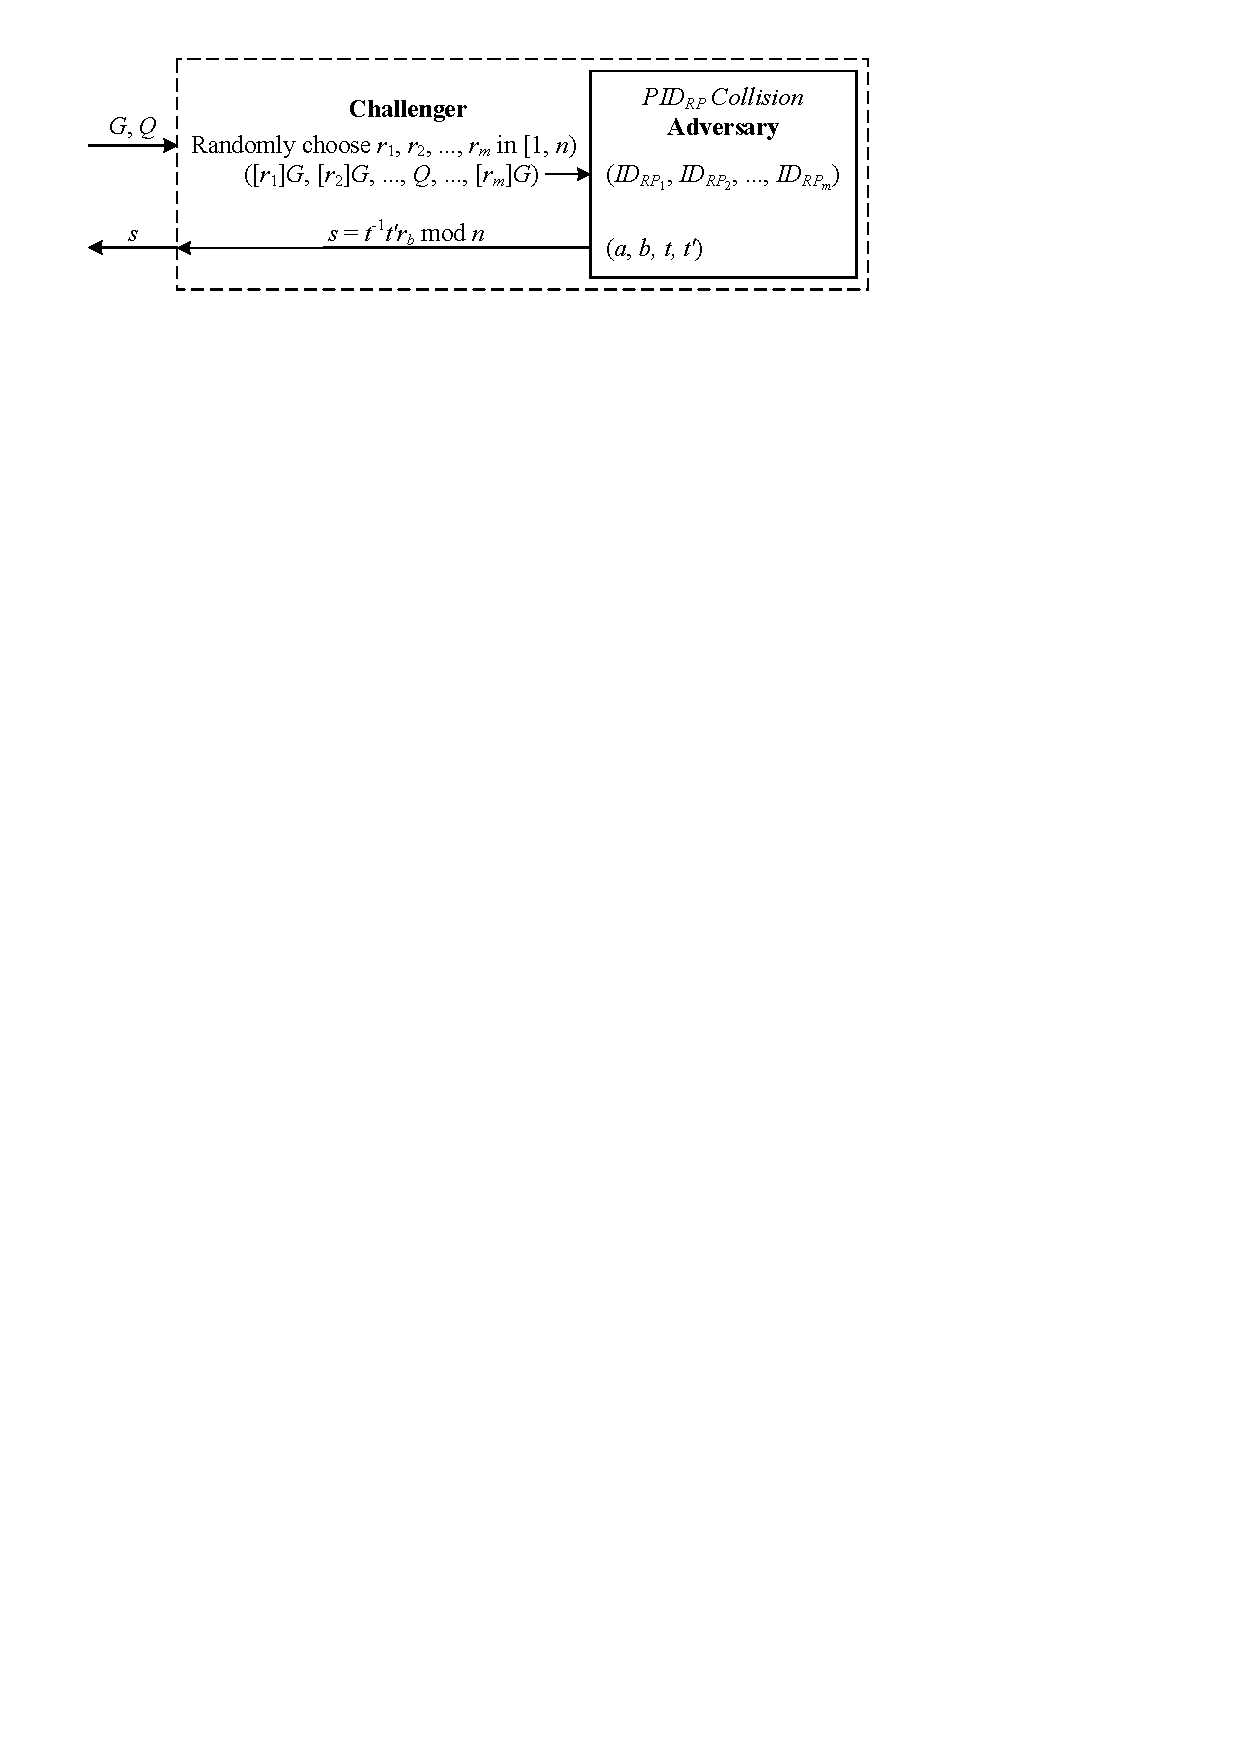
\includegraphics[width=0.96\linewidth]{fig/ecdlp_algorithm.pdf}
      \caption{The PPT algorithm $\mathcal{D}^*_c$ constructed based on the $PID_{RP}$ collision game to solve the ECDLP.}
      \label{fig:ecdlp_algorithm}
    \end{figure}
  
    The algorithm $\mathcal{D}^*_c$ works as below.
    The input of $\mathcal{D}^*_c$ is in the form of ($G, Q$). 
    On receiving an input ($G$, $Q$), 
    the challenger first randomly chooses $r_1, \cdots, r_m$ in $\mathbb{Z}_n$ to calculate $[r_1]G, \cdots, [r_m]G$.
    Then, it randomly chooses $j \in [1,m]$, replaces $[r_j]G$ with $Q$, and sends $m$ points to the adversary, 
    which returns the result ($a$, $b$, $t$, $t'$). 
    Finally, the challenger calculates $s = t^{-1}t'r_b \bmod n$ and returns $s$ as the output of $\mathcal{D}^*_c$.
  
    If the adversary succeeds in $\mathcal{G}_c$ and $[r_a]G$ happens to be replaced with $Q$, 
    then $\mathcal{D}^*_c$ outputs $s=t^{-1}t'r_b =x$ because $[tr_a]G = [t]Q = [t'r_b]G$. 
    For the adversary, $Q$ is indistinguishable from any other points in the input set, 
    as $[r_j]G$ is randomly replaced by the challenger.
    Hence, the probability of solving the ECDLP using $\mathcal{D}^*_c$ is formulated as:
    \begin{equation*}
      {\rm Pr}\{\mathcal{D}^*_c(G, [x]G)=x\} = {\rm Pr}\{s = x\}={\rm Pr}\{a=j\}{\rm Pr}_s=\frac{1}{m}{\rm Pr}_s
    \end{equation*}
  
    If the probability of finding $t$ and $t'$ satisfying $[tr]G = [t'r']G$ is non-negligible, 
    the adversary would also have non-negligible advantages in $\mathcal{G}_c$ and ${\rm Pr}_s$ regardless of the security parameter $\lambda$.
    Thus, we would find that ${\rm Pr}\{\mathcal{D}^*_c(G, [x]G)=x\}$ also becomes non-negligible even when $\lambda$ is sufficiently large, 
    because $m$ is a finite integer and $m \ll 2^\lambda$.
    This violates the ECDLP assumption. 
    Therefore, the probability of finding $t$ and $t'$ that satisfy $[tr]G = [t'r']G$ is negligible.
  \end{proof}
  
  Therefore, there is a contradication to the assumption, where we assumed that 
  $\myangle{n, Acct} \in d_{\emptyset}(S^j(\fAP{attacker}))$. 
  This shows every $\mathcal{U\!W\!S}^{auth}$ is secure in the sense of Property A.
  
  \subsection{Proof of Property B}
  As stated above, Property B is defined as follows:
  \begin{definition}\label{def:B}
    Let $\uppressoauthwebsystem$ be an \uppresso web system. We say that
    \emph{$\uppressoauthwebsystem$ is secure (with respect to Property B)} if
    for every run $\rho$ of $\uppressoauthwebsystem$, every state $(S^j, E^j, N^j)$
    in $\rho$, every $r\in \fAP{RP}$ that is honest in $S^j$, 
    every RP service token of the form $Acct$ recorded in
    $S^j(r).\str{serviceTokens}$, with the request corresponding to
    $\myangle{nonce, Acct}$ sent by some $b\in \fAP{B}$ which is honest in $S^j$, $b$ owns $Acct$.
  %Let $\mathcal{U\!W\!S}^{auth}$  be an UPPRESSO web system for authentication analysis. We say that $\mathcal{U\!W\!S}^{auth}$  is secure (with respect to Property A) if for every run $rho$ of $\mathcal{U\!W\!S}^{auth}$ , every state ($S^j$, $E^j$, $N^j$) in $rho$, every $r \in \mathtt{RP}$ that is honest in
  %$S^j$, every RP service token of the form $\langle IDToken$, $Acct \rangle$ recorded in $S^j$($r$).$\mathtt{serviceTokens}$, with the request corresponding to $\langle IDToken$, $Acct \rangle$ sent by some $b \in B$ which is honest in $S^j$, b owns Acct.
  \end{definition}
  
  First we call the request corresponding to $Acct$ (or service token request) $m$ and
  its response $m'$, and we refer to the state of $\uppressoauthwebsystem$ in the run 
  $\rho$ where $r$ processes $m$ by $s_l$. We are going to prove the $IDToken$ uploaded 
  by honest $b$ can only be related with the $Acct$ owned by $b$.
  
  %we follows the Lemma 10 and its proof in SPRESSO, which guarantees that the request corresponding to $\langle IDToken$, $Acct \rangle$ sent by honest $b$ is loaded from $script\_rp$. 
  %Then we are going to prove the $IDToken$ uploaded by honest $b$ can only be related with the $Acct$ owned by $b$ (which is quite different from SPRESSO).
  
  \begin{lemma}\label{lemma:request-m-is-from-script-rp}
    The request $m$ was sent by $\mi{script\_rp}$ loaded from 
    the origin $\an{d_r, \https}$ where $d_r$ is some domain of 
    $r$.
  \end{lemma}
  
  \begin{proof}
    The request $m$ is XSRF protected. In Algorithm~\ref{alg:rp}, 
    RP checks the presence of the Origin header and its value. 
    If the request $m$ was initiated by a document from a 
    different origin than $\an{d_r, \https}$, the honest browser 
    $b$ would have added an Origin header that would not 
    pass this test (or no Origin header at all), according to 
    the browser definition. The script $\mi{script\_rp}$ is the 
    only script that the honest party $r$ sends as a response 
    and that sends a request to $r$.
  \end{proof}
  
  \begin{lemma}
    For every $IDToken$ uploaded by honest $b$ during authentication, 
    the honest $r \in RP$ can always derive the service token of the form 
    $\myangle{n, \mi{Acct}}$ recorded in $S^j$($r$).$\mathtt{serviceTokens}$, where b owns Acct. 
  \end{lemma}
  \begin{proof}
    According to lemma~\ref{lemma:request-m-is-from-script-rp}, 
    we know that $m$ was sent by $\mi{script\_rp}$ loaded from an honest relying party. 
    The RP accepts the user's identity at line~\ref{line:add-service-token} in Algorithm~\ref{alg:rp}.
    And the user's identity at RP is generated at Line~\ref{line:gen-acct}, 
    based on the $PID_u$ retrieved from the IDToken and the trapdoor $t^{-1}$. 
    
    The $t^{-1}$ is generated and set at Line~\ref{line:gen-t}, 
    holding that $\mi{PID_{rp}}=[t]\mi{ID_{rp}}$.
    Originally, $t$ is chosen by $\mi{script\_idp}$ at Line~\ref{line:gen-t}, Algorithm~\ref{alg:uppresso-script-idp} 
    and transmit to RP through $\mi{script\_rp}$.
    \newc
    Similar to lemma~\ref{lemma:script-idp-to-script-rp} and lemma~\ref{lemma:script-rp-to-rp}, 
    we can prove that RP can only receive the $t$ from $\mi{script\_idp}$, so the $t$ in both parties is equal.
    \oldc

    The $\mi{script\_idp}$ also receives a cert signed by the IdP from the honest RP and verify the cert at Line~\ref{alg:script-idp-verify-cert}, Algorithm~\ref{alg:uppresso-script-rp}.
    After that, $\mi{script\_idp}$ calculates $\mi{PID_{rp}}$ using $t$ and $\mi{ID_{rp}}$ from the cert.
    \newc
    Since $t$ in both parties is equal and $\mi{ID_{rp}}$ is guaranteed by the cert's signature, 
    we can have that the $\mi{PID_{rp}}$ in $\mi{script\_idp}$ and RP is equal.
    \oldc

    Then $\mi{script\_idp}$ sends a request to IdP bringing $\mi{PID_{rp}}$ for the IDToken 
    at Line~\ref{line:send-pidrp} in Algorithm~\ref{alg:uppresso-script-idp}.
    IdP adds the $\mi{PID_{rp}}$ from $\mi{script\_idp}$ into the IDToken.
    \newc
    Therefore, we can see that 
    $\mi{IDToken}.\mi{PID_{rp}}=[t]\mi{ID_{rp}}$ meaning that it is the same as in RP.
    \oldc

    The IDToken is issued at Line~\ref{line:sign-token} in Algorithm~\ref{alg:idp}.
    The IdP generates the $PID_u$ based on the $PID_{rp}$ and $ID_u$.
    \newc
    According to lemma~\ref{lemma:b-trigger-request}, 
    the identities IdP accept and store is from the honest browser, 
    and the honest browser can only provide its own usernames and passwords 
    because only $\mi{script\_idp}$ or its child window has the access to these credentials 
    according to lemma~\ref{lemma:script-idp-trigger-request}.
    Therefore, attacker cannot alter the username and password sent to IdP.
    Since the username and password are owned by the honest browser and 
    $ID_u$ is mapped to this credential at Line~\ref{line:get-idu} in Algorithm~\ref{alg:idp}. 
    Now we can see that the $ID_u$ used to generate IDToken must be owned by the browser 
    and $\mi{IDToken}.\mi{PID_{u}}=[\mi{ID_u}]\mi{PID_{rp}}$.
    

    %In summary, for every IDToken sent by honest $b$ and IdP, there must be 
    %$\mi{IDToken}.\mi{PID_{rp}} \equiv [t]\mi{ID_{rp}} \equiv \mi{PID_{rp}}$ and 
    %$\mi{IDToken}.\mi{PID_{u}} \equiv [\mi{ID_u}]\mi{PID_{rp}}$. 
    %According to lemma~\ref{user-identification}, 
    Therefore, the $Acct$ calculated by RP following Equation~\ref{equ:calc-acct} must uniquely identifies the user $ID_u$ which is owned by honest $b$.  
    \oldc
    \begin{equation}\label{equ:calc-acct}
      \begin{split}
      Acct=[t^{-1}]PID_u=[t^{-1}][ID_u]PID_{rp}=\\
      [t^{-1}utr]G =[ur]G=[ID_U]ID_{RP}
      \end{split}
    \end{equation}
  \end{proof}

%对于给定的任意一个ID_{RP},for each ID_U in Z_n,都有Acct = [id_u]ID_RP是unique。
 
  With the above proofs, we now can guarantee that every 
  $\uppressoauthwebsystem$ system satisfies the requirements in 
  Definition~\ref{def:B}, therefore $\uppressoauthwebsystem$ 
  must be secure of Property B.
  
  These prove Theorem~\ref{thm:authentication}.\QED
  
  \section{Proof of Privacy against IdP-based Login Tracing}
  
  In our privacy analysis, we show that an identity provider in UPPRESSO cannot learn 
  where its users log in. We formalize this property as an indistinguishability 
  property: an identity provider (modeled as a web attacker) cannot distinguish 
  between a user logging in at one relying party and the same user logging in at 
  a different relying party.
  
  We will here first describe the precise model that we use for privacy.
  After that, we define an equivalence relation between configurations,
  which we will then use in the proof of privacy.
  
  \subsection{Formal Model of UPPRESSO for Privacy Analysis}
  
  \begin{definition}[Challenge Browser]
    Let $\mi{dr}$ some domain and $b(\mi{dr})$ a DY process. 
    We call $b(\mi{dr})$ a \emph{challenge browser} iff $b$
    is defined exactly the same as a browser with two exceptions: 
    (1) the state contains one more property, namely 
    $\mi{challenge}$, which initially contains the term $\top$. 
    (2) The broswer's algorithm is extended by the following at 
    its very beginning: It is checked if a message $m$ is 
    addressed to the domain $\str{CHALLENGE}$ (which we call the 
    challenger domain). If $m$ is addressed to this domain and 
    no other message $m'$ was addressed to this domain before 
    (i.e., $\mi{challenge} \not\equiv \bot$), then $m$ is changed 
    to be addressed to the domain $\mi{dr}$ and $\mi{challenge}$ 
    is set to $\bot$ to recorded that a message was addressed to 
    $\str{CHALLENGE}$.
  \end{definition}
  
  \begin{definition}[Deterministic DY Process]
    We call a DY process $p = (I^p,Z^p,R^p,s_0^p)$ \emph{deterministic} iff 
    the relation $R^p$ is a (partial) function.
  
    We call a script $R_\text{script}$ \emph{deterministic} iff the relation 
    $R_\text{script}$ is a (partial) function.
  \end{definition}

  \newc
  \begin{definition}[Distinguished Attacker]
    If $(\websystem, \scriptset,\mathsf{script}, E^0)$ is
    a web system and $p$ is an attacker process in
    $\websystem$, then we say that $(\websystem,
    \scriptset,\mathsf{script}, E^0,p)$ is a \emph{web
    system with a distinguished attacker process $p$}. 
  \end{definition}
  \oldc

  The disitinguished attacker process is a web attacker and 
  can receive all the data from other attacker processes, 
  so when we talk about indistinguishability of a system, 
  we will only analyze the state of the disitinguished attacker process.
  
  \begin{definition}[\uppresso Web System for Privacy Analysis]\label{def:uppresso-ws-priv}
    Let $\uppressowebsystem = (\bidsystem, \scriptset, 
    \mathsf{script}, E^0)$ be an UPPRESSO web system with 
    $\bidsystem = \mathsf{Hon} \cup \mathsf{Web} \cup \mathsf{Net}$, 
    $\mathsf{Hon} = \fAP{B} \cup \fAP{RP} \cup \fAP{IDP}$.
    (as described in Appendix~\ref{app:outlineuppressomodel}).
    $\fAP{RP} = \{r_1,r_2\}$, $r_1$ and $r_2$ two (honest) relying parties,
    Let $\fAP{attacker} \in \mathsf{Web}$ be some web attacker and also a distinguished attacker.
    Let $\mi{dr}$ be a domain of $r_1$ or $r_2$ and $b(\mi{dr})$ a challenge browser. 
    Let $\mathsf{Hon}' := \{ b(\mi{dr}) \} \cup \fAP{RP}$, 
    $\mathsf{Web}' := \mathsf{Web}$, 
    and $\mathsf{Net}' := \emptyset$ (i.e., there is no network attacker).
    Let $\bidsystem' := \mathsf{Hon}' \cup \mathsf{Web}' \cup \mathsf{Net}'$.  
    Let $\scriptset' := \scriptset$ and $\mathsf{script}'$ be accordingly.
    We call $\uppressoprivwebsystem(\mi{dr}) = (\bidsystem', \scriptset', \mathsf{script}', E^0, \fAP{attacker})$ 
    an \emph{\uppresso web system for privacy analysis} 
    iff the domain $\mi{dr}_1$ the only domain assigned to $r_1$, and
    $\mi{dr}_2$ the only domain assigned to $r_2$. The browser
    $b(\mi{dr})$ owns exactly one identity and this identity
    is governed by some attacker.  All honest parties (in
    $\mathsf{Hon}$) are not corruptible, i.e., they ignore any
    $\str{CORRUPT}$ message. Identity providers are assumed to be
    dishonest, and hence, are subsumed by the web attackers (which
    govern all identities). %In the initial state $s_0^b$ of the (only)
    %browser in $\bidsystem'$ and in the initial states $s_0^{r_1}$,
    %$s_0^{r_2}$ of both relying parties, the DNS address is
    %$\mapAddresstoAP(\fAP{dns})$. Further, $\mi{wkCache}$ in the initial
    %states $s_0^{r_1}$, $s_0^{r_2}$ is equal and contains a public key
    %for each domain registered in the DNS server (i.e., 
    the relying
    parties already know some public key to verify \uppresso identity
    assertions from all domains known in the system and they do not have to fetch them from IdP.
  \end{definition}
  
  As all parties in an \uppresso web system for privacy analysis are either web 
  attackers, browsers, or deterministic processes and all scripting processes are 
  either the attacker script or deterministic, it is easy to see that in \uppresso 
  web systems for privacy analysis with configuration $(S,E,N)$ a command $\zeta$ 
  induces at most one processing step. We further note that, under a given infinite 
  sequence of nonces $N^0$, all schedules $\sigma$ induce at most one run 
  $\rho = ((S^0,E^0,N^0),\dots,(S^i,E^i,N^i),\dots,(S^{|\sigma|},E^{|\sigma|},N^{|\sigma|}))$ 
  as all of its commands induce at most one processing step for the $i$-th configuration.
  
  We will now define our privacy property for \uppresso:
  
  \begin{definition}[IdP-Privacy]\label{def:idp-privacy}
    Let 
    \begin{align*}
      \uppressoprivwebsystem_1 := \uppressoprivwebsystem(\mi{dr}_1) =
      (\bidsystem_1, \scriptset, \mathsf{script}, E^0, \fAP{attacker}_1)&\text{ and}\\
      \uppressoprivwebsystem_2 := \uppressoprivwebsystem(\mi{dr}_2) =
      (\bidsystem_2, \scriptset, \mathsf{script}, E^0, \fAP{attacker}_2)&
    \end{align*}
    be \uppresso web systems for privacy analysis.  Further, we require
    $\fAP{attacker}_1 = \fAP{attacker}_2 =: \fAP{attacker}$ and for $b_1
    := b(\mi{dr}_1)$, $b_2 := b(\mi{dr}_2)$ we require $S(b_1) = S(b_2)$
    and $\bidsystem_1 \setminus \{b_1\} = \bidsystem_2 \setminus
    \{b_2\}$ (i.e., the web systems are the same up to the parameter of
    the challenge browsers).  We say that $\uppressoprivwebsystem$ is
    \emph{IdP-private} iff $\uppressoprivwebsystem_1$ and
    $\uppressoprivwebsystem_2$ are indistinguishable.
  \end{definition}
  
  \subsection{Definition of Equivalent Configurations}\label{app:defin-equiv-stat}
  
  Let $\uppressoprivwebsystem_1 = (\bidsystem_1, \scriptset, \mathsf{script}, E^0, \fAP{attacker})$ 
  and $\uppressoprivwebsystem_2 = (\bidsystem_2, \scriptset, \mathsf{script}, E^0, \fAP{attacker})$ 
  be \uppresso web systems for privacy analysis. Let $(S_1,E_1,N_1)$ 
  be a configuration of $\uppressoprivwebsystem_1$ and $(S_2,E_2,N_2)$ 
  be a configuration of $\uppressoprivwebsystem_2$.
  
  \begin{definition}[Proto-Tags]
    We call a term of the form $[t]R$ with the variable
    $R$ as a placeholder for an $ID_{rp}$, and $t$ some nonces a
    \emph{proto-tag}.
  \end{definition}
  
  \begin{definition}[Term Equivalence up to Proto-Tags]
    Let $\theta = \{a_1, \ldots, a_l \}$ be a finite set of proto-tags.
    Let $t_1$ and $t_2$ be terms. We call $t_1$ and $t_2$
    \emph{term-equivalent under a set of proto-tags $\theta$} iff there
    exists a term $\tau \in \terms(\{x_1,\dots,x_l\})$ such that
    $t_1 = (\tau [ a_1 / x_1 , \dots , a_l / x_l ])[ ID_{\mi{dr}_1} / R ]$ and
    $t_2 = (\tau [ a_1 / x_1 , \dots , a_l / x_l ])[ ID_{\mi{dr}_2} / R ]$.
    We write $t_1 \prototagequiv{\theta} t_2$.
  
    We say that two finite sets of terms $D$ and $D'$ are
    \emph{term-equivalent under a set of proto-tags $\theta$} iff
    $|D| = |D'|$ and, given a lexicographic ordering of the elements in
    $D$ of the form $(d_1,\dots,d_{|D|})$ and the elements in $D'$ of
    the form $(d'_1,\dots,d_{|D'|})$, we have that for all
    $i \in \{1,\dots,|D|\}$: $d_i \prototagequiv{\theta} d'_i$. We then
    write $D \prototagequiv{\theta} D'$.
  \end{definition}
  
  %随机数t的情况
  \begin{definition}[Equivalence of HTTP Requests]
    Let $m_1$ and $m_2$ be (potentially encrypted) HTTP requests, 
    $L$ be a set of login session tokens and
    $\theta = \{a_1, \ldots, a_l \}$ be a finite set of proto-tags. 
    We call $m_1$ and $m_2$ \emph{$\delta$-equivalent under a set of proto-tags $\theta$} 
    iff $m_1 \prototagequiv{\theta} m_2$ or all subterms are equal with the following exceptions:
    \begin{enumerate}
    \item the Host value and the Origin/Referer headers in both requests
      are the same except that the domain $\mi{dr}_1$ in $m_1$ can be
      replaced by $\mi{dr}_2$ in $m_2$,
    \item If the cookie in both requests include $\str{loginSessionToken}$, 
      then there exists an $l' \in L$ such that $g_1[\str{loginSessionToken}] \equiv l'$, and
    \item the HTTP body $g_1$ of $m_1$ and the HTTP body $g_2$ of $m_2$
      are (I) term-equivalent under $\theta$, 
      (II) for $j\in \{1,2\}$ if
      $g_j[\str{IDToken}] \sim \myangle{PID_{dr_j}, [*]PID_{dr_j}, 
      \sig{\myangle{PID_{dr_j}, [*]PID_{dr_j}}}{*}}$
      and the origin (HTTP header) of HTTP message in $m_j$ is
      $\an{\mi{dr}_j,\https}$ then the receiver of this message is
      $r_j$, and 
    \item if $m_1$ is an encrypted HTTP request then and only then $m_2$
      is an encrypted HTTP request and the keys used to encrypt the
      requests have to be the correct keys for $\mi{dr}_1$ and
      $\mi{dr}_2$ respectively.
    \end{enumerate}
    We write $m_1 \httptagequiv{\theta} m_2$.
  \end{definition}
  
  %loginsessionrecord := <t, tag>
  \begin{definition}[Extracting Entries from Login Sessions]
    Let $t_1$, $t_2$ be dictionaries over $\nonces$ and $\terms$,
    $\theta$ be a finite set of proto-tags, and $d$ a domain. We call
    $t_1$ and $t_2$ \emph{$\eta$-equivalent} iff $t_2$ can be
    constructed from $t_1$ as follows: For every proto-tag
    $a \in \theta$, we remove the entry identified by the dictionary key
    $i$ for which it holds that $\proj{2}{t_1[i]} \equiv a[ID_r/ R]$, if
    any. We denote the set of removed entries by $D$. We write
    $\logsessminus{t_1}{t_2}{\theta}{r}{D}$.
  \end{definition}
  
  \begin{definition}
    Let $a$ be a proto-tag, $S_1$ and $S_2$ be states of \uppresso web
    systems for privacy analysis, and $l$ a nonce. We call $l$ a login
    session token for the proto-tag $a$, written
    $l \in \mathsf{loginSessionTokens}(a,S_1,S_2)$ iff for any
    $i \in \{1,2\}$ and any $j \in \{1,2\}$ we have that
    $\proj{2}{S_i(r_j).\str{loginSessions}[l]} = a[ID_{dr_j}/ R]$.
  \end{definition}
  
  \begin{definition}[Equivalence of States]\label{def:eq-of-states}
    Let $\theta$ be a set of proto-tags and 
    %$H$ be a set of nonces. 
    $L$ be a set of login session tokens.
    Let $T:=\{t\mid [t]R\in \theta\}$. 
    We call $S_1$ and $S_2$ \emph{$\gamma$-equivalent under 
    $(\theta, L)$} iff the following conditions are met:
    \begin{enumerate}
    \item\label{eqs:r1} $S_1(\fAP{r_1})$ equals $S_2(\fAP{r_1})$ except
      for the subterms $\str{loginSessions}$ and $\str{serviceTokens}$, and
    \item\label{eqs:r2} $S_1(\fAP{r_2})$ equals $S_2(\fAP{r_2})$ except
      for the subterms $\str{loginSessions}$ and $\str{serviceTokens}$, and
    \item\label{eqs:logsess} for two sets of terms $D$ and $D'$:
      $\logsessminus{S_1(\fAP{r_1}).\str{loginSessions}}{S_2(\fAP{r_1}).\str{loginSessions}}{\theta}{\mi{dr}_1}{D}$,
      $\logsessminus{S_2(\fAP{r_2}).\str{loginSessions}}{S_1(\fAP{r_2}).\str{loginSessions}}{\theta}{\mi{dr}_2}{D'}$,
      and $D \prototagequiv{\theta} D'$, and
    \item\label{eqs:att-not-t} $\forall t \in T$:
      $t \not\in d_\emptyset(\bigcup_{i \in \{1,2\},\ A\, \in\, \mathsf{Web}\, \cup \,
      \mathsf{Net}\, 
      %\cup\, \{\mathsf{dns}, \mathsf{fwd}
      \}}S_i(A))$
    \item\label{eqs:att} for each attacker $A$:
      $S_1(A) \prototagequiv{\theta} S_2(A)$, and
    \item\label{eqs:att-not-l} for all $a\in\theta$ and all attackers $A$ we have that
      $\nexists\ l \in \mathsf{loginSessionTokens}(a,S_1,S_2)$ such that
      $l$ is a subterm of $S_1(A)$ or $S_2(A)$.
    \item\label{eqs:b} $S_1(b_1)$ equals $S_2(b_2)$ except for for the
      subterms $\str{challenge}$, $\str{windows}$
      %, $\str{pendingDNS}$, $\str{pendingRequests}$ 
      and we have that
      \begin{enumerate}
      \item \label{eqs:b:challenge}
        $S_1(b_1).\str{challenge} = \mi{dr}_1 \wedge
        S_2(b_2).\str{challenge} = \mi{dr}_2$
        or $S_1(b_1).\str{challenge} = S_2(b_2).\str{challenge} = \bot$,
        and
      \item $S_1(b_1).\str{windows}$ equals $S_2(b_2).\str{windows}$ with
        the exception of the subterms $\str{location}$, $\str{referrer}$,
        $\str{scriptstate}$, and $\str{scriptinputs}$ of some document terms
        pointed to by $\mathsf{Docs}^+(S_1(b_1)) = \mathsf{Docs}^+(S_2(b_2)) =: J$. 
        For all $j \in J$ we have that: \label{eqs:b:w}
        \begin{enumerate}
        \item there is no $t \in T$ such that
          \begin{align*}
            t \in d_{\nonces \setminus \{t\}}(\{&S_1(b_1).j.\str{location}
            ,  S_2(b_2).j.\str{location},\\ & S_1(b_1).j.\str{referrer} , 
            S_2(b_2).j.\str{referrer}\})
          \end{align*}
        \item for $p \in \{$
          \begin{align*}
            & \an{\tXMLHTTPRequest,*,*},\\
            & \an{\tPostMessage,*,\an{\mapDomain(dr_j), \https},\an{\str{t}, *}},\\
            & \an{\tPostMessage,*,\an{\mapDomain(dr_j), \https},\an{\str{IDToken}, *}}\\
            & \an{\tPostMessage,*,\an{\mapDomain(idp), \https},\an{\str{Cert}, *}}
          \end{align*}
          $\}$ we have
          $S_1(b_1).j.\str{scriptinputs} |\, p \prototagequiv{\theta}
          S_2(b_2).j.\str{scriptinputs} |\, p$, and
        \item\label{eqs:b:w:script_rp} if
          $S_1(b_1).j.\str{origin} \in \{\an{\mi{dr}_1, \https},\an{\mi{dr}_2, \https}\}$
          then $S_1(b_1).j.\str{script} \equiv \str{script\_rp}$ and \
          \begin{enumerate}
          \item $S_1(b_1).j.\str{location}$ and $S_2(b_2).j.\str{location}$
            are term-equivalent under $\theta$ except for the host part,
            which is either equal or $\mi{dr}_1$ in $b_1$ and $\mi{dr}_2$ in
            $b_2$, and
          \item $S_1(b_1).j.\str{referrer}$ and $S_2(b_2).j.\str{referrer}$
            are term-equivalent under $\theta$ except for the host part,
            which is either equal or $\mi{dr}_1$ in $b_1$ and $\mi{dr}_2$ in
            $b_2$, and
          \item
            $S_1(b_1).j.\str{scriptstate} \prototagequiv{\theta}
            S_2(b_2).j.\str{scriptstate}$ and if $\exists\, l \in L$ such that $l$ is a subterm of $S_1(b_1).j.\str{scriptstate}$, then $S_1(b_1).j.\str{location}.\str{host} \equiv \mi{dr}_1$ and $S_2(b_2).j.\str{location}.\str{host} \equiv \mi{dr}_2$, and
          \item if $\exists\, l \in L$ such that $l$ is a subterm of
            $S_1(b_1).j.\str{scriptinputs}$, then
            $S_1(b_1).j.\str{location}.\str{host} \equiv \mi{dr}_1$ and
            $S_2(b_2).j.\str{location}.\str{host} \equiv \mi{dr}_2$, and
          %\item $\forall t \in N$: $t$ is not contained in any subterm of
          %  $S_1(b_1).j.\str{scriptstate}$ except for
          %  $S_1(b_1).j.\str{scriptstate}.\str{parameters}$, and
          %  \begin{itemize}
          %  \item
          %    $S_1(b_1).j.\str{origin} \not\equiv
          %    \an{\mi{dr}_1,\https}$\\$\implies
          %    t \not\equiv S_1(b_1).j.\str{scriptstate}.\str{parameters}$, and
          %  \item $S_1(b_1).j.\str{origin}
          %    \not\equiv
          %    \an{\mi{dr}_1,\https}$\\$\implies t \not\in
          %    d_\emptyset(S_1(b_1).j.\str{scriptinputs})$, and
          %  \item
          %    $S_2(b_2).j.\str{origin} \not\equiv
          %    \an{\mi{dr}_2,\https}$\\$\implies
          %    t \not\equiv S_2(b_2).j.\str{scriptstate}.\str{parameters}$, and
          %  \item $S_2(b_2).j.\str{origin}
          %    \not\equiv
          %    \an{\mi{dr}_2,\https}$\\$\implies t \not\in
          %    d_\emptyset(S_2(b_2).j.\str{scriptinputs})$,
          %    and \end{itemize}
          \end{enumerate}
        \item\label{eqs:b:w:att_script} if
          $S_1(b_1).j.\str{origin} \not\in
          \{\an{\mi{dr}_1,\https},\an{\mi{dr}_2,\https}\}$
          then $S_1(b_1).j.\str{script} \equiv \str{script\_idp}$ and \
          \begin{enumerate}
          \item
            $S_1(b_1).j.\str{location} \prototagequiv{\theta}
            S_2(b_2).j.\str{location}$, and
          \item
            $S_1(b_1).j.\str{referrer} \prototagequiv{\theta}
            S_2(b_2).j.\str{referrer}$, and
          \item\label{eqs:b:w:att_script:state}
            $S_1(b_1).j.\str{scriptstate} \prototagequiv{\theta}
            S_2(b_2).j.\str{scriptstate}$, and
          \item
            $S_1(b_1).j.\str{scriptinputs} \prototagequiv{\theta}
            S_2(b_2).j.\str{scriptinputs}$, and
          \item\label{eqs:b:w:att_script:t}
            $\forall t \in T$: $t$ is not contained in any subterm of 
            $S_1(b_1).j.\str{scriptstate}$ except for 
            $S_1(b_1).j.\str{scriptstate}.\mi{parameters}[\str{t}]$, and
          \item $\nexists\, l \in L$ such that $l$ is a subterm of
            $S_1(b_1).j.\str{scriptstate}$ or of
            $S_1(b_1).j.\str{scriptinputs}$, and
          \end{enumerate}
        \end{enumerate}
      \item\label{eqs:b:misc} for
        $x \in \{\str{cookies},\str{localStorage},\str{sessionStorage},\str{sts}\}$
        we have that $S_1(b_1).x \prototagequiv{\theta} S_2(b_2).x$. For the
        domains $\mi{dr}_1$ and $\mi{dr}_2$ there are no entries in the
        subterms $x$.
      \end{enumerate}
    \end{enumerate}
  \end{definition}
  
  \begin{definition}[Equivalence of Events]\label{def:Events}
    Let $\theta$ be a set of proto-tags, 
    $L$ be a set of login session tokens, 
    $H$ be a set of nonces, and
    $T:=\{t\mid [t]R\in \theta\}$. 
    We call $E_1 = (e_1^{(1)}, e_2^{(1)}\dots)$ and
    $E_2= (e_1^{(2)}, e_2^{(2)} \dots)$ 
    \emph{$\beta$-equivalent under $(\theta, L, H)$} 
    iff all of the following conditions are satisfied for every 
    $i \in \mathbb{N}$:
  
    \begin{enumerate}
      \item\label{eqe:distinction} One of the following conditions holds
        true:
        \begin{enumerate}
        \item\label{eqe:prototagequiv}
          $e_i^{(1)} \prototagequiv{\theta} e_i^{(2)}$ and if $e_i^{(1)}$
          contains an HTTP(S) message (i.e., HTTP(S) request or HTTP(S)
          response), then the HTTP nonce of this HTTP(S) message is not
          contained in $H$, or
        \item\label{eqe:http-req} $e_i^{(1)}$ is an HTTP request $m_1$
          from $b_1$ to $r_1$ and $e_i^{(2)}$ is an HTTP request $m_2$
          from $b_2$ to $r_2$, $m_1 \httptagequiv{\theta} m_2$, and both
          requests are unencrypted or encrypted (i.e., $m_1$ and $m_2$ are
          the content of the encryption) and $m_1.\str{nonce} \in H$, or
        \item\label{eqe:http-res} $e_i^{(1)}$ is an HTTP(S) response from
          $r_1$ to $b_1$ and $e_i^{(2)}$ is an HTTP(S) response from $r_2$
          to $b_2$, and their HTTP messages $m_1$ (contained in
          $e_i^{(1)}$) and $m_2$ (contained in $e_i^{(1)}$) are the same
          except for the HTTP body $g_1 := m_1.\str{body}$ and the HTTP
          body $g_2 := m_2.\str{body}$ which have to be
          $g_1 \prototagequiv{\theta} g_2$ and $m_1.\str{nonce} \in H$.
        \end{enumerate}
      %可能破坏PID_rp不可区分性的参数需要单独列出
      \item\label{eqe:pre:l} If there exists $l \in L$ such that $l$ is a
        subterm of $e_i^{(1)}$ or $e_i^{(2)}$ then we have that
        $e_i^{(1)}$ is a message from $b_1$ to $r_1$ and $e_i^{(2)}$ is a
        message from $b_2$ to $r_2$ or we have that $e_i^{(1)}$ is a
        message from $r_1$ to $b_1$ and $e_i^{(2)}$ is a message from
        $r_2$ to $b_2$.
      \item\label{eqe:pre:t} If there exists $t \in T$ such that
        $t \in d_{\nonces\setminus\{t\}}(\{e_i^{(1)}, e_i^{(2)}\})$ 
        then $e_i^{(1)}$ is an HTTP(S) request from $b_1$ to $r_1$ 
        and $e_i^{q(2)}$ is an HTTP(S) request from $b_2$ to $r_2$ 
        and the bodies of both HTTP messages are of the form
        $\an{\an{\str{t}, t}}$.
      \item\label{eqe:pre:rp-scripts} If $e_i^{(1)}$ or $e_i^{(2)}$ is an
        HTTP(S) response with body $g$ from a relying party, then it does
        not contain any $\str{Location}$ or $\cSTS$ header
        and if $\proj{1}{g}$ is a string representing a script, then
        $\proj{1}{g}$ is $\str{script\_rp}$.
      \item\label{eqe:pre:unencrypted-http} If $e_i^{(1)}$ or $e_i^{(2)}$
        is an unencrypted HTTP response, then the message was sent by some
        attacker.
    \end{enumerate}
  \end{definition}
  
  \begin{definition}[Equivalence of Configurations]
    We call $(S_1,E_1,N_1)$ and $(S_2,E_2,N_2)$
    \emph{$\alpha$-equivalent} iff there exists a set of proto-tags
    $\theta$ and a set of nonces $H$ such that $S_1$ and $S_2$ are
    $\gamma$-equivalent under $(\theta,H)$, $E_1$ and $E_2$ are
    $\beta$-equivalent under $(\theta,L,H)$ for
    $L := \bigcup_{a\in\theta} \mathsf{loginSessionTokens}(a,S_1,S_2)$,
    and $N_1 = N_2$.
  \end{definition}
  
  \subsection{Privacy Proof}
  
  \begin{theorem} \label{theorem:A}Every UPPRESSO web system for privacy analysis is IdP-private.
  \end{theorem}
  
  Let $\mathcal{U\!W\!S}^{priv}$ be UPPRESSO web system for privacy analysis.\par
  To prove Theorem \ref{theorem:A}, we have to show that the UPPRESSO web systems $\mathcal{U\!W\!S}^{priv}_1$ and $\mathcal{U\!W\!S}^{priv}_2$ 
  are indistinguishable. To show the indistinguishability of $\mathcal{U\!W\!S}^{priv}_1$ and $\mathcal{U\!W\!S}^{priv}_2$, 
  we show that they are indistinguishable under all schedules $\sigma$.
  For this , we first note that for all $\sigma$, there is only one run induced by each $\sigma$(as our web system, when scheduled, is deterministic).
  We now proceed to show that for all schedules $\sigma=(\zeta _1, \zeta_2,\dots)$, iff $\sigma$ induces a run $\sigma(\mathcal{U\!W\!S}^{priv}_1)$ there exists a run $\sigma(\mathcal{U\!W\!S}^{priv}_2)$ such that $\sigma(\mathcal{U\!W\!S}^{priv}_1)\approx\sigma(\mathcal{U\!W\!S}^{priv}_1)$\par
  We now show that if two configurations are $\alpha$-equivalent, then the view of the attacker is statically equivalent.
  
  \begin{lemma}
    Let $(S_1,E_1,N_1)$ and $(S_2,E_2,N_2)$ be two 
    $\alpha$-equivalent configurations. 
    Then $S_1(attacker)\approx S_2(attacker)$.
  \end{lemma}
  \begin{proof}
    From the $\alpha$-equivalence of $(S_1,E_1,N_1)$ and 
    $(S_2,E_2,N_2)$ it follows that $S_1(\fAP{attacker}) 
    \prototagequiv{\theta} S_2(\fAP{attacker})$.
    From Condition~\ref{eqs:att-not-t} for $\gamma$-equivalence 
    it follows that
    $t \not\in d_\emptyset(\bigcup_{i \in \{1,2\},\ A\, \in\, 
    \mathsf{Web}\, \cup \, \mathsf{Net}\, \}}S_i(A))$
    (i.e., the attacker does not know any keys for the tags 
    contained in its view), and with Lemma~\ref{thm-idp-untraceability-new} it is easy to see 
    that the views are statically equivalent.
  \end{proof}

  \newc
  \begin{lemma}\label{thm-idp-untraceability-new}
    Given a point on the elliptic curve denoted by $[r]G$, 
    an adversary cannot distinguish $[tr]G$ from a random variable on $\mathbb{E}$, 
    where $t$ is random in $\mathbb{Z}_n$ and unknown to the adversary.
  \end{lemma}
  \begin{proof}
    Consider a finite cyclic group $\mathbb{E}$ where the number of points on $\mathbb{E}$ is $n$. 
    Because $G$ is a generator of order $n$, $[r]G$ is also a generator on $\mathbb{E}$ of order $n$. 
    $t$ is randomly chosen in $\mathbb{Z}_n$ and always kept unknown to the adversary. 
    Therefore, $[tr]G$ is \emph{indistinguishable} from a point $Q$ that is randomly chosen on $\mathbb{E}$.\cite{oprf-proved,voprf-proved}.
  \end{proof}
  \oldc
  
  We now show that $\sigma(\uppressoprivwebsystem_1) \approx
  \sigma(\uppressoprivwebsystem_2)$ by induction over the length 
  of $\sigma$. We first, in Lemma~\ref{lemma:initial-config-private}, 
  show that $\alpha$-equivalence (and therefore, indistinguishability 
  of the views of $\fAP{attacker}$) holds for the initial 
  configurations of $\uppressoprivwebsystem_1$ and 
  $\uppressoprivwebsystem_2$. We then, in 
  Lemma~\ref{lemma:step-config-private}, show that for each 
  configuration induced by a processing step in $\zeta$,
  $\alpha$-equivalence still holds true.
  
  \begin{lemma}\label{lemma:initial-config-private}
    The initial configurations $(S_1^0,E^0,N^0)$ of 
    $\mathcal{U\!W\!S}^{priv}_1$ and $(S_2^0,E^0,N^0)$ of 
    $\mathcal{U\!W\!S}^{priv}_2$ are $\alpha$-equivalent.
  \end{lemma}
  \begin{proof}
    We now have to show that there exists a set of proto-tags $\theta$ and a set of nonces $H$
    such that $S_1^0$ and $S_2^0$ are $\gamma$-equivalent under
    $(\theta,H)$, $E_1^0 = E^0$ and $E_2^0 = E^0$ are $\beta$-equivalent
    under $(\theta,L,H)$ with $L := \bigcup_{a\in\theta} \mathsf{loginSessionTokens}(a,S_1,S_2)$, and $N_1^0 = N_2^0 = N^0$.
  
    Let $\theta = H = L = \emptyset$. Obviously, both latter conditions are
    true. For all parties $p \in \bidsystem_1 \setminus \{b_1\}$, it is
    clear that $S_1^0(p) = S_2^0(p)$. Also the states $S_1^0(b_1)$ and
    $S_2^0(b_2)$ are equal. Therefore, all conditions
    of Definition~\ref{def:eq-of-states} are fulfilled. Hence, the
    initial configurations are $\alpha$-equivalent.
  \end{proof}
  
  \begin{lemma}\label{lemma:step-config-private}
    Let $(S_1,E_1,N_1)$ and $(S_2,E_2,N_2)$ be two 
    $\alpha$-equivalent configurations of 
    $\uppressoprivwebsystem_1$ and $\uppressoprivwebsystem_2$, 
    respectively. Let $\zeta = \an{\mi{ci},\mi{cp}, 
    \tau_\text{process}, \mi{cmd}_\text{switch}, 
    \mi{cmd}_\text{window},\tau_\text{script},\mi{url}}$
    be a web system command. Then, $\zeta$ induces a processing 
    step in either both configurations or in none. In the latter 
    case, let $(S_1',E_1',N_1')$ and $(S_2',E_2',N_2')$ be 
    configurations induced by $\zeta$ such that
    \[(S_1,E_1,N_1) \xrightarrow{\zeta} (S_1',E_1',N_1') \quad 
    \text{and} \quad (S_2,E_2,N_2) \xrightarrow{\zeta} 
    (S_2',E_2',N_2') \ .\]
    Then, $(S_1',E_1',N_1')$ and $(S_2',E_2',N_2')$ are
    $\alpha$-equivalent.  
  \end{lemma}
  \begin{proof}
    Let $\theta$ be a set of proto-tags and $H$ be a set of 
    nonces for which $\alpha$-equivalence holds and let 
    $L:=\bigcup_{a\in\theta}\text{loginSessionTokens}(a,S_1,S_2)$,
    $T:=\{t\mid [t]R\in \theta\}$.
    
    To induce a processing step, the ci-th message from $E_1$ or 
    $E_2$, respectively, is selected.Following Definition 
    \ref{def:Events}, we denote these messages by $e_i^{(1)}$ or 
    $e_i^{(2)}$, respectively. We now differentiate between the 
    receivers of the messages by denoting the induced processing 
    steps by
    \begin{equation}
      \begin{aligned}
        (S_1,E_1,N_1)\xrightarrow[p_1\rightarrow E_{out}^{(1)}]{\left \langle a_1,f_1,m_1\right \rangle\rightarrow p_1}(S_1\prime,E_1\prime,N_1\prime)\\
        (S_2,E_2,N_2)\xrightarrow[p_2\rightarrow E_{out}^{(2)}]{\left \langle a_2,f_2,m_2\right \rangle\rightarrow p_2}(S_2\prime,E_2\prime,N_2\prime)
      \end{aligned}
    \end{equation}
    \paragraph{\underline{Case $p_1=r_1$:}}
    In this case, we only distinct several cases of HTTP(S) requests that can happen. The others are ignored the same as SPRESSO.\par
    There are four possible types of HTTP requests that are accepted by $r_1$ in Algorithm \ref{alg:rp}:
    \begin{itemize}
      \item path=$\str{/script}$(get the rp-script), Line~\ref{line:rp-script};
      \item path=$\str{/loginSSO}$(start a login), Line~\ref{line:rp-loginSSO};
      \item path=$\str{/startNegotiation}$(derive a $PID_{rp}$), Line~\ref{line:rp-startNegotiation};
      \item path=$\str{/uploadToken}$(verify ID token, calculate Acct), Line~\ref{line:rp-uploadToken}.
    \end{itemize}
    \par From the cases in Definition \ref{def:Events}, only two 
    can possibly apply here:Case~\ref{eqe:prototagequiv} and 
    Case~\ref{eqe:http-req}. For both cases, we will now analyze 
    each of the HTTP requests listed above separately.
  
    \noindent \emph{Definition~\ref{def:Events}, Case~\ref{eqe:prototagequiv}:}
    $e_i^{(1)}\rightleftharpoons e_i^{(2)}$. This case implies 
    $p_2=r_1=p_1$. As we see below, for the output events 
    $E_{out}^{(1)}$ and $E_{out}^{(2)}$ (if any) only 
    Case~\ref{eqe:prototagequiv} of Definition \ref{def:Events} 
    applies. This implies the nonce of both the incoming HTTP 
    requests and HTTP responses cannot be in $H$.
    \begin{itemize}
      \item path=$\str{/script}$ 
        In this case, the same output 
        event is produced whose message is 
        \begin{equation}
          \begin{aligned}
            \left\langle HTTPResp,n,200,\left\langle\right\rangle,RPScript\right\rangle
          \end{aligned}
        \end{equation}
        We can note that Condition~\ref{eqe:pre:rp-scripts} of 
        Definition \ref{def:Events} 
        holds true and.The remaining conditions are trivially 
        fulfilled and $E_1\prime$ and $E_2\prime$ are 
        $\beta$-equivalent under $(\theta,H,L)$.As there are no 
        changes to any state, we have that $S_1\prime$ and 
        $S_2\prime$ are $\gamma$-equivalent under $(\theta,H)$. 
        No new nonces are chosen, hence $N_1\prime=N_1=N_2=N_2\prime$.
      \item path=$\str{/loginSSO}$ 
        In this case, the reason for holding equivalence is 
        similar to the case above since the same output event 
        is produced.
      \item path=$\str{/startNegotiation}$ 
        In both processing steps, a tag is constructed exactly 
        the same. The same HTTP response (which does not contain 
        a $t \in T$ or a $l \in L$) is put in both 
        $E^{(1)}_\text{out}$ and $E^{(2)}_\text{out}$. The first 
        element of the response's body is not a string and 
        therefore Condition~\ref{eqe:pre:rp-scripts} holds true. 
        The tag is only created on $r_1$ in both runs and hence, 
        $\theta$ does not have to be altered. 
        Analogously to above, we have that $E_1'$ and $E_2'$ are 
        $\beta$-equivalent under $(\theta,H,L)$. The subterm 
        $\str{loginSessions}$ of the state of $r_1$ is extended 
        exactly the same. Thus, we have that $S_1'$ and $S_2'$ 
        are $\gamma$-equivalent under $(\theta,H)$. In both
        processing steps exactly one nonce is chosen, and we 
        have that $N_1' = N_2'$.
      \item path=$\str{/uploadToken}$ 
        First, we note that there is no $l \in L$ contained in 
        either $m_1$ or $m_2$ (by the Defintion of 
        $\beta$-equivalence). We further note that there are 
        four checks at Algorithm~\ref{alg:rp} in
        Line~\ref{line:alg-rp-stop1}, %\ref{line:alg-rp-stop3}, 
        \ref{line:alg-rp-stop2} and \ref{line:alg-rp-stop4}.
        The script either emits an empty message if failed in
        these checks or accept the request and response with a 
        nonce.
  
        From Condition~\ref{eqs:logsess} of
        Definition~\ref{def:eq-of-states}, we know that
        $S_2(r_1).\str{loginSessions}$ can be constructed from
        $S_1(r_1).\str{loginSessions}$ without removing the 
        entry with the dictionary key 
        $\mi{headers}[\str{Cookie}][\str{loginSessionToken}]$ 
        (as this key is not in $L$). Thus, both dictionaries 
        either contain the same entry for the dictionary key
        $\str{loginSessionToken}$ or they both contain no
        such entry and if they contain such entry, the contents
        will be equal. Hence, we have that if the first two 
        checks fail in $s_1$ then and only then they fail in $s_2$.
  
        If the first two checks pass, since $m_1$ equals to $m_2$ 
        from condition~\ref{eqe:prototagequiv} of 
        Definition~\ref{def:Events}, we have that if the third 
        check fails in $s_1$ then and only then it fails in $s_2$. 
        The same holds true for the fourth check.
  
        if they both accept the IDToken, exactly the 
        same outputs are emitted (without containing any 
        $l\in L$ or $t \in T$), no state is changed and exactly 
        one new nonce is chosen. We therefore trivially have
        $\alpha$-equivalence of the new configurations.
    \end{itemize}
  
    \noindent \emph{Definition~\ref{def:Events}, Case~\ref{eqe:http-req}:} 
    $e_i^{(1)}$ is an HTTP(S) request from $b_1$ to $r_1$ and 
    $e_i^{(2)}$ is an HTTP(S) request from $b_2$ to $r_2$. 
    This case implies $p_2 = \fAP{r_2}$.
  
    We note that Condition~\ref{eqe:pre:rp-scripts} of 
    Definition~\ref{def:Events} holds for the same reasons as in
    the previous case. As the response is always addressed to 
    the IP address of $b_1$ or $b_2$, respectively,
    Condition~\ref{eqe:pre:rp-scripts} of
    Definition~\ref{def:Events} is fulfilled. 
  
    As we see below, for the output events $E^{(1)}_\text{out}$ 
    and $E^{(2)}_\text{out}$ (if any) only Case~\ref{eqe:http-res} 
    of Definition~\ref{def:Events} applies. This implies that the
    output events must contain an HTTP nonce contained in $H$. As 
    we know that the HTTP nonce of the incoming HTTP requests is 
    contained in $H$ and the output HTTP responses (if any) of the 
    RP reuses the same HTTP nonce, the nonce of the HTTP responses 
    is in $H$.
  
    \begin{itemize}
      \item $\mi{path} = \str{/script}$ In this case, 
        the output events contain no $l\in L$ or $t\in T$ 
        meaning that $E_1'$ and $E_2'$ being $\beta$-equivalent
        under $(\theta,H,L)$ according to 
        Definition~\ref{def:Events}, Case~\ref{eqe:http-res}. As
        there are no changes to any state, we have that $S_1'$ 
        and $S_2'$ are $\gamma$-equivalent under $(\theta,H)$. 
        No new nonces are chosen, hence, 
        $N_1 = N'_1 = N_2 = N'_2$.
      \item $\mi{path} = \str{/loginSSO}$ This case is analogue
        to the case above.
      \item $\mi{path} = \str{/startNegotiation}$ In this case, 
        an HTTP response is created. We denote the HTTP response generated by $r_1$ as $m_1'$ and the one
        generated by $r_2$ as $m_2'$. We then have that
        \begin{align*}
          m_1' = \encs{\an{\cHttpResp,n,200,\an{\mi{setCookie}},g_1}}{k} \\
          m_2' = \encs{\an{\cHttpResp,n,200,\an{\mi{setCookie}},g_2}}{k}
        \end{align*}
        with
        \begin{align*}
          \mi{setCookie} := \myangle{\cSetCookie, \myangle{\myangle{\str{loginSessionToken}, \nu_1, \True, \True, \True}}} \\
        \end{align*}
        and 
        \begin{align*}
          g_1 = \an{\an{\str{Cert_{RP}},S_1(r_1).\str{IdPConfig}.Cert_{RP}}} \\
          g_2 = \an{\an{\str{Cert_{RP}},S_2(r_2).\str{IdPConfig}.Cert_{RP}}}
        \end{align*}
  
        Obviously, $m_1'$ equals $m_2'$. For $N_1 = N_2 = 
        (n_1, n_2, \dots)$, We set $\theta' = \theta \cup 
        \{ [t]S_j(r_j).ID_{RP} \}$ for $j\in \{1, 2\}$, 
        $N_1' = N_2' = (n_2, \dots)$ (as exactly one nonce is 
        chosen in both processing steps) and 
        $L' = L \cup \{n_1\}$. 
        The receiver of both messages is the browser $b_1$ or 
        $b_2$, respectively. Obviously, it holds that
        $L' = \bigcup_{a\in\theta'} 
        \mathsf{loginSessionTokens}(a,S_1',S_2')$
        and there exists an $l' \in L'$ such that
        $g_1[\str{loginSessionToken}] \equiv l'$. As
        Conditions~\ref{eqe:http-res} and~\ref{eqe:pre:t} of
        Definition~\ref{def:Events} hold, $E_1'$ and $E_2'$ are
        $\beta$-equivalent under $(\theta',H,L')$. The subterm
        $\str{loginSessions}$ of $S_1(r_1)$ is extended exactly 
        the same as the subterm $\str{loginSessions}$ of 
        $S_2(r_2)$. Thus, we have that $S_1'$ and $S_2'$ are
        $\gamma$-equivalent under $(\theta',H)$.
      \item $\mi{path} = \str{/uploadToken}$ In this case, 
        there are four checks at Algorithm~\ref{alg:rp} in
        Line~\ref{line:alg-rp-stop1}, %\ref{line:alg-rp-stop3}, 
        \ref{line:alg-rp-stop2} and \ref{line:alg-rp-stop4}.
        
        From Condition~\ref{eqs:logsess} of 
        Definition~\ref{def:eq-of-states} we know that for 
        $\mi{ls}_1 := S_1(r_1).\str{loginSessions}[l]$ and 
        $\mi{ls}_2 := S_2(r_2).\str{loginSessions}[l]$, 
        we have that $\mi{ls}_1 \prototagequiv{\theta} \mi{ls}_2$.
        Therefore, we have that if the first two checks fail in
        $r_1$ then and only then they fail in $r_2$.
  
        As we know that $m_1 \httptagequiv{\theta} m_2$, we have 
        that if the third check fails in $r_1$ then and only 
        then it fails in $r_2$. The same holds true for the 
        fourth check.
  
        if $r_1$ and $r_2$ both accept the IDToken, they will 
        generate HTTP responses with service Token.We denote 
        the HTTP response generated by $r_1$ as $m_1'$ and the
        one generated by $r_2$ as $m_2'$. We then have that
        \begin{align*}
          m_1' = \encs{\an{\cHttpResp,n,200,\an{},g_1}}{k} \\
          m_2' = \encs{\an{\cHttpResp,n,200,\an{},g_2}}{k}
        \end{align*}
        with
        \begin{align*}
          g_1 = \an{\an{\str{nonce}, \nu_1}} \\
          g_2 = \an{\an{\str{nonce}, \nu_1}}
        \end{align*}
        Same as above, $m_1'$ equals $m_2'$, $N_1' = N_2' = 
        (n_2, \dots)$ and $L' = L$. 
        The receiver of both messages is the browser $b_1$ or 
        $b_2$, respectively. As Conditions~\ref{eqe:http-res} 
        and~\ref{eqe:pre:l} of Definition~\ref{def:Events} hold, 
        $E_1'$ and $E_2'$ are $\beta$-equivalent under 
        $(\theta,H,L)$. The subterm $\str{loginSessions}$ of 
        $S_1(r_1)$ is extended exactly the same as the subterm 
        $\str{loginSessions}$ of $S_2(r_2)$. Thus, we have that 
        $S_1'$ and $S_2'$ are $\gamma$-equivalent under 
        $(\theta,H)$.
    \end{itemize}
  
    \paragraph{\underline{Case $p_1 = \fAP{r_2}$:}} This case is
    analogue to the case $p_1 = \fAP{r_1}$ above. Note that the
    Case~\ref{eqe:http-req} of Definition~\ref{def:Events} 
    cannot occur by definition.
  
    \paragraph{\underline{Case $p_1 = \fAP{b_1}$:}} 
    $\implies p_2 = \fAP{b_2}$ 
  
    %We now do a case distinction over the types of messages a 
    %browser can receive.
  
    \begin{description}
      %\item[DNS response]
      \newc
      \item[HTTP response]\label{proof:http-response} In this case, it is clear that
        the HTTP(s) response nonce is the same in both
        messages $m_1$ and $m_2$. 
        We can now distinguish between two cases: 
        In both browsers, \ref{browser-http-response-normal}
        the $\mi{reference}$ that is stored along with the HTTP 
        nonce is a window reference (in this case, the request 
        was a ``normal'' HTTP(S) request), 
        or \ref{browser-http-response-xhr} this reference is a 
        pairing of a document nonce and an XHR reference chosen 
        by the script that sent the request, which is an XHR.
        
        \begin{enumerate}[I.]
        \item\label{browser-http-response-normal} 
          In Case~(I), we can distinguish between the following two cases:
          \begin{enumerate}
            \item The HTTP nonce in $m_1$ is in $H$: 
              In this case, only Case~\ref{eqe:http-res} of Definition~\ref{def:Events} can apply. 
              We therefore have that the expected sender in $e_i^{(1)}$ is $r_1$ and in $e_i^{(2)}$ is $r_2$. 
              We also have that there is no Location, Set-Cookie or Strict-Transport-Security header in the response, 
              and the responses $m_1$ and $m_2$ are both $\str{script\_rp}$ as Case~\ref{eqe:pre:rp-scripts} of Definition~\ref{def:Events} holds.
      
              With this, we observe that both browsers either accept and
              successfully decrypt the messages and call the function
              $\mathsf{PROCESSRESPONSE}$, or both browsers stop with not
              state change and no output event (in which case the
              $\alpha$-equivalence is given trivially). In particular we
              note that the expected sender in both cases matches precisely
              the sender the message has (compare Case~\ref{eqe:http-res} of
              Definition~\ref{def:Events}).
      
              In $\mathsf{PROCESSRESPONSE}$, we see that no changes in the
              browsers' cookies are performed (as no cookies are in the
              response), the $\str{sts}$ subterm is not changed, and no
              redirection is performed (as no Location header is present).
      
              Now, new documents are created in each browser. These have the
              form
              \[ \an{\nu_7, \mi{location}, \mi{referrer}, \mi{script},
                \mi{scriptstate}, \an{}, \an{}, \True} \] with
              \[ \mi{location} = \an{\cUrl, \mi{protocol}, \mi{host},
                \mi{path}, \mi{parameters}}\ .\]
      
            
              Here, $\mi{script}$, $\mi{scriptstate}$ are the same and
              $\mi{protocol}$, $\mi{path}$, $\mi{parameters}$ are taken from
              the requests, which means that these subterms are equal or
              term-equivalent up to proto-tags $\theta$. 
              The host and the referrer are the same in both states up to exchange of domains, 
              which can be $\mi{dr}_1$ in $b_1$ and $\mi{dr}_2$ in $b_2$.
      
              The browser now attaches these newly created documents to its
              window tree, and we have to check that the
              Condition~\ref{eqs:b:w} of Definition~\ref{def:eq-of-states}
              is satisfied.
      
              As we have that both incoming messages were encrypted messages
              (see Case~\ref{eqe:pre:unencrypted-http} of
              Definition~\ref{def:Events}) and both messages come from
              $r_1$ and $r_2$, respectively, and therefore $\mi{script}$ is
              either $\str{script\_rp}$ (see
              Case~\ref{eqe:pre:rp-scripts} of
              Definition~\ref{def:Events}) we have to check
              Conditions~\ref{eqs:b:w:script_rp} of
              Definition~\ref{def:Events} in particular.
      
              The scriptstate is initially equal and the script inputs are empty. The document's
              referer is constructed from the referer header of the request,
              which is equal in both cases or has the host $\mi{dr}_1$ in
              $b_1$ and $\mi{dr}_2$ in $b_2$.
      
              To sum up, $\gamma$-equivalence under $(\theta, H)$ is
              preserved. $\alpha$-equivalence is preserved as no output
              event is generated and the exact same number of nonces are
              chosen.
      
            
            \item The HTTP nonce in $m_1$ is not in $H$: In this case we
              have that $e_i^{(1)} \prototagequiv{\theta} e_i^{(2)}$
              (Case~\ref{eqe:prototagequiv} of
              Definition~\ref{def:Events}), and that the HTTP nonces,
              senders, encryption keys (if any) and original requests in the
              pending requests of both browsers are either equal or
              equivalent up to proto-tags $\theta$. There can be no
              $t \in T$ as a subterm (except in tags) of the input.
      
              With this, we observe that both browsers either accept and
              successfully decrypt the messages and call the function
              $\mathsf{PROCESSRESPONSE}$, or both browsers stop with no
              state change and no output event (in which case the
              $\alpha$-equivalence is given trivially). In particular we
              note that the expected sender in both cases matches precisely
              the sender of the message (as it is equal).
      
              If there is a Set-Cookie header in one of the responses, a new
              entry in the cookies of each browsers is created (which
              obviously is term-equivalent up to $\theta$, and therefore is
              in compliance with the requirements for $\gamma$-equivalence).
              The same holds true for any Strict-Transport-Security headers.
      
              Now, if there is a Location header in $m_1$ (and therefore
              also in $m_2$), a new request is generated and a HTTP(S) request is sent out. 
              The new HTTP(S) request contains the method, body, and Origin
              header of the original request (which were equivalent up to
              proto-tags $\theta$), where the Origin header is amended by
              the host and protocol of the original request.
      
              Also, we know from
              $e_i^{(1)} \prototagequiv{\theta} e_i^{(2)}$ that neither
              event may contain a subterm $l\in L$ or $t \in T$. Hence, the
              transferred (initial) scriptstate (or a request generated by a
              Location header, see below) cannot contain a subterm $l \in L$
              or $t \in T$.
      
              Now, assuming that the domain in the Location header was not
              $\str{CHALLENGE}$, then the new request is term-equivalent
              under $\theta$ between both browsers. A new HTTP(S) request is
              generated (which conforms to Condition~\ref{eqe:prototagequiv}
              of Definition~\ref{def:Events}). It is clear that in this case, the conditions for
              $\gamma$-equivalence under $(\theta, H)$ are satisfied. 
              The same number of nonces is chosen. Altogether, $\alpha$-equivalence is given.
      
              If, however, the domain is $\str{CHALLENGE}$ (and the browser
              has not started a request to $\str{CHALLENGE}$ before; in this
              case the browser would behave as above), then the domain is
              $\mi{dr}_1$ in $b_1$ and $\mi{dr}_2$ in $b_2$. In particular,
              in the resulting requests, the Host header is exchanged in
              this way. For alpha equivalence to hold for the new
              configuration, we have $H' = H \cup \{n\}$, where $n$ is the
              nonce chosen for the HTTP(S) request. A new HTTP(S) request is
              generated. Therefore, we have
              $\gamma$-equivalence under $(\theta, H')$ and
              $\beta$-equivalence under $(\theta, H', L)$. The same number
              of nonces is chosen, and we indeed have $\alpha$-equivalence.
      
              If there is no Location header in $m_1$ (and therefore none in
              $m_2$), a new document is constructed just as in the case when
              the nonce in $m_1$ is in $H$.
      
              The scriptstate is initially equal, and the script inputs are
              empty. The document's referer is constructed from the referer
              header of the request, which is equal in both cases (up to
              proto-tags in $\theta$).
      
              To sum up, $\gamma$-equivalence under $(\theta, H)$ is
              preserved in this case as well. $\alpha$-equivalence is
              preserved as no output event is generated and the exact same
              number of nonces are chosen.
          \end{enumerate}
        \item\label{browser-http-response-xhr}
          In Case~(II), i.e., the response is a response to an XHR, 
          we have that $\mi{reference}$ is a tupel, say,
          $\mi{reference} = \an{\mi{docnonce}, \mi{xhrref}}$, 
          and we again distinguish between the two cases as above:
          \begin{enumerate}
            \item The HTTP nonce in $m_1$ is in $H$: In this case, only
              Case~\ref{eqe:http-res} of Definition~\ref{def:Events}
              can apply. We therefore have that there is no Location,
              Set-Cookie or Strict-Transport-Security header in the
              response, and that the responses $m_1$ and $m_2$ are equal up
              to proto-tags in $\theta$.
      
              With this, we observe that both browsers either accept and
              successfully decrypt the messages and call the function
              $\mathsf{PROCESSRESPONSE}$, or both browsers stop with not
              state change and no output event (in which case the
              $\alpha$-equivalence is given trivially). In particular we
              note that the expected sender in both cases matches precisely
              the sender of the message (compare Case~\ref{eqe:http-res} of
              Definition~\ref{def:Events}).
      
              In $\mathsf{PROCESSRESPONSE}$, we see that no changes in the
              browsers' cookies are performed (as no cookies are in the
              response), the $\str{sts}$ subterm is not changed, and no
              redirection is performed (as no Location header is present).
      
              A new input is constructed for the document that is identified
              by $\mi{docnonce}$. We note that such a document exists either
              in both browsers or in none (in which, again, both browsers
              stop with no output or state change). As the input events may
              contain a subterm $l \in L$ (as we know from HTTP nonce in
              $m_1$ being in $H$ that the host of this document is
              $\mi{dr}_1$ in $b_1$ and $\mi{dr}_2$ in $b_2$), the
              constructed scriptinput may also contain a subterm $l \in L$.
      
              For $j \in \{1,2\}$, we have that the $\str{scriptinput}$ term
              for the document in $b_j$ is $\an{\tXMLHTTPRequest,
                \mi{g_j}.\str{body}, \mi{xhrref}}$, where $g_j$ is the HTTP
              body of $m_j$.  With $g_1 \prototagequiv{\theta} g_2$ and
              $\mi{xhrref} \in \nonces \cup \{\bot\}$, it is easy to see
              that the resulting $\str{scriptinput}$ term of the document is
              term-equivalent under proto-tags $\theta$ (as it was before).
              This satisfies $\gamma$-equivalence on the new browser state.
      
              No output event is generated, and no nonces are chosen.
              Therefore we have $\alpha$-equivalence on the new
              configuration.
      
            \item The HTTP nonce in $m_1$ is not in $H$: In this case we
              have that $e_i^{(1)} \prototagequiv{\theta} e_i^{(2)}$
              (Case~\ref{eqe:prototagequiv} of
              Definition~\ref{def:Events}), and that the HTTP nonces,
              senders, encryption keys (if any) and original requests of both browsers are either equal or
              equivalent up to proto-tags $\theta$.

              With this, we observe that both browsers either accept and
              successfully decrypt the messages and call the function
              $\mathsf{PROCESSRESPONSE}$, or both browsers stop with not
              state change and no output event (in which case the
              $\alpha$-equivalence is given trivially). In particular we
              note that the expected sender in both cases matches precisely
              the sender the message has (as it is equal).
      
              If there is a Set-Cookie header in one of the responses, a new
              entry in the cookies of each browsers is created (which
              obviously is term-equivalent up to $\theta$, and therefore is
              in compliance with the requirements for $\gamma$-equivalence).
              The same holds true for any Strict-Transport-Security headers.
      
              Now, if there is a Location header in $m_1$ (and therefore
              also in $m_2$), both browsers stop with not state change and
              no output event (in which case the $\alpha$-equivalence is
              given trivially), as XHR cannot be redirected in the browser.
      
              If there is no Location header in $m_1$ (and therefore none in
              $m_2$), a new input is constructed for the document that is
              identified by $\mi{docnonce}$. We note that such a document
              exists either in both browsers or in none. For $j \in
              \{1,2\}$, we have that the $\str{scriptinput}$ for the
              document in $b_j$ is $\an{\tXMLHTTPRequest,
                \mi{g_j}.\str{body}, \mi{xhrref}}$, where $g_j$ is the HTTP
              body of $m_j$. With $e_i^{(1)} \prototagequiv{\theta}
              e_i^{(2)}$ (which may not contain a subterm $l \in L$ or $t \in T$), it is
              easy to see that the resulting $\str{scriptinput}$ term of the
              document is term-equivalent under proto-tags $\theta$ (as it
              was before). This satisfies $\gamma$-equivalence on the new
              browser state.
      
              No output event is generated, and no nonces are chosen.
              Therefore we have $\alpha$-equivalence on the new
              configuration.
          \end{enumerate}
        \end{enumerate}
      \oldc
      
      \item[TRIGGER] We now distinguish between the possible 
        values for $\mi{cmd}_\text{switch}$.
        \begin{description}
        \item[1 (trigger script):] In this case, the script in 
          the window indexed by $\mi{cmd}_\text{window}$ is 
          triggered. Let $j$ be a pointer to that window.
  
          We first note that such a window exists in $b_1$ iff 
          it exists in $b_2$ and that $S_1(b_1).j.\str{script} 
          \equiv S_2(b_2).j.\str{script}$. We now distinguish 
          between the following cases, which cover all possible 
          states of the windows/documents:
  
          \begin{enumerate}
          \item
            $S_1(b_1).j.\str{origin} \in \{\an{\mi{dr}_1, 
            \https}, \an{\mi{dr}_2, \https}\}$ and 
            $S_1(b_1).j.\str{script} \equiv \str{script\_rp}$.
  
            Similar to the following scripts, the main 
            distinction in this script is between the script's 
            internal states (named $\str{phase}$). With the 
            term-equivalence under proto-tags $\theta$ we have 
            that either 
            $S_1(b_1).j.\str{scriptstate}.\str{phase} =
             S_2(b_2).j.\str{scriptstate}.\str{phase}$ or the 
            script's state contains a tag and is therefore in an 
            illegal state (in which case the script will stop 
            without producing output or changing its state).
  
            We can therefore now distinguish between the 
            possible values of
            $S_1(b_1).j.\str{scriptstate}.\str{phase} =
             S_2(b_2).j.\str{scriptstate}.\str{phase}$:
            \begin{description}
            \item[start:] In this case, the script open a blank
              page addressed to its own origin, which is either 
              (a) equal and $\an{\mi{dr}_1,\https}$ or 
              $\an{\mi{dr}_2,\https}$ or it is 
              (b) $\an{\mi{dr}_1,\https}$ in $b_1$ and
              $\an{\mi{dr}_2,\https}$ in $b_2$. The path is the 
              (static) string $\str{/loginSSO}$. The script 
              saves a (static) value for $\str{phase}$ in its 
              scriptstate.
  
              In both Cases, we have that the command is 
              term-equivalent under proto-tags $\theta$ and 
              hence, the browser emits a HTTP request which is 
              term-equivalent.Hence, we have 
              $\gamma$-equivalence under $(\theta,H)$ for the 
              new states, $\beta$-equivalence under 
              $(\theta,H,L)$ for the new events, and 
              $\alpha$-equivalence for the new configuration.
            
            \item[expectt:] In this case, the script retrieves 
              the result of a \pm from $\mi{scriptinputs}$. As 
              we know that $S_1(b_1).j.\str{scriptstate} 
              \prototagequiv{\theta} 
              S_2(b_2).j.\str{scriptstate}$ and that for all 
              matching \pms that they also have to be 
              term-equivalent up to $\theta$ and that the window 
              structure is equal in both browsers, we have that 
              either the same \pm is retrieved from 
              $\mi{scriptinputs}$ or none in both browsers.
  
              Then the script saves a (static) value for 
              $\str{phase}$ in its scriptstate, and we set 
              $H' := H \cup \{n\}$ with $n$ being the nonce 
              that the browser chooses for $\lambda_1$. 
              Therefore, we have $\gamma$-equivalence under 
              $(\theta,H')$ for the new states. We also have
              $\beta$-equivalence under $(\theta,H',L)$ for the 
              new events, and $\alpha$-equivalence for the new 
              configuration.
            \item[expectCert:] In this case, the script
              retrieves the result of an \xhr from 
              $\mi{scriptinputs}$ that matches the reference 
              contained in $\mi{scriptstate}$. From
              Condition~\ref{eqs:b:w:script_rp} of
              Definition~\ref{def:eq-of-states} we know that all 
              results from \xhr{}s in $\mi{scriptinput}$ are 
              term-equivalent up to $\theta$ and that 
              $\mi{scriptstate}$ is term-equivalent up to $\theta$. 
              Hence, in both browsers, both scripts stop with an 
              empty command or both continue as they successfully
              retrieved such an \xhr.
  
              The script now constructs a \pm that is sent to 
              exactly the same window in both browsers and that 
              requires that the receiver origin has to be 
              $\an{\str{IdPdomain},\https}$ The postMessage is 
              only sent to this origin, we have that 
              $\gamma$-equivalence cannot be violated.
  
              We now have that $S_1'$ and $S_2'$ are 
              $\gamma$-equivalent under $(\theta,H)$, 
              $E_1'$ and $E_2'$ are $\beta$-equivalent under 
              $(\theta,H,L)$, and as exactly none of nonces is 
              chosen, we have that the new configuration is 
              $\alpha$-equivalent.
            \item[expectToken:] This case is the same as
              $\str{expectt}$ and we have that the new 
              configuration is $\alpha$-equivalent.
            \end{description}
  
          \item $S_1(b_1).j.\str{origin} \not\in 
            \{\an{\mi{dr}_1,\https},\an{\mi{dr}_2,\https}\}$. 
            $S_1(b_1).j.\str{script} \equiv \str{script\_idp}$.
            
            Unlike SPRESSO, $\str{script_{idp}}$ is trustful in
            UPPRESSO due to the use of SRI (Subresource Integrity).
            Because of this check, browsers can control the 
            content of $\str{script_{idp}}$ downloaded from 
            the Identity Provider. Hence, we now analyze every 
            internal state just like in $\str{script_{rp}}$.
  
            \begin{description}
            \item[start:] In this case, the script chooses a
              new nonce for $t$. Since $t$ is only stored in
              $S_1(b_1).j.\str{scriptstate}.\mi{parameters}$,
              the condition~\ref{eqs:att-not-t} and 
              condition~\ref{eqs:b:w:att_script:t} of 
              Definiton~\ref{def:eq-of-states} hold. Hence, 
              we have $\gamma$-equivalence under $(\theta,H)$ 
              for the new states.
  
              From the equivalence definition of states
              (Definition~\ref{def:eq-of-states}) we can see 
              that the window tree has the same structure in 
              both processing steps. 
              So the script now constructs a \pm that is sent to 
              exactly the same window in both browsers and that 
              requires that the receiver has to be the opener
              of this window. Since the new tag hasn't been 
              generated and Condition~\ref{eqe:prototagequiv} 
              of Definition~\ref{def:Events} holds, we have 
              $\beta$-equivalence under $(\theta,H,L)$.
            \item[expectCert:] The same as above, we can have 
              that either the same \pm is retrieved from 
              $\mi{scriptinputs}$ or none in both browsers and 
              the result of $checksig$ is same as well. The 
              state $Cert_{rp}$ is equal in both 
              $\str{scriptstate}$ and the state $PID_{rp}$ is
              term-equivalent under $\theta$. As the 
              condition~\ref{eqs:b:w:att_script:state} of 
              Defition~\ref{def:eq-of-states} holds, we have 
              $\gamma$-equivalence under $(\theta,L)$ for the 
              new states.
  
              Obviously, we have $\beta$-equivalence under 
              $(\theta,H,L)$ as Condition~\ref{eqe:prototagequiv} 
              of Definition~\ref{def:Events} holds.
  
            \item[expectReqToken:] In this case, the script
              retrieves the result of an \xhr from 
              $\mi{scriptinputs}$ that matches the reference 
              contained in $\mi{scriptstate}$. From
              Condition~\ref{eqs:b:w:script_rp} of
              Definition~\ref{def:eq-of-states} we know that all 
              results from \xhr{}s in $\mi{scriptinput}$ are 
              term-equivalent up to $\theta$ and that 
              $\mi{scriptstate}$ is term-equivalent up to 
              $\theta$. Hence, in both browsers, both scripts 
              will reach the same if-else branch.
  
              Since there aren't any new states stored and the
              requests' destination are fixed, we can have 
              $\gamma$-equivalence under $(\theta,L)$ for the 
              new states and $\beta$-equivalence under 
              $(\theta,H,L)$. 
              \item[expectLoginResult:] This case is the same as 
                the second branch of $\str{expectReqToken}$.
              \item[expectToken:] This case is the same as 
                the third branch of $\str{expectReqToken}$.
            \end{description}
          \end{enumerate}
        \item[2 (navigate to URL):] 
        In this case, a new window is opened
        in the browser and a document is loaded from $\mi{url}$.
  
        The states of both browsers are changed in the same way except
        if the domain of the URL is $\str{CHALLENGE}$. In both cases, a
        new (at this point empty) window is created and appended the
        $\str{windows}$ subterm of the browsers. This subterm is
        therefore changed in exactly the same way.
  
        A new HTTP request is created and generated requests in 
        both processing
        steps can only differ in the host part iff the domain is
        $\str{CHALLENGE}$. In this case, in $b_1$ the domain is replaced
        by $\mi{dr}_1$ and in $b_2$ by $\mi{dr}_2$ and the
        $\alpha$-equivalence in the following holds for $H' := H \{n\}$,
        where $n$ is the nonce of the generated HTTP request.
  
        The request cannot contain any $l \in L$ or $t \in T$.
        and 
        
        the Condition~\ref{eqe:prototagequiv} of 
        Definition~\ref{def:Events}.
  
        In both processing steps, three nonces are chosen.
  
        Therefore, we have $\alpha$-equivalence for $(S_1',E_1',N_1')$
        and $(S_2',E_2',N_2')$.
        \item[3 (reload document):]
        Here, an existing document is
        retrieved from its original location again. From the definition
        of $\gamma$-equivalence under $(\theta,L)$ we can see that
        whatever document is reloaded, its location is either (I)
        term-equivalent under $\theta$, or (II) it is term-equivalent
        under $\theta$ except for the domain, which is $\mi{dr}_1$ in
        $b_1$ and $\mi{dr}_2$ in $b_2$. 
  
        We note that in either case, the requests are constructed from
        the location and referrer properties of the document that is to
        be reloaded, and therefore, cannot contain any $t\in T$.
  
        In Case~(I), we note that the domain cannot be
        $\str{CHALLENGE}$. If the document is reloaded, the same 
        request is issued in both browsers (therefore,
        $\beta$-equivalence under $(\theta, H, L)$ is given), and 
        none states are changed such that we have
        $\gamma$-equivalence under $(\theta, L)$. The same number of
        nonces is chosen in both runs, and we have
        $\alpha$-equivalence.
  
        Case~(II) is similar, but we have $H' := H \cup \{n\}$, where
        $n$ is the nonce of the HTTP request. 
        Then we have $\beta$-equivalence under
        $(\theta,H',L)$. Again, the same number of nonces is chosen and
        we have $\alpha$-equivalence. 
        \end{description}
      \item[Other] Any other message is discarded by the browsers 
        without any change to state or output events.
    \end{description}
  
  %lemma放在后面
  %需要在with case5部分添加补充说明,说明每个case具体说明了什么。
  %在详细说说semi-honest的IdP
  %只要保留web attacker
  %lemma16纯数学表达
    \paragraph{\underline{Case $p_1$ is some attacker:}}

    \newc
    When $p_1$ is some attacker, the most noticeable party we talk about here is IdP.
    In UPPRESSO, there is a centralized identity provider so we think that IdP is always honest but curious.
    Therefore, when we analyze IdP's processing steps, 
    we assume that the output events from IdP follow our models' design.
    However, IdP may be curious and derive something in its states that destroys our privacy property, 
    so what we try to do is to prove that with the equivalent states and events, 
    two systems can only process another equivalent states and events.
    \oldc

    Here, only Case~\ref{eqe:prototagequiv} from Definition~\ref{def:Events} can apply to the input events,
    i.e., the input events are term-equivalent under proto-tags $\theta$. 
    This implies that the message was delivered to the same attacker process in both processing steps. 
    
    \newc
    Let $A$ be that attacker process. 
    With Case~\ref{eqs:att} of Definition~\ref{def:eq-of-states} we have that $S_1(A) \prototagequiv\theta S_2(A)$.
    With Case~\ref{eqe:pre:t} of Definition~\ref{def:Events} and Case~\ref{eqs:att-not-t} of Definition~\ref{def:eq-of-states}, 
    we have that neither the states of A, i.e, $S_1(A)$ and $S_2(A)$ contain the nonce t, nor does the events $e_i^{(1)}$ and $e_i^{(2)}$.
    Hence with lemma~\ref{thm-idp-untraceability-new}, it follows immediately that the attacker cannot distinguish any of the tags in $\theta$ in its knowledge.
    Therefore, if two states or events are term-equivalent, the attacker process $A$ cannot distinguish between them.
    \oldc

    Obviously, there are no variables (from $V_\text{process}$) in the attackers' states.
    With the output term being a fixed term (with variables)
    $\tau_{\text{process}} \in \terms(\{x\} \cup V_\text{process})$ 
    and $x$ being $S_1(A)$ or $S_2(A)$ respectively, 
    there is no subterm $l \in L$ contained in either $S_1(A)$ or $S_2(A)$ 
    (Case~\ref{eqs:att-not-l} of Definition~\ref{def:eq-of-states}), 
    it is easy to see that only Case~\ref{eqe:prototagequiv} from Definition~\ref{def:Events} can apply to the output events 
    and the output events are $\beta$-equivalent under $\theta$, 
    i.e., $E ^{(1)}_\text{out} \prototagequiv\theta E^{(2)}_\text{out}$. 
    There are not any $t \in T$ contained in the output events meaning that 
    the new state of the attacker in both processing steps is $\beta$-equivalent under proto-tags $\theta$.
    The used nonces are the same, i.e., $N_1' = N_2'$. 
    Therefore we have $\alpha$-equivalence on the new configurations.
  \end{proof}

  %\begin{lemma}\label{thm-idp-untraceability}
  %  Given a point on the elliptic curve denoted by $[r]G$, 
  %  an adversary cannot distinguish $[tr]G$ from a random variable on $\mathbb{E}$, 
  %  where $t$ is random in $\mathbb{Z}_n$ and unknown to the adversary.
  %\end{lemma}
  %\begin{proof}
  %  Consider a finite cyclic group $\mathbb{E}$ where the number of points on $\mathbb{E}$ is $n$. 
  %  Because $G$ is a generator of order $n$, $[r]G$ is also a generator on $\mathbb{E}$ of order $n$. 
  %  $t$ is randomly chosen in $\mathbb{Z}_n$ and always kept unknown to the adversary. 
  %  Therefore, $[tr]G$ is \emph{indistinguishable} from a point $Q$ that is randomly chosen on $\mathbb{E}$.\cite{oprf-proved,voprf-proved}.
  %\end{proof}
  
  This proves Theorem~\ref{theorem:A}.\QED
  
  \section{Proof of Privacy against RP-based Identity Linkage}
  
  \subsection{Formal Model of UPPRESSO for Privacy Analysis}
  
  In our privacy analysis, we show that malicious RPs colluded 
  with each other in UPPRESSO cannot infer the identities of 
  honest users. We formalize this property as an 
  indistinguishability property: two relying parties (modeled as 
  a web attacker) cannot distinguish whether a user logging in 
  at one relying party also logs in the other relying party.
  
  We will here first describe the precise model that we use for 
  privacy analysis. After that, we define an equivalence 
  relation between configurations, which we will then use in the 
  proof of privacy.
  
  %privacy证明中,虽然会corrupt,但是不会打破authentication property
  %把rp归入web attacker,不需要加malicious
  %1.对于两个malicious rp,任何user的login instance不能区分是同一个人的还是不是
  %2.malicious user告诉rp是同一个login instance,
  %benign user对于rp是不可区分的
  %IDToken equivalence:由同一个user对两个RP分别产生的两个IDToken不可区分
  \begin{definition}[Challenge IdP]
    Let $u$ some user identity and $\mi{idp}(u)$ a DY process. 
    We call it a \emph{challenge IdP} iff $\mi{idp}$ is defined exactly the same as a identity server with two exceptions: 
    (1) the state contains one more property, namely $\mi{challenge}$, which initially contains the term $\top$. 
    (2) The IdP's algorithm is modified by the following at line~\ref{line:uppresso-idp-set-pidu} in algorithm~\ref{alg:idp}: 
    \newc
    It is checked if the login request $m$ is the first message to issue $IDToken$ (i.e., $\mi{challenge} \not\equiv \bot$)
    If so, the $PID_u$ is generated using the given $u$ (i.e., $ID_u$) and $\mi{challenge}$ is set to $\bot$. 
    \oldc
  \end{definition}
  
  %B->b1
  \begin{definition}[\uppresso Web System for Privacy Analysis]\label{def:uppresso-rp-priv}
    Let $\uppressowebsystem = (\bidsystem, \scriptset, \mathsf{script}, E^0)$ be an UPPRESSO web system with 
    $\bidsystem = \mathsf{Hon} \cup \mathsf{Web} \cup \mathsf{Net}$, 
    $\mathsf{Hon} = \fAP{B} \cup \fAP{RP} \cup \fAP{IDP}$. (as described in Appendix~\ref{app:outlineuppressomodel}).
    $\fAP{RP} = \{r_1,r_2\}$, $r_1$ and $r_2$ two relying parties, 
    Let $\fAP{attacker}\in\mathsf{Web}$ be some web attacker.
    Let $u_x$ be an identity owned by the browser $b$ 
    and $u_y$ an identity only known to the IdP, 
    then $\mi{idp}_c = \mi{idp}(u_{x/y})$ is a challenge IdP. 
    Let $\mathsf{Hon}' := \fAP{B} \cup \{\mi{idp}_c\}$, $\mathsf{Web}' := \mathsf{Web}$, and $\mathsf{Net}' := \emptyset$ (i.e., there is no network attacker).
    Let $\bidsystem' := \mathsf{Hon}' \cup \mathsf{Web}' \cup \mathsf{Net}'$. 
    %Let $\scriptset' := \scriptset$ and $\mathsf{script}'$ be accordingly.
    We call $\uppressoprivwebsystem(u_{x/y}) = (\bidsystem', \scriptset, \mathsf{script}, E^0, \fAP{attacker})$ 
    an \emph{\uppresso web system for privacy analysis}. 
    %iff the domain $\mi{dr}$ the only domain assigned to $r_2$. 
    \newc
    The browser $b$ owns exactly one identity $u_x$.
    \oldc
    All honest parties (in $\mathsf{Hon}$) are not corruptible, i.e., they ignore any $\str{CORRUPT}$ message. 
    Relying Parties are assumed to be dishonest, and hence, are subsumed by the web attackers.
  \end{definition}
  
  \begin{definition}[RP-Privacy]\label{def:rp-privacy}
    Let 
    \begin{align*}
      \uppressoprivwebsystem_1 := \uppressoprivwebsystem(u_x) =
      (\bidsystem_1, \scriptset, \mathsf{script}, E^0, \fAP{attacker}_1)&\text{ and}\\
      \uppressoprivwebsystem_2 := \uppressoprivwebsystem(u_y) =
      (\bidsystem_2, \scriptset, \mathsf{script}, E^0, \fAP{attacker}_2)&
    \end{align*}
    be \uppresso web systems for privacy analysis. 
    Further, we require $\fAP{attacker}_1 = \fAP{attacker}_2 =: \fAP{attacker}$ 
    and for $\mi{idp_1} := \mi{idp(u_x)}$, $\mi{idp_2} := \mi{idp(u_y)}$, 
    we require $S(\mi{idp_1}) = S(\mi{idp_2})$ and $\bidsystem_1 \setminus \{idp_1\} = \bidsystem_2 \setminus \{idp_2\}$ 
    (i.e., the web systems are the same up to the parameter of the challenge idps).  
    We say that $\uppressoprivwebsystem$ is \emph{RP-private} iff $\uppressoprivwebsystem_1$ and $\uppressoprivwebsystem_2$ are indistinguishable.
  \end{definition}
  
  \subsection{Definition of Equivalent Configurations}\label{app:rp:defin-equiv-stat}
  
  Let $\uppressoprivwebsystem_1 = (\bidsystem_1, \scriptset, \mathsf{script}, E^0, \fAP{attacker})$ 
  and $\uppressoprivwebsystem_2 = (\bidsystem_2, \scriptset, \mathsf{script}, E^0, \fAP{attacker})$ 
  be \uppresso web systems for privacy analysis. 
  Let $(S_1,E_1,N_1)$ be a configuration of $\uppressoprivwebsystem_1$ 
  and $(S_2,E_2,N_2)$ be a configuration of $\uppressoprivwebsystem_2$.
  
  \begin{definition}[Proto-Accts]
    We call a term of the form $[u]ID_{rp}$ with the variable
    $u$ as a placeholder for a nonce, and 
    $ID_{rp}\in K_\text{point}$ as the identity of 
    relying party $r_1$ or $r_2$ \emph{proto-acct}.
  \end{definition}
  
  \begin{definition}[Term Equivalence up to Proto-Accts]
    Let $\theta = \{a_1, \ldots, a_l \}$ be a finite set of proto-accts.
    Let $t_1$ and $t_2$ be terms. We call $t_1$ and $t_2$
    \emph{term-equivalent under a set of proto-accts $\theta$} 
    iff there exists a term $\tau \in \terms(\{x_1,\dots,x_l\})$ such that
    $t_1 = (\tau [ a_1 / x_1 , \dots , a_l / x_l ])[ u_x / u ]$ and
    $t_2 = (\tau [ a_1 / x_1 , \dots , a_l / x_l ])[ u_y / u ]$.
    We write $t_1 \prototagequiv{\theta} t_2$.
  
    We say that two finite sets of terms $D$ and $D'$ are
    \emph{term-equivalent under a set of proto-accts $\theta$} 
    iff $|D| = |D'|$ and, given a lexicographic ordering of the 
    elements in $D$ of the form $(d_1,\dots,d_{|D|})$ and the 
    elements in $D'$ of the form $(d'_1,\dots,d_{|D'|})$, we 
    have that for all 
    $i \in \{1,\dots,|D|\}$: $d_i \prototagequiv{\theta} d'_i$. 
    We then write $D \prototagequiv{\theta} D'$.
  \end{definition}

  \begin{definition}
    Let $a$ be a proto-acct, $S_1$ and $S_2$ be states of \uppresso web systems for privacy analysis, and $l$ a nonce. 
    We call $l$ a login session token for the proto-acct $a$, written $l \in \mathsf{loginSessionTokens}(a,S_1,S_2)$ 
    iff for any $i \in \{1,2\}$ we have that $\proj{2}{S_i(\mi{idp}).\str{sessions}[l].\mi{IDToken}} = a[u_{x/y}/u]$.
  \end{definition}
  
  \begin{definition}[Equivalence of States]\label{def:rp:eq-of-states}
    Let $\theta$ be a set of proto-accts. %and 
    %$H$ be a set of nonces. 
    %$L$ be a set of login session tokens.
    %Let $T:=\{t\mid [t]R\in \theta\}$. 
    We call $S_1$ and $S_2$ \emph{$\gamma$-equivalent under 
    $\theta$} iff the following conditions are met:
    \begin{enumerate}
    \item\label{eqs:rp:idp} 
      $S_1(\mi{idp_1})$ equals $S_2(\mi{idp_2})$ except
      for the subterms $\str{sessions}$, and
    \item\label{eqs:rp:idp-sessions} 
      $S_1(\mi{idp_1}).\str{sessions} \prototagequiv{\theta}$ 
      $S_2(\mi{idp_2}).\str{sessions}$, and
    \item\label{eqs:rp:att-unknown}
      $u_x, u_y, r_1, r_2 \not\in $
      $d_\emptyset(\bigcup_{i\in\{1,2\},A\,\in\,\mathsf{Web}}S_i(A))$, and
    \item\label{eqs:rp:att} 
      for each attacker $A$:
      $S_1(A) \prototagequiv{\theta} S_2(A)$, and
    \item\label{eqs:rp:att-not-l} 
      for all $a\in\theta$ and all attackers $A$ we have that
      $\nexists\ l \in \mathsf{loginSessionTokens}(a,S_1,S_2)$ 
      such that $l$ is a subterm of $S_1(A)$ or $S_2(A)$.
    \item\label{eqs:rp:b} 
      $S_1(b_1)$ equals $S_2(b_1)$ except for the subterms 
      $\str{windows}$ and we have that
      \begin{enumerate}
      \item\label{eqs:rp:b:w}
        $S_1(b_1).\str{windows}$ equals $S_2(b_2).\str{windows}$ 
        with the exception of the subterms $\str{location}$, $\str{referrer}$, $\str{scriptstate}$ 
        and $\str{scriptinputs}$ of some document terms pointed 
        to by $\mathsf{Docs}^+(S_1(b_1)) = \mathsf{Docs}^+(S_2(b_1)) =: J$. 
        For all $j \in J$ we have that: 
        \begin{enumerate}
        \item there is no $x\in\myangle{u_x, u_y, r_1, r_2}$ such that
          \begin{align*}
            x \in d_{\nonces \setminus \{x\}}(\{&S_1(b_1).j.\str{location}
            ,  S_2(b_2).j.\str{location},\\ & S_1(b_1).j.\str{referrer} , 
            S_2(b_2).j.\str{referrer}\})
          \end{align*}
        \item \label{eqs:rp:b:w:scriptinputs} for $p \in \{$
          \begin{align*}
            & \an{\tXMLHTTPRequest,*,*},\\
            & \an{\tPostMessage,*,\an{\mapDomain(r_{1,2}), \https},\an{\str{t}, *}},\\
            & \an{\tPostMessage,*,\an{\mapDomain(r_{1,2}), \https},\an{\str{IDToken}, *}}\\
            & \an{\tPostMessage,*,\an{\mapDomain(idp), \https},\an{\str{Cert}, *}}
          \end{align*}
          $\}$ we have

          $S_1(b_1).j.\str{scriptinputs} |\, p \prototagequiv{\theta}
          S_2(b_2).j.\str{scriptinputs} |\, p$, and
        \item\label{eqs:rp:b:w:script}
          $S_1(b_1).j.\str{scriptstate} \prototagequiv{\theta}
          S_2(b_2).j.\str{scriptstate}$, and 
        \end{enumerate}
      \item\label{eqs:rp:b:misc} for
        $x \in \{\str{cookies},\str{localStorage},\str{sessionStorage},\str{sts}\}$
        we have that $S_1(b_1).x \prototagequiv{\theta} S_2(b_2).x$.
      \end{enumerate}
    \end{enumerate}
  \end{definition}
  
  \begin{definition}[Equivalence of Events]\label{def:rp:Events}
    Let $\theta$ be a set of proto-accts, 
    $L$ be a set of login session tokens, 
    %$H$ be a set of nonces, and
    %$T:=\{t\mid [t]R\in \theta\}$. 
    We call $E_1 = (e_1^{(1)}, e_2^{(1)}\dots)$ and
    $E_2= (e_1^{(2)}, e_2^{(2)} \dots)$ 
    \emph{$\beta$-equivalent under $(\theta, L)$} 
    iff all of the following conditions are satisfied for every 
    $i \in \mathbb{N}$:
  
    \begin{enumerate}
      \item\label{eqe:rp:distinction} 
        $e_i^{(1)} \prototagequiv{\theta} e_i^{(2)}$, and
      \item\label{eqe:rp:pre:l} If there exists $l \in L$ such that $l$ is a
        subterm of $e_i^{(1)}$ or $e_i^{(2)}$ then we have that
        $e_i^{(1)}$ is a message from $b_1$ to $\mi{idp}$ and $e_i^{(2)}$ is a
        message from $b_2$ to $\mi{idp}$ or we have that $e_i^{(1)}$ is a
        message from $\mi{idp}$ to $b_1$ and $e_i^{(2)}$ is a message from
        $\mi{idp}$ to $b_2$.
      \item\label{eqe:rp:pre:t} $u_x, u_y, r_1, r_2 \not\in e_i^{(1)}, e_i^{(2)}$
      %Location用来重定向的,HTTP Strict-Transport-Security
      %(通常简称为HSTS)响应标头用来通知浏览器应该只通过HTTPS访问该站点,
      %并且以后使用HTTP 访问该站点的所有尝试都应自动重定向到HTTPS
      \item\label{eqe:pre:idp-scripts} If $e_i^{(1)}$ or $e_i^{(2)}$ is an
        HTTP(S) response with body $g$ from a identity provider, then it does
        not contain any $\str{Location}$ or $\cSTS$ header
        and if $\proj{1}{g}$ is a string representing a script, then
        $\proj{1}{g}$ is $\str{script\_idp}$.
      \item\label{eqe:rp:pre:unencrypted-http} 
        If $e_i^{(1)}$ or $e_i^{(2)}$ is an unencrypted HTTP 
        response, then the message was sent by some attacker.
    \end{enumerate}
  \end{definition}
  
  \begin{definition}[Equivalence of Configurations]
    We call $(S_1,E_1,N_1)$ and $(S_2,E_2,N_2)$
    \emph{$\alpha$-equivalent} iff there exists a set of 
    proto-accts $\theta$ such that $S_1$ and $S_2$ are
    $\gamma$-equivalent under $\theta$, $E_1$ and $E_2$ are
    $\beta$-equivalent under $(\theta,L)$ 
    for $L := \bigcup_{a\in\theta} \mathsf{loginSessionTokens}(a,S_1,S_2)$, 
    and $N_1 = N_2$.
  \end{definition}
  
  \subsection{Privacy Proof}
  
  \begin{theorem} \label{theorem:rp-privacy}
    Every UPPRESSO web system for privacy analysis is RP-private.
  \end{theorem}
  
  \newc
  Let $\mathcal{U\!W\!S}^{priv}$ be UPPRESSO web system for privacy analysis.
  To prove Theorem \ref{theorem:rp-privacy}, first we have to show that 
  the UPPRESSO web systems $\mathcal{U\!W\!S}^{priv}_1$ and 
  $\mathcal{U\!W\!S}^{priv}_2$ are indistinguishable.\oldc To show 
  the indistinguishability of $\mathcal{U\!W\!S}^{priv}_1$ and 
  $\mathcal{U\!W\!S}^{priv}_2$, we show that they are 
  indistinguishable under all schedules $\sigma$. For this, 
  we first note that for all $\sigma$, there is only one run 
  induced by each $\sigma$(as our web system, when scheduled, is deterministic).
  We now proceed to show that for all schedules $\sigma=(\zeta _1, \zeta_2,\dots)$, 
  iff $\sigma$ induces a run $\sigma(\mathcal{U\!W\!S}^{priv}_1)$ 
  there exists a run $\sigma(\mathcal{U\!W\!S}^{priv}_2)$ 
  such that $\sigma(\mathcal{U\!W\!S}^{priv}_1)\approx\sigma(\mathcal{U\!W\!S}^{priv}_1)$
  
  We now show that if two configurations are $\alpha$-equivalent, 
  then the view of the attacker is statically equivalent.
  
  \begin{lemma}\label{lemma:statically-equivalent}
    Let $(S_1,E_1,N_1)$ and $(S_2,E_2,N_2)$ be two 
    $\alpha$-equivalent configurations. 
    Then $S_1(attacker)\approx S_2(attacker)$.
  \end{lemma}
  \begin{proof}
    From the $\alpha$-equivalence of $(S_1,E_1,N_1)$ and 
    $(S_2,E_2,N_2)$ it follows that $S_1(\fAP{attacker}) 
    \prototagequiv{\theta} S_2(\fAP{attacker})$.
    From Condition~\ref{eqs:rp:att-unknown} for 
    $\gamma$-equivalence it follows that
    $u_x, u_y, r_1, r_2 \not\in $
    $d_\emptyset(\bigcup_{i\in\{1,2\},A\,\in\,\mathsf{Web}}S_i(A))$ 
    (i.e., the attacker does not know any keys for the accts 
    contained in its view), and further with Lemma~\ref{thm-rp-unlinkability} 
    it is easy to see that the views are statically equivalent.
  \end{proof}

  \begin{lemma}\label{thm-rp-unlinkability}
    Given two points on the elliptic curve denoted by $[u_xr_1]G$ and $[u_yr_2]G$, 
    an adversary cannot tell whether $u_x=u_y$, where $u_x, u_y, r_1, r_2$ is random in $\mathbb{Z}_n$, $r_1\neq r_2$ and all unknown to the adversary.
  \end{lemma}
  \begin{proof}
    Consider a finite cyclic group $\mathbb{E}$ where the number of points on $\mathbb{E}$ is $n$. 
    Because $G$ is a generator of order $n$, $[r_1]G$ and $[r_2]G$ are also two generators on $\mathbb{E}$ of order $n$. 
    $u_x$ and $u_y$ are randomly chosen in $\mathbb{Z}_n$ and always kept unknown to the adversary. 
    Therefore, $[u_xr_1]G$ and $[u_yr_2]G$ are \emph{indistinguishable} from a point $Q$ that is randomly chosen on $\mathbb{E}$ \cite{oprf-proved,voprf-proved} 
    and the adversary cannot tell whether $u_x=u_y$ without knowing $r_1$ and $r_2$.
  \end{proof}
  
  We now show that $\sigma(\uppressoprivwebsystem_1) \approx
  \sigma(\uppressoprivwebsystem_2)$ by induction over the length 
  of $\sigma$. 
  We first, in Lemma~\ref{lemma:rp:initial-config-private}, 
  show that $\alpha$-equivalence (and therefore, 
  indistinguishability of the views of $\fAP{attacker}$) holds 
  for the initial configurations of $\uppressoprivwebsystem_1$ 
  and $\uppressoprivwebsystem_2$. 
  We then, in Lemma~\ref{lemma:rp:step-config-private}, 
  show that for each configuration induced by a processing step 
  in $\zeta$, $\alpha$-equivalence still holds true.
  
  \begin{lemma}\label{lemma:rp:initial-config-private}
    The initial configurations $(S_1^0,E^0,N^0)$ of 
    $\mathcal{U\!W\!S}^{priv}_1$ and $(S_2^0,E^0,N^0)$ of 
    $\mathcal{U\!W\!S}^{priv}_2$ are $\alpha$-equivalent.
  \end{lemma}
  \begin{proof}
    We now have to show that there exists a set of proto-accts 
    $\theta$ such that $S_1^0$ and $S_2^0$ are 
    $\gamma$-equivalent under $\theta$, $E_1^0 = E^0$ and 
    $E_2^0 = E^0$ are $\beta$-equivalent under $\theta$.
  
    Let $\theta=L=\emptyset$. Obviously, both latter conditions 
    are true. For all parties $p \in \bidsystem_1 \setminus \{idp_1\}$, 
    it is clear that $S_1^0(p) = S_2^0(p)$. Also the states 
    $S_1^0(idp_1)$ and $S_2^0(idp_2)$ are equal. Therefore, 
    all conditions of Definition~\ref{def:rp:eq-of-states} are 
    fulfilled. Hence, the initial configurations are 
    $\alpha$-equivalent.
  \end{proof}
  
  \begin{lemma}\label{lemma:rp:step-config-private}
    Let $(S_1,E_1,N_1)$ and $(S_2,E_2,N_2)$ be two 
    $\alpha$-equivalent configurations of 
    $\uppressoprivwebsystem_1$ and $\uppressoprivwebsystem_2$, 
    respectively. Let $\zeta = \an{\mi{ci},\mi{cp}, 
    \tau_\text{process}, \mi{cmd}_\text{switch}, 
    \mi{cmd}_\text{window},\tau_\text{script},\mi{url}}$
    be a web system command. Then, $\zeta$ induces a processing 
    step in either both configurations or in none. In the latter 
    case, let $(S_1',E_1',N_1')$ and $(S_2',E_2',N_2')$ be 
    configurations induced by $\zeta$ such that
    \[(S_1,E_1,N_1) \xrightarrow{\zeta} (S_1',E_1',N_1') \quad 
    \text{and} \quad (S_2,E_2,N_2) \xrightarrow{\zeta} 
    (S_2',E_2',N_2') \ .\]
    Then, $(S_1',E_1',N_1')$ and $(S_2',E_2',N_2')$ are
    $\alpha$-equivalent.  
  \end{lemma}
  \begin{proof}
    Let $\theta$ be a set of proto-accts and 
    $L:=\bigcup_{a\in\theta}\text{loginSessionTokens}(a,S_1,S_2)$, 
    for which $\alpha$-equivalence holds.
    
    To induce a processing step, the ci-th message from $E_1$ or 
    $E_2$, respectively, is selected.Following Definition 
    \ref{def:Events}, we denote these messages by $e_i^{(1)}$ or 
    $e_i^{(2)}$, respectively. We now differentiate between the 
    receivers of the messages by denoting the induced processing 
    steps by
    \begin{equation}
      \begin{aligned}
        (S_1,E_1,N_1)\xrightarrow[p_1\rightarrow E_{out}^{(1)}]{\left \langle a_1,f_1,m_1\right \rangle\rightarrow p_1}(S_1\prime,E_1\prime,N_1\prime)\\
        (S_2,E_2,N_2)\xrightarrow[p_2\rightarrow E_{out}^{(2)}]{\left \langle a_2,f_2,m_2\right \rangle\rightarrow p_2}(S_2\prime,E_2\prime,N_2\prime)
      \end{aligned}
    \end{equation}
    \paragraph{\underline{Case $p_1 = \fAP{idp_1}$}}
    $\implies p_2 = \fAP{idp_2}$

    In this case, we distinct several cases of HTTP(S) requests that can happen.
    There are four possible types of HTTP requests that are accepted by $\mi{idp}_1$ in Algorithm \ref{alg:idp}:
    
    \begin{itemize}
      \item path=$\str{/script}$(get the idp-script), Line~\ref{line:idp-script};
      \item path=$\str{/authentication}$(set the login session), Line~\ref{line:idp-authentication};
      \item path=$\str{/reqToken}$(retrieve the IDToken), Line~\ref{line:idp-reqToken};
      \item path=$\str{/authorize}$(construct the IDToken), Line~\ref{line:idp-authorize}.
    \end{itemize}

    Here, Condition~\ref{eqe:rp:distinction} from Definition~\ref{def:rp:Events} applys to the input events,
    i.e., the input events are term-equivalent under proto-accts $\theta$. 
    \begin{itemize}
      \item path=$\str{/script}$ 
        In this case, the same output event is produced whose message is 
        \begin{equation}
          \begin{aligned}
            \myangle{HTTPResp,n,200,\myangle{},IdPScript}
          \end{aligned}
        \end{equation}
        We can note that Condition~\ref{eqe:pre:idp-scripts} of Definition \ref{def:rp:Events} holds true and the remaining conditions are trivially fulfilled.
        Therefore, $E_1\prime$ and $E_2\prime$ are $\beta$-equivalent under $(\theta, L)$. 
        As there are no changes to any state, we have that $S_1\prime$ and $S_2\prime$ are $\gamma$-equivalent under $\theta$. 
        No new nonces are chosen, hence $N_1\prime=N_1=N_2=N_2\prime$.
      \item path=$\str{/authentication}$ 
        Here, since $e_i^{(1)} \prototagequiv{\theta} e_i^{(2)}$, we can see that the username and password in the HTTP body is equal. 
        Hence, the check at Line~\ref{line:uppresso-idp-check-login-state} in Algorithm~\ref{alg:idp} either both fail or not . 
        If the username and password are correct, IdP will set up a login session and output a respones whose message is 
        \begin{align*}
          \myangle{\cHttpResp,n,200,\an{\mi{setCookie}},\str{LoginSuccess}}
        \end{align*}
        with
        \begin{align*}
          \mi{setCookie} := \myangle{\cSetCookie, \myangle{\myangle{\str{sessionid}, \nu_3, \True, \True, \True}}} \\
        \end{align*}
        We can note that Condition~\ref{eqs:rp:idp-sessions} of Definition~\ref{def:rp:eq-of-states} holds true for the new sates of $\mi{idp}_1$ and $\mi{idp}_2$ because only a username is added to the sessions.
        As there are not any other changes to the state and $\theta\prime = \theta$, we have that $S_1\prime$ and $S_2\prime$ are $\gamma$-equivalent under $\theta$. 
        
        For $N_1 = N_2 = (n_1, n_2, \dots)$, we set $N_1' = N_2' = (n_2, \dots)$ (as exactly one nonce is chosen in both processing steps) and $L' = L \cup \{n_1\}$. 
        So Condition~\ref{eqe:rp:pre:l} of Definition~\ref{def:rp:Events} holds true the output event.
        Obviously we can have that Condition~\ref{eqe:rp:pre:t} of Definition~\ref{def:rp:Events} holds true, so $E_1'$ and $E_2'$ are $\beta$-equivalent under $(\theta, L')$.
      \item path=$\str{/reqToken}$ 
        Here, since $e_i^{(1)} \prototagequiv{\theta} e_i^{(2)}$, 
        we can see that the $\str{sessionid}$ in the HTTP headers either both exist or not.
        Therefore, the check at Line~\ref{line:check-sessionid} in Algorithm~\ref{alg:idp} either both fail or not. 
        Obviously, we can have that if the $\str{sessionid}$ exists, it must be the same in both systems.
        Since $S_1(\mi{idp}_1).\str{sessions} \prototagequiv{\theta} S_2(\mi{idp}_2).\str{sessions}$, 
        the second check at Line~\ref{line:check-session-pidrp} also either both fail or not.
        If the two checks both pass, the same output event is produced whose message is 
        \begin{align*}
          \myangle{\cHttpResp,n,200,\myangle{},\mi{IDToken}}
        \end{align*}
        Since the IDToken has already been constructed, there are not any changes to the new states of IdP.
        We can easily have that $S_1\prime$ and $S_2\prime$ are $\gamma$-equivalent under $\theta$. 
        
        As $L' = L$ and $u_x, u_y, r_1, r_2$ do not present directly in the IDToken, $E_1'$ and $E_2'$ are $\beta$-equivalent under $(\theta, L')$.
        No new nonces are chosen, hence $N_1\prime=N_1=N_2=N_2\prime$.
      \item path=$\str{/authorize}$ 
        Here, the first check is the same as $\str{/reqToken}$.
        Since $e_i^{(1)} \prototagequiv{\theta} e_i^{(2)}$, the second and third check either both pass or not.
        If IdP accepts the request, it will start to sign an IDToken.
        There are two cases for $\theta\prime$, if it is the first time for IdP to issue an $IDToken$ (i.e., $S_i(\mi{idp_i}).\str{challenge} = \True$), 
        $\theta\prime = \theta \cup \{ [u_{x/y}]\mi{ID_{r_j}} \}$, otherwise, $\theta\prime = \theta$.
        In the first case, $S_1(\mi{idp_1}).\str{sessions} \prototagequiv{\theta\prime} S_2(\mi{idp_2}).\str{sessions}$, 
        while in the second case, the newly added sessions are equal.
        Therefore, we can see that Condition~\ref{eqs:rp:idp-sessions} of Definition~\ref{def:rp:eq-of-states} holds true for the new states, 
        and $S_1\prime$ and $S_2\prime$ are $\gamma$-equivalent under $\theta\prime$

        In this case, the output event is as same as $\str{/reqToken}$, 
        so we can have that $E_1'$ and $E_2'$ are $\beta$-equivalent under $(\theta\prime, L)$.
        No new nonces are chosen, hence $N_1\prime=N_1=N_2=N_2\prime$.
    \end{itemize}

    \paragraph{\underline{Case $p_1 = \fAP{b_1}$}}

    \begin{description}
      \item[HTTP response] We omit the proof here since it is very similar to the Case~\ref{proof:http-response} above.
      \item[TRIGGER] We now distinguish between the possible values for $\mi{cmd}_\text{switch}$.
        \begin{description} 
        \item[1 (trigger script):] In this case, the script in the window indexed by $\mi{cmd}_\text{window}$ is triggered. Let $j$ be a pointer to that window.
            
          We first note that such a window exists in $b_1$ iff it exists in $b_2$ and that $S_1(b_1).j.\str{script} \equiv S_2(b_2).j.\str{script}$. 
          We now distinguish between the following cases, which cover all possible states of the windows/documents:
            
          \begin{enumerate}
          \item $S_1(b_1).j.\str{origin} \in \{\an{r_1,\https},\an{r_2,\https}\}$ and $S_1(b_1).j.\str{script} \equiv \str{script\_rp}$.
            Similar to the following scripts, the main distinction in this script is between the script's internal states (named $\str{phase}$). 
            With the term-equivalence under proto-accts $\theta$ we have that $S_1(b_1).j.\str{scriptstate}.\str{phase} = S_2(b_2).j.\str{scriptstate}.\str{phase}$ 
              
            We can therefore now distinguish between the possible values of $S_1(b_1).j.\str{scriptstate}.\str{phase} = S_2(b_2).j.\str{scriptstate}.\str{phase}$:
            \begin{description}
            \item[start:] In this case, the script open a blank page addressed to its own origin which is equal in both systems.
              The path is the (static) string $\str{/loginSSO}$. 
              The script saves a (static) value for $\str{phase}$ in its scriptstate.
      
              Obviously, we can have that the command is term-equivalent under proto-accts $\theta$ 
              and hence, the browser emits a HTTP request which is term-equivalent.
              Therefore, we have $\gamma$-equivalence under $\theta$ for the new states, 
              $\beta$-equivalence under $(\theta,L)$ for the new events, and $\alpha$-equivalence for the new configuration.
            \item[expectt:] In this case, the script retrieves the result of a \pm from $\mi{scriptinputs}$. 
              As we know that $S_1(b_1).j.\str{scriptstate} \prototagequiv{\theta} S_2(b_2).j.\str{scriptstate}$ 
              and that for all matching \pms that they also have to be term-equivalent up to $\theta$ 
              and that the window structure is equal in both browsers, 
              we have that either the same \pm is retrieved from $\mi{scriptinputs}$ or none in both browsers.
      
              Then the script saves a (static) value for $\str{phase}$ in its scriptstate. 
              Therefore, we have $\gamma$-equivalence under $\theta$ for the new states. 
              We also have $\beta$-equivalence under $(\theta, L)$ for the new events, 
              and $\alpha$-equivalence for the new configuration.
            \item[expectCert:] In this case, the script retrieves the result of an \xhr from $\mi{scriptinputs}$ that matches the reference contained in $\mi{scriptstate}$. 
              From Condition~\ref{eqs:rp:b:w:scriptinputs} and \ref{eqs:rp:b:w:script} of Definition~\ref{def:rp:eq-of-states}, 
              we know that all results from \xhr{}s in $\mi{scriptinput}$ are term-equivalent up to $\theta$ 
              and that $\mi{scriptstate}$ is term-equivalent up to $\theta$. 
              Hence, in both browsers, both scripts stop with an empty command or both continue as they successfully retrieved such an \xhr.
      
              The script now constructs a \pm that is sent to exactly the same window in both browsers 
              and that requires that the receiver origin has to be $\an{\str{IdPdomain},\https}$. 
              The postMessage is only sent to this origin, we have that $\gamma$-equivalence cannot be violated.
      
              We now have that $S_1'$ and $S_2'$ are $\gamma$-equivalent under $\theta$, 
              $E_1'$ and $E_2'$ are $\beta$-equivalent under $(\theta,L)$, 
              and as exactly none of nonces is chosen, 
              we have that the new configuration is $\alpha$-equivalent.
            \item[expectToken:] In this case, the script retrieves the result of an \xhr from $\mi{scriptinputs}$ that matches the reference contained in $\mi{scriptstate}$. 
              From Condition~\ref{eqs:rp:b:w:scriptinputs} and \ref{eqs:rp:b:w:script} of Definition~\ref{def:rp:eq-of-states}, 
              we know that all results from \xhr{}s in $\mi{scriptinput}$ are term-equivalent up to $\theta$ 
              and that $\mi{scriptstate}$ is term-equivalent up to $\theta$. 
              Hence, in both browsers, both scripts stop with an empty command or both continue as they successfully retrieved such an \xhr.

              Then the script saves a (static) value for $\str{phase}$ in its scriptstate. 
              Therefore, we have $\gamma$-equivalence under $\theta$ for the new states. 
              The $IDToken$ in the output event's message is term-equivalent up to $\theta$, 
              so we also have $\beta$-equivalence under $(\theta, L)$ for the new events, 
              Hence, we have $\alpha$-equivalence for the new configuration.
            \end{description}
          \item $S_1(b_1).j.\str{script} \equiv \str{script\_idp}$.
            \begin{description}
            \item[start:] In this case, the script chooses a new nonce for $t$ which does not violate the Definition~\ref{def:rp:eq-of-states}.
              Hence, we have $\gamma$-equivalence under $\theta$ for the new states.
    
              From the equivalence definition of states (Definition~\ref{def:rp:eq-of-states}), 
              we can see that the window tree has the same structure in both processing steps. 
              So the script now constructs a \pm that is sent to exactly the same window in both browsers 
              and that requires that the receiver has to be the opener of this window. 
              Since there are no $l\in L$ or $u_x, u_y, r_1, r_2$ contained in the message, 
              Condition~\ref{eqe:rp:pre:l} and \ref{eqe:rp:pre:t} of Definition~\ref{def:rp:Events} holds, 
              we have $\beta$-equivalence under $(\theta, L)$.
            \item[expectCert:] The same as above, we can have that either the same \pm is retrieved from $\mi{scriptinputs}$ or none in both browsers 
              and the result of $checksig$ is same as well. 
              As The state $Cert_{rp}$ and $PID_{rp}$ are equal in both $\str{scriptstate}$, 
              we have $\gamma$-equivalence under $(\theta,L)$ for the new states.
    
              We can note that regardless of whether the browser has logined in IdP or not, 
              the Condition~\ref{eqe:rp:pre:l} of Definition~\ref{def:rp:Events} always holds.
              Therefore, Condition~\ref{eqe:rp:distinction} of Definition~\ref{def:rp:Events} holds, 
              and we have $\beta$-equivalence under $(\theta, L)$.   
            \item[expectReqToken:] In this case, the script retrieves the result of an \xhr from $\mi{scriptinputs}$ that matches the reference contained in $\mi{scriptstate}$. 
              From Condition~\ref{eqs:rp:b:w:scriptinputs} and \ref{eqs:rp:b:w:script} of Definition~\ref{def:rp:eq-of-states}, 
              we know that all results from \xhr{}s in $\mi{scriptinput}$ are term-equivalent up to $\theta$ 
              and that $\mi{scriptstate}$ is term-equivalent up to $\theta$. 
              Hence, in both browsers, both scripts will reach the same if-else branch.
    
              Since there aren't any new states stored, we can have $\gamma$-equivalence under $\theta$ for the new states.
              The output events's destination are fixed and $IDToken$ in the message is term-equivalent up to $\theta$.
              Therefore, we have $\beta$-equivalence under $(\theta,L)$ for the new events. 
            \item[expectLoginResult:] This case is as same as the second branch in $\str{expectReqToken}$.
            \item[expectToken:] This case is as same as the third branch in $\str{expectReqToken}$.
            \end{description}
          \end{enumerate}
        \item[2 (navigate to URL):] In this case, a new window is opened in the browser and a document is loaded from $\mi{url}$.
          The states of both browsers are changed in the same way, where a new (at this point empty) window is created and appended the $\str{windows}$ subterm of the browsers. 
          This subterm is therefore changed in exactly the same way.
            
          A new HTTP request is created and the request cannot contain any $l \in L$. 
          The Condition~\ref{eqe:rp:pre:l} of Definition~\ref{def:rp:Events} holds true.
            
          In both processing steps, three nonces are chosen. 
          Therefore, we have $\alpha$-equivalence for $(S_1',E_1',N_1')$ and $(S_2',E_2',N_2')$.

        \item[3 (reload document):]
          Here, an existing document is retrieved from its original location again. 
          From the definition of $\gamma$-equivalence under $\theta$ we can see that
          whatever document is reloaded, its location is term-equivalent under $\theta$.
      
          We note that the requests are constructed from
          the location and referrer properties of the document that is to
          be reloaded, and therefore, cannot contain any $u_x, u_y, r_1, r_2$.
      
          We also note that if the document is reloaded, the same 
          request is issued in both browsers (therefore,
          $\beta$-equivalence under $(\theta, L)$ is given), and 
          none states are changed such that we have
          $\gamma$-equivalence under $\theta$. The same number of
          nonces is chosen in both runs, and we have $\alpha$-equivalence.
        \end{description}
      \item[Other] Any other message is discarded by the browsers without any change to state or output events.
    \end{description}
  
    \paragraph{\underline{Case $p_1$ is some attacker:}}
    
    Here, when we talk about attackers, 
    we mean two colluding relying parties.
    They act as web attackers and try to bind browser's identities 
    based on what they get during the login process, 
    especially the $IDToken$.
    
    We can note that Case~\ref{eqe:rp:distinction} from Definition~\ref{def:rp:Events} applys to the input events,
    i.e., the input events are term-equivalent under proto-accts $\theta$. 
    This implies that the message was delivered to the 
    same attacker process in both processing steps. 
    Let $A$ be that attacker process. 
    With Case~\ref{eqs:rp:att} of Definition~\ref{def:rp:eq-of-states}, 
    we have that $S_1(A) \prototagequiv\theta S_2(A)$. 
    With Case~\ref{eqe:rp:pre:t} of Definition~\ref{def:rp:Events} and Case~\ref{eqs:rp:att-unknown} of Definition~\ref{def:rp:eq-of-states}, 
    we have that neither the states of A, i.e, $S_1(A)$ and $S_2(A)$ contain $u_x, u_y, r_1, r_2$, 
    nor do the events $e_i^{(1)}$ and $e_i^{(2)}$.
    Further with lemma~\ref{thm-rp-unlinkability}, it follows immediately that the attacker cannot distinguish any of the accts in $\theta$ in its knowledge.
    Therefore, if two states or events are term-equivalent, the attacker process $A$ cannot distinguish between them.

    Obviously, we can have that in the attackers state, 
    there are no variables (from $V_\text{process}$). 
    With the output term being a fixed term (with variables)
    $\tau_{\text{process}} \in \terms(\{x\} \cup V_\text{process})$ 
    and $x$ being $S_1(A)$ or $S_2(A)$, respectively.
    and there is no subterm $l\in L$ contained in  
    $e_i^{(1)}$ or $e_i^{(2)}$ (Condition~\ref{eqe:rp:pre:l} of 
    Definition~\ref{def:rp:Events}), 
    it is easy to see that the output events are 
    $\beta$-equivalent under $\theta$, i.e., 
    $E ^{(1)}_\text{out} \prototagequiv\theta E^{(2)}_\text{out}$. 
    The new state of the attacker in both processing steps 
    consists of the input events, the output events, and the 
    former state of the event, and, as such, is 
    either $\beta$-equivalent or $\gamma$-equivalent 
    under proto-accts $\theta$. 
    Hence, the new states are $\gamma$-equivalent under $\theta$
    The used nonces are the same, i.e., $N_1' = N_2'$. 
    Therefore we have $\alpha$-equivalence on the new configurations.
  \end{proof}

  %\begin{lemma}\label{thm-rp-untraceability}
  %  Given two points on the elliptic curve denoted by $[u_xr_1]G$ and $[u_yr_2]G$, 
  %  an adversary cannot tell whether $u_x\equiv u_y$, where $u_x, u_y, r_1, r_2$ is random in $\mathbb{Z}_n$ and unknown to the adversary.
  %\end{lemma}
  %\begin{proof}
  %  Consider a finite cyclic group $\mathbb{E}$ where the number of points on $\mathbb{E}$ is $n$. 
  %  Because $G$ is a generator of order $n$, $[r]G$ is also a generator on $\mathbb{E}$ of order $n$. 
  %  $t$ is randomly chosen in $\mathbb{Z}_n$ and always kept unknown to the adversary. 
  %  Therefore, $[tr]G$ is \emph{indistinguishable} from a point $Q$ that is randomly chosen on $\mathbb{E}$.\cite{oprf-proved,voprf-proved}.
  %\end{proof}

  \newc
  Now we have shown that the UPPRESSO web system $\mathcal{U\!W\!S}^{priv}_1$ and $\mathcal{U\!W\!S}^{priv}_2$ are indistinguishable.  
  However, it is not enough to prove Theorem~\ref{theorem:rp-privacy}.
  We only have two relying-parties and one user owned by honest browser $b$ in out models $\mathcal{U\!W\!S}^{priv}_1$ and $\mathcal{U\!W\!S}^{priv}_2$, 
  so we need to further prove that they are still indistinguishable with more RPs and user identities in the web systems.
  
  Moreover, It is necessary to broaden the knowledge available to the attackers. 
  We may introduce some malicious users in our model which act as web attackers. 
  These users login in the RPs and give their identities to the RPs.
  Therefore, colluding RPs can link these users' accounts. 
  So what we need to prove is that even if colluding RPs and 
  users share $PID_U$s and other information observed in all 
  the logins, the indistinguishability of our web systems $\mathcal{U\!W\!S}^{priv}$ still hold.
  
  To prove this, we first prove that with this knowledge, 
  the attackers still cannot link any login from an honest user 
  to any other logins from any other honest users to these RPs. 
  Therefore, we need to clarify what information colluding RPs 
  really observed in one login (i.e., what information of logins 
  do the attackers link among users).

  Here, we can observe what is added to the state of RPs in our 
  model analysis. We can see that $t$ and $\mi{PID_{rp}}$ are 
  added into the states at Line~\ref{alg:rp:store-t} of 
  Algorithm~\ref{alg:rp} and $Acct$ is added at 
  Line~\ref{alg:rp:store-acct}. These three terms are all the 
  information the RP can get in one login.
  We can also note that with trapdoor $t$, $PID_{RP}$ can be 
  easily transformed into $ID_{RP}$. Therefore, we denote the 
  information that an RP learns from a login as a tuple $L$, 
  where $L =(ID_{RP}, t, Acct)=(ID_{RP}, t, [ID_{U}]ID_{RP})=([r]G, t, [ur]G)$.

  %It should be pointed out that we omit the model analysis here after we add extra parties into the privacy model $\mathcal{U\!W\!S}^{priv}$ because the proof doesn't change too much.
  %What really changes is that Lemma~\ref{lemma:statically-equivalent} doesn't seem obvious anymore.
  %i.e., We cannot easily see that the views of RPs are statically-equivalent without RPs' knowing any keys for the accts contained in its view.
  %However, the proof is out of formal analysis's scope, so we use provable security here.
  \oldc

  %With the trapdoor $t$, $PID_{RP}$ and $PID_U$ can be easily transformed into $ID_{RP}$ and $Acct$, respectively, and vice versa. Therefore, we denote the information that an RP learns from a login as a tuple $L$, where $L =(ID_{RP}, t, Acct)=(ID_{RP}, t, [ID_{U}]ID_{RP})=([r]G, t, [ur]G)$.

  When $c$ malicious RPs collude with each other, they create a shared view of all their logins, denoted as $\mathbb{L}$.
  %some of which are initiated by honest users and denoted as $\mathbb{L}^h$, and the others by $v$ malicious users  are $\mathbb{L}^m = \mathbb{L} \setminus \mathbb{L}^h$.
  When they collude further with $v$ malicious users, the logins initiated by these malicious users are picked out and linked together as
  $\mathfrak{L}^m=\left \{ \begin{matrix}
  L^m_{1,1},&L^m_{1,2},&\cdots,&L^m_{1,c}\\
  L^m_{2,1},& L^m_{2,2},&\cdots,&L^m_{2,c}\\
  \cdots,&\cdots,&L^m_{i,j},&\cdots\\
  L^m_{v,1},&L^m_{v,2},&\cdots,&L^m_{v,c}
  \end{matrix}\right\}$,
  where $L^m_{i, j}=([r_j]G, t_{i,j}, [u_ir_j]G)$ for $1 \le i \le v$ and $1 \le j \le c$, and $L^m_{i,j} \in \mathbb{L}$. Any login in $\mathbb{L}$ but not linked in $\mathfrak{L}^m$ is initiated by an honest user to one of the $c$ malicious RPs.


  \begin{theorem}\label{rp-privacy-proof}
  \emph{In \usso, given $\mathbb{L}$ and $\mathfrak{L}^m$, $c$ malicious RPs and $v$ malicious users cannot link any login from an honest user to a malicious RP to any subset of logins from honest users to any other malicious RPs.}
  \end{theorem}


  \begin{proof} 
  From the logins in $\mathbb{L}$,
  we randomly choose one login $L' \neq L^m_{i,j}$,
  which is from an (unknown) honest user with $ID_{U'}=u'$ to a malicious $RP_a$ and $a \in [1,c]$.
  Then, we randomly choose another malicious $RP_b$, where $b \in [1,c]$ and $b \neq a$.
  Consider any subset $\mathbb{L}''$ of $w$ logins visiting $RP_b$ by unknown honest users,
  we denote the identities of the honest users who initiate these logins as $\mathbf{u}_w=\{{u''_1}, {u''_2}, \cdots, {u''_w}\}$.
  Next, we prove that the colluding adversaries cannot decide if $u'$ is in $\mathbf{u}_w$ or randomly selected from the universal user set.
  This indicates the colluding adversaries cannot link $L'$ to another login visiting $RP_b$
  or to another subset of logins visiting $RP_b$.

  We first define an RP-based linkage game $\mathcal{G}_r$ between an adversary and a challenger, which describes this login linkage privacy threat: the adversary receives $\mathfrak{L}^m$, $L'$, and $\mathbb{L}''$ from the challenger and outputs $s$, where $s = 1$ if it decides $u'$ is in $\mathbf{u}_w$ %$\{{U''_1}, {U''_2}, \cdots, {U''_w}\}$
  and $s=0$ if it believes $u'$ is randomly chosen from the universal user set.
  Thus, the adversary succeeds in $\mathcal{G}_r$ with an advantage $\mathbf{Adv}$:
  \begin{align*}
  %&{\rm Pr}_1={\rm Pr}\{\mathcal{G}_r(\mathfrak{L}, L', \mathbb{L}'' | u' \in \{{u''_1}, {u''_2}, \cdots, {u''_w}\})=1\} \\
  &{\rm Pr}_1={\rm Pr}(\mathcal{G}_r(\mathfrak{L}^m, L', \mathbb{L}'')=1 \;| \; u' \in \mathbf{u}_w)  \\
  %&{\rm Pr}_2={\rm Pr}\{\mathcal{G}_r(\mathfrak{L}, L', \mathbb{L}'' | u' \in \mathbb{Z}_n)=1\}\\
  &{\rm Pr}_2={\rm Pr}(\mathcal{G}_r(\mathfrak{L}^m, L', \mathbb{L}'')=1 \; | \; u' \in \mathbb{Z}_n)\\
  &{\mathbf{Adv}}=|{\rm Pr}_1-{\rm Pr}_2|
  \end{align*}

  As depicted in Figure \ref{fig:dalgorithm}, we design a PPT algorithm $\mathcal{D}^*_r$ based on $\mathcal{G}_r$ to solve the elliptic curve decisional Diffie-Hellman (ECDDH) problem: given $(G, [x]G$, $[y]G$, $[z]G)$, decide whether $z$ is equal to $xy$ or randomly chosen in $\mathbb{Z}_n$, where $G$ is a point on an elliptic curve $\mathbb{E}$ of order $n$, and $x$ and $y$ are integers randomly and independently chosen in $\mathbb{Z}_n$.

  \begin{figure}[tb]
    \centering
    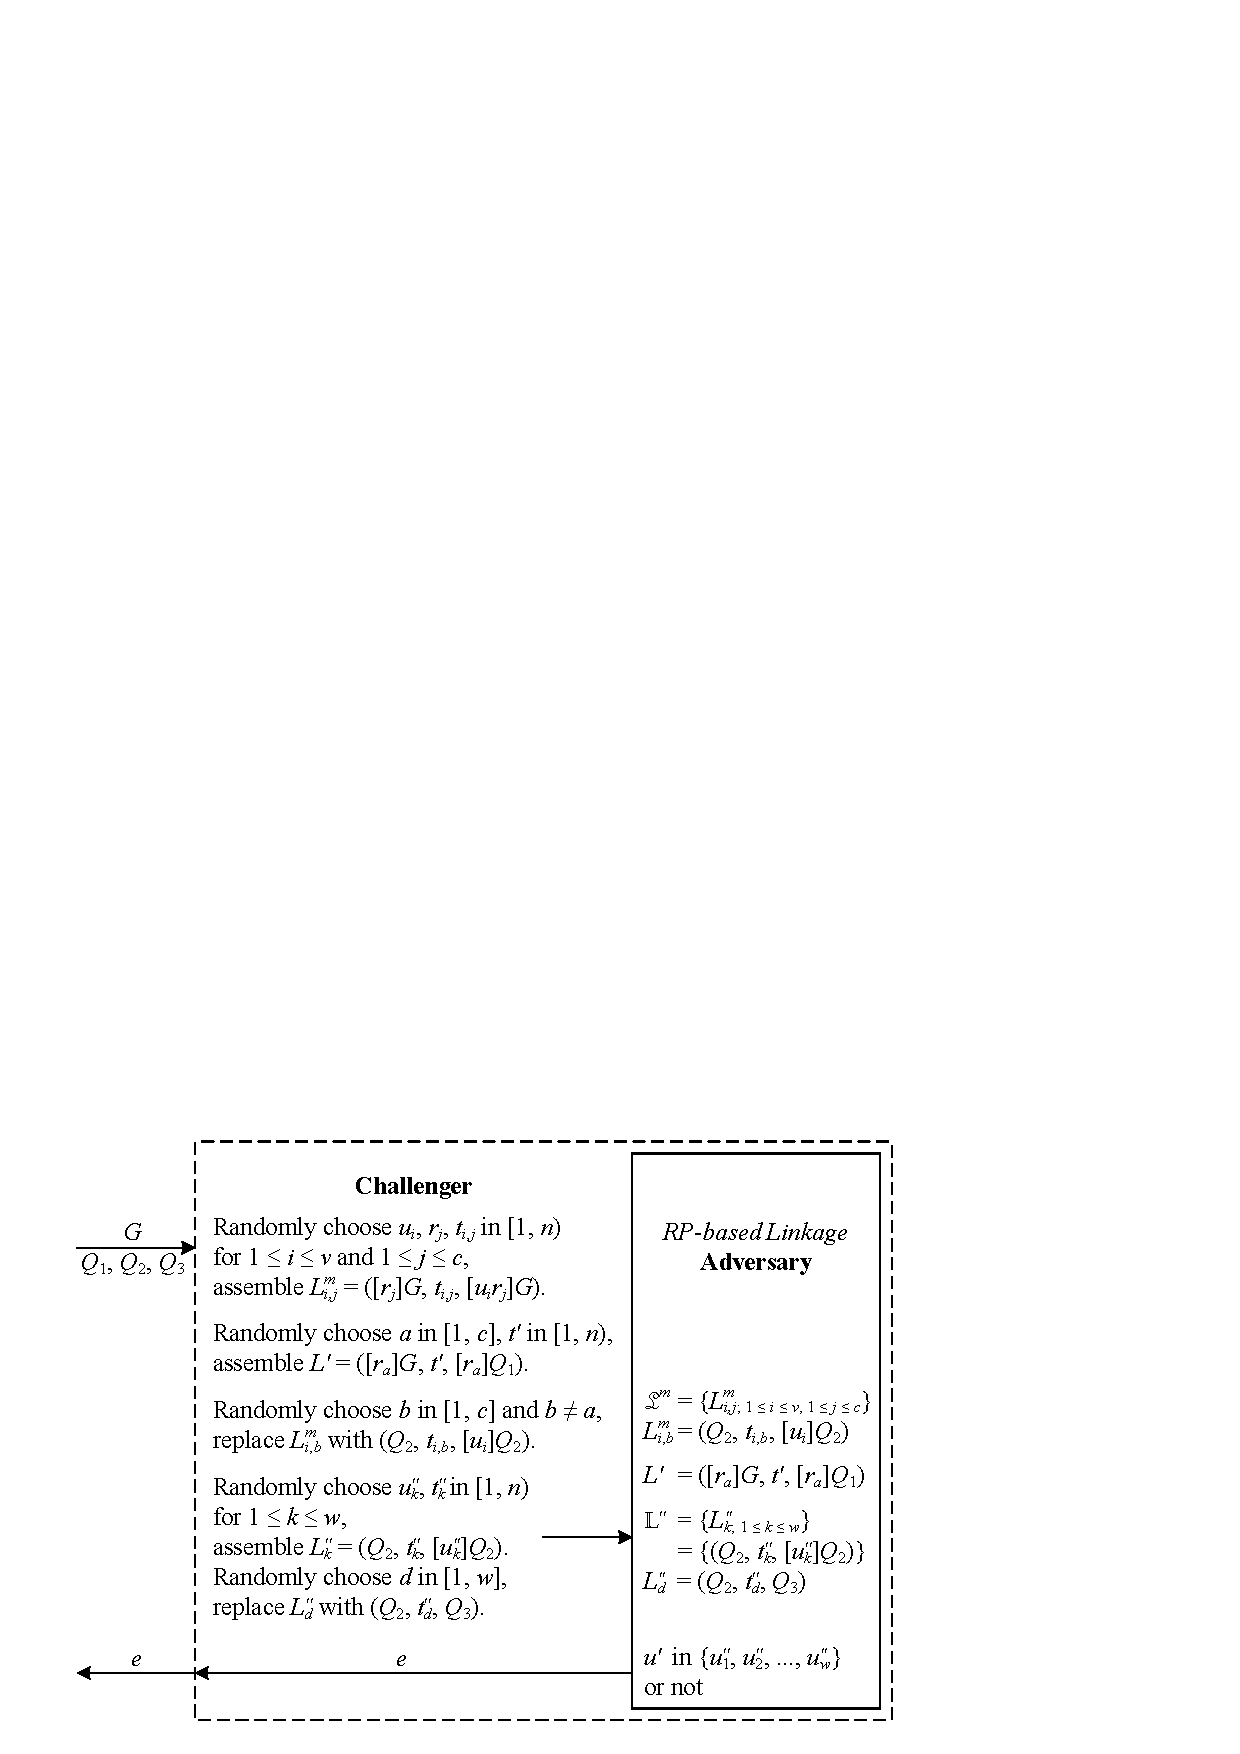
\includegraphics[width=1.0\linewidth]{fig/rp-linkage-game.pdf}
    \caption{The PPT algorithm $\mathcal{D}^*_r$ constructed based on the RP-based linkage game to solve the ECDDH problem.}
    \label{fig:dalgorithm}
  \end{figure}


  The algorithm $\mathcal{D}^*_r$ works as below. (1) Upon receiving an input $(G, Q_1=[x]G, Q_2=[y]G, Q_3=[z]G)$, %of $\mathcal{D}^*_r$
  the challenger
  chooses random numbers in $\mathbb{Z}_n$ to construct $\{u_i\}$, $\{r_j\}$, and $\{t_{i, j}\}$ for $1 \le i \le v$ and $1 \le j \le c$, with which it assembles $L^m_{i, j}=([r_j]G, t_{i,j}, [u_ir_j]G)$.
  In this process, it ensures $[r_{j}]G \neq Q_2$ so that $r_j \neq y$.  % 这个应该反过来讲;因为y是离散对数。
  (2) It randomly chooses $a \in [1, c]$ and $t' \in \mathbb{Z}_n$, to assemble $L' = ([r_{a}]G, t', [r_{a}]Q_1) = ([r_{a}]G, t', [xr_{a}]G)$.
  (3)
  % Here, $L'$ represents the knowledge of the login visiting $RP_{j'}$ by a user with $ID_U = x$.
  Next, the challenger randomly chooses $b \in [1, c]$ and $b \neq a$, and replaces $ID_{RP_b}$ with $Q_2 = [y]G$.
  Hence, for $1 \le i \le v$, the challenger replaces $L^m_{i, b}=([r_b]G, t_{i,b}, [u_ir_b]G)$ with $(Q_2, t_{i,b}, [u_i]Q_2) = ([y]G, t_{i,b}, [u_iy]G)$, and then constructs $\mathfrak{L}^m$.
  (4) the challenger chooses random numbers in $\mathbb{Z}_n$ to construct $\{u''_k\}$ and $\{t''_k\}$ for $1 \leq k \leq w$,
  with which it assembles $\mathbb{L}'' = \{L''_{k; 1\leq k \leq w}\} = \{(Q_2, t''_k, [u''_k]Q_2)\} = \{([y]G, t''_k, [u''_ky]G)\}$.
  In this process, it ensures that $[u''_k]G \neq Q_1$ (i.e., $u''_k \neq x$) and $u''_k \neq u_i$,
  for $1 \le i \le v$ and $1 \le k \le w$.
  Finally, it randomly chooses $d \in [1, w]$ and replaces $L''_{d}$ with $(Q_2, t''_d, Q_3) = ([y]G, t''_d, [z]G)$.
  Thus, $\mathbb{L}'' = \{L''_{k;1\leq k \leq w}\}$ represents the logins initiated by $w$ honest users, i.e., $\mathbf{u}_w=\{u''_1, u''_2, \cdots, u''_{d-1}, z/y, u''_{d+1}, \cdots, u''_w\}$.
  (5) When the adversary of $\mathcal{G}_r$ receives $\mathfrak{L}^m$, $L'$, and $\mathbb{L}''$ from the challenger, it returns $s$ as the output of $\mathcal{D}^*_r$.

  According to the above construction, % of $\mathfrak{L}$, $L'$ and $\mathbb{L}''$,
  $x$ is embedded as $ID_{U'}$ in the login $L'$ visiting the RP with $ID_{RP_{a}} = [r_{a}]G$,
  and $z/y$ is embedded as $ID_{U''_d}$ in $\mathbb{L}''$ visiting the RP with $ID_{RP_{b}}=[y]G$,
  together with $\{u''_1, \cdots, u''_{d-1}, u''_{d+1}, \cdots, u''_w\}$.
  Meanwhile, $[r_{a}]G$ and $[y]G$ are two malicious RPs' identities in $\mathfrak{L}^m$.
  Because $x \neq u''_{k; 1\leq k \leq w, k \neq d}$ and then $x$ is not in $\{u''_1, \cdots, u''_{d-1}, u''_{d+1}, \cdots, u''_w\}$, the adversary outputs $s=1$ and succeeds in the game \emph{only if} $x = z/y$.
  % 这里不是if and only if. "if, 就变成了the adversary必胜了;并不是,而是“有显著的概率”"
  % 当“the adversary outputs s=1 且 succeeds in the game”,=> "x = z/y"
  % 但是,"x = z/y"  => 不能推导得到“the adversary outputs s=1 且 succeeds in the game”。因为adversary有时候fail、不总是succeed
  Therefore, using $\mathcal{D}^*_r$ to solve the ECDDH problem, we have an advantage $\mathbf{Adv}^*=|{\rm Pr}^*_1 - {\rm Pr}^*_2|$, where
  \begin{align*}
  &{\rm Pr}^*_1 =  {\rm Pr}(\mathcal{D}^*_r(G, [x]G, [y]G, [xy]G)=1) \\
  =&{\rm Pr}(\mathcal{G}_r(\mathfrak{L}^m, L', \mathbb{L}'')=1 \; | \; u' \in \mathbf{u}_w) = {\rm Pr}_1 \\
  &{\rm Pr}^*_2= {\rm Pr}(\mathcal{D}^*_r(G, [x]G, [y]G, [z]G)=1) \\
  =&{\rm Pr}(\mathcal{G}_r(\mathfrak{L}^m, L', \mathbb{L}'')=1 \; | \; u' \in \mathbb{Z}_n) = {\rm Pr}_2 \\
  &\mathbf{Adv}^*=|{\rm Pr}^*_1-{\rm Pr}^*_2|=|{\rm Pr}_1-{\rm Pr}_2|={\mathbf{Adv}}
  \end{align*}

  If in $\mathcal{G}_r$ the adversary has a non-negligible advantage, then $\mathbf{Adv}^*={\mathbf{Adv}}$ is also non-negligible regardless of the security parameter $\lambda$. This violates the ECDDH assumption. Therefore, the adversary has no advantage in $\mathcal{G}_r$ and cannot decide whether $L'$ is initiated by some user with an identity in $\mathbf{u}_w$ or by a user in the universal user set.
  Moreover, because $RP_b$ is any malicious RP, this proof can be easily extended from $RP_b$ to more colluding malicious RPs.
  \end{proof}

  \newc
  With Theorem~\ref{rp-privacy-proof}, %we can have that Lemma~\ref{lemma:statically-equivalent} still holds true for the much more complicated model we state above. 
  %Therefore, we can do the similar analysis to prove that $\mathcal{U\!W\!S}^{priv}$ is still RP-private even if we add more RPs, honest users and malicious users into the system.
  we can have that even if colluding RPs and users share 
  $PID_U$s and other information observed in all the logins, 
  the attackers still cannot link any login from an honest user 
  to any other logins from any other honest users to these RPs. 
  Next we want to prove that our web systems $\mathcal{U\!W\!S}^{priv}$ 
  with colluding RPs and users is indistinguishable. 

  Here, we make our proof by contradiction.
  Assuming that the attacker cannot link any login but can 
  distinguish in our web systems for privacy analysis. 
  Then the attacker tell the difference between 
  $\mathcal{U\!W\!S}^{priv}_1$ and $\mathcal{U\!W\!S}^{priv}_2$.
  However, the only difference is that the same honest user login 
  in the same RP in one system but different users in the other, 
  so the attacker can actually link the login by the result of 
  distinguishing. Therefore, there is a contradication to the 
  assumption, where we assumed that the attacker cannot link 
  any login. This shows $\mathcal{U\!W\!S}^{priv}$ with 
  colluding RPs and users is indistinguishable.
  \oldc

  This proves Theorem~\ref{theorem:rp-privacy}.\QED
  
\end{document}
  